\documentclass[]{book}
\usepackage{lmodern}
\usepackage{amssymb,amsmath}
\usepackage{ifxetex,ifluatex}
\usepackage{fixltx2e} % provides \textsubscript
\ifnum 0\ifxetex 1\fi\ifluatex 1\fi=0 % if pdftex
  \usepackage[T1]{fontenc}
  \usepackage[utf8]{inputenc}
\else % if luatex or xelatex
  \ifxetex
    \usepackage{mathspec}
  \else
    \usepackage{fontspec}
  \fi
  \defaultfontfeatures{Ligatures=TeX,Scale=MatchLowercase}
\fi
% use upquote if available, for straight quotes in verbatim environments
\IfFileExists{upquote.sty}{\usepackage{upquote}}{}
% use microtype if available
\IfFileExists{microtype.sty}{%
\usepackage{microtype}
\UseMicrotypeSet[protrusion]{basicmath} % disable protrusion for tt fonts
}{}
\usepackage[margin=1in]{geometry}
\usepackage{hyperref}
\hypersetup{unicode=true,
            pdftitle={R pragmático},
            pdfauthor={Julio Trecenti},
            pdfborder={0 0 0},
            breaklinks=true}
\urlstyle{same}  % don't use monospace font for urls
\usepackage{natbib}
\bibliographystyle{apalike}
\usepackage{color}
\usepackage{fancyvrb}
\newcommand{\VerbBar}{|}
\newcommand{\VERB}{\Verb[commandchars=\\\{\}]}
\DefineVerbatimEnvironment{Highlighting}{Verbatim}{commandchars=\\\{\}}
% Add ',fontsize=\small' for more characters per line
\usepackage{framed}
\definecolor{shadecolor}{RGB}{248,248,248}
\newenvironment{Shaded}{\begin{snugshade}}{\end{snugshade}}
\newcommand{\KeywordTok}[1]{\textcolor[rgb]{0.13,0.29,0.53}{\textbf{{#1}}}}
\newcommand{\DataTypeTok}[1]{\textcolor[rgb]{0.13,0.29,0.53}{{#1}}}
\newcommand{\DecValTok}[1]{\textcolor[rgb]{0.00,0.00,0.81}{{#1}}}
\newcommand{\BaseNTok}[1]{\textcolor[rgb]{0.00,0.00,0.81}{{#1}}}
\newcommand{\FloatTok}[1]{\textcolor[rgb]{0.00,0.00,0.81}{{#1}}}
\newcommand{\ConstantTok}[1]{\textcolor[rgb]{0.00,0.00,0.00}{{#1}}}
\newcommand{\CharTok}[1]{\textcolor[rgb]{0.31,0.60,0.02}{{#1}}}
\newcommand{\SpecialCharTok}[1]{\textcolor[rgb]{0.00,0.00,0.00}{{#1}}}
\newcommand{\StringTok}[1]{\textcolor[rgb]{0.31,0.60,0.02}{{#1}}}
\newcommand{\VerbatimStringTok}[1]{\textcolor[rgb]{0.31,0.60,0.02}{{#1}}}
\newcommand{\SpecialStringTok}[1]{\textcolor[rgb]{0.31,0.60,0.02}{{#1}}}
\newcommand{\ImportTok}[1]{{#1}}
\newcommand{\CommentTok}[1]{\textcolor[rgb]{0.56,0.35,0.01}{\textit{{#1}}}}
\newcommand{\DocumentationTok}[1]{\textcolor[rgb]{0.56,0.35,0.01}{\textbf{\textit{{#1}}}}}
\newcommand{\AnnotationTok}[1]{\textcolor[rgb]{0.56,0.35,0.01}{\textbf{\textit{{#1}}}}}
\newcommand{\CommentVarTok}[1]{\textcolor[rgb]{0.56,0.35,0.01}{\textbf{\textit{{#1}}}}}
\newcommand{\OtherTok}[1]{\textcolor[rgb]{0.56,0.35,0.01}{{#1}}}
\newcommand{\FunctionTok}[1]{\textcolor[rgb]{0.00,0.00,0.00}{{#1}}}
\newcommand{\VariableTok}[1]{\textcolor[rgb]{0.00,0.00,0.00}{{#1}}}
\newcommand{\ControlFlowTok}[1]{\textcolor[rgb]{0.13,0.29,0.53}{\textbf{{#1}}}}
\newcommand{\OperatorTok}[1]{\textcolor[rgb]{0.81,0.36,0.00}{\textbf{{#1}}}}
\newcommand{\BuiltInTok}[1]{{#1}}
\newcommand{\ExtensionTok}[1]{{#1}}
\newcommand{\PreprocessorTok}[1]{\textcolor[rgb]{0.56,0.35,0.01}{\textit{{#1}}}}
\newcommand{\AttributeTok}[1]{\textcolor[rgb]{0.77,0.63,0.00}{{#1}}}
\newcommand{\RegionMarkerTok}[1]{{#1}}
\newcommand{\InformationTok}[1]{\textcolor[rgb]{0.56,0.35,0.01}{\textbf{\textit{{#1}}}}}
\newcommand{\WarningTok}[1]{\textcolor[rgb]{0.56,0.35,0.01}{\textbf{\textit{{#1}}}}}
\newcommand{\AlertTok}[1]{\textcolor[rgb]{0.94,0.16,0.16}{{#1}}}
\newcommand{\ErrorTok}[1]{\textcolor[rgb]{0.64,0.00,0.00}{\textbf{{#1}}}}
\newcommand{\NormalTok}[1]{{#1}}
\usepackage{longtable,booktabs}
\usepackage{graphicx,grffile}
\makeatletter
\def\maxwidth{\ifdim\Gin@nat@width>\linewidth\linewidth\else\Gin@nat@width\fi}
\def\maxheight{\ifdim\Gin@nat@height>\textheight\textheight\else\Gin@nat@height\fi}
\makeatother
% Scale images if necessary, so that they will not overflow the page
% margins by default, and it is still possible to overwrite the defaults
% using explicit options in \includegraphics[width, height, ...]{}
\setkeys{Gin}{width=\maxwidth,height=\maxheight,keepaspectratio}
\IfFileExists{parskip.sty}{%
\usepackage{parskip}
}{% else
\setlength{\parindent}{0pt}
\setlength{\parskip}{6pt plus 2pt minus 1pt}
}
\setlength{\emergencystretch}{3em}  % prevent overfull lines
\providecommand{\tightlist}{%
  \setlength{\itemsep}{0pt}\setlength{\parskip}{0pt}}
\setcounter{secnumdepth}{5}
% Redefines (sub)paragraphs to behave more like sections
\ifx\paragraph\undefined\else
\let\oldparagraph\paragraph
\renewcommand{\paragraph}[1]{\oldparagraph{#1}\mbox{}}
\fi
\ifx\subparagraph\undefined\else
\let\oldsubparagraph\subparagraph
\renewcommand{\subparagraph}[1]{\oldsubparagraph{#1}\mbox{}}
\fi

%%% Use protect on footnotes to avoid problems with footnotes in titles
\let\rmarkdownfootnote\footnote%
\def\footnote{\protect\rmarkdownfootnote}

%%% Change title format to be more compact
\usepackage{titling}

% Create subtitle command for use in maketitle
\newcommand{\subtitle}[1]{
  \posttitle{
    \begin{center}\large#1\end{center}
    }
}

\setlength{\droptitle}{-2em}
  \title{R pragmático}
  \pretitle{\vspace{\droptitle}\centering\huge}
  \posttitle{\par}
  \author{Julio Trecenti}
  \preauthor{\centering\large\emph}
  \postauthor{\par}
  \predate{\centering\large\emph}
  \postdate{\par}
  \date{2016-10-04}

\usepackage{booktabs}

\begin{document}
\maketitle

{
\setcounter{tocdepth}{1}
\tableofcontents
}
\chapter{Setup}\label{setup}

O minicurso ``R pragmático'' é baseado no \texttt{tidyverse} (universo
``arrumado''), um conjunto de pacotes do R que auxiliam o estatístico /
cientista de dados na execução de diversas tarefas corriqueiras de forma
eficiente e unificada. Pense em eficiência, mas não no sentido de
velocidade de execução de algoritmos, mas sim na velocidade de solução
de problemas.

Atualmente, o melhor lugar para aprender sobre o \texttt{tidyverse} é no
livro \href{http://r4ds.had.co.nz/}{R for data science}. Nesse minicurso
abordamos partes desse livro e adicionamos outros, como práticas de
modelgem preditiva e estudos de caso.

\textbf{Público-alvo}

\begin{itemize}
\tightlist
\item
  Estudantes de graduação em estatística que desejam ganhar tempo nos
  trabalhos da faculdade e entrar no mercado de trabalho com bons
  diferenciais.
\item
  Profissionais do mercado de trabalho que desejam inserir o R mo fluxo
  de atividades do setor/empresa.
\item
  Acadêmicos com interesse em tornar suas análises e códigos mais
  legíveis, reprodutíveis, eficientes e organizados.
\end{itemize}

\textbf{Workflow das aulas:}

\begin{itemize}
\tightlist
\item
  Aulas no laboratório de computação (CEC). Não precisa (mas pode) levar
  notebook.
\item
  Exercícios durante as aulas.
\item
  Leituras complementares e opcionais fora da sala de aula.
\end{itemize}

\textbf{Requisitos básicos:}

\begin{itemize}
\tightlist
\item
  Lógica de programação.
\item
  Veja
  \href{http://curso-r.github.io/slides/aula_00_01_apresentacao.html}{essa
  apresentação (aprox. 10 min)} (slides: 13 ao 43).
\item
  Leia esse
  \href{https://blog.rstudio.org/2016/09/15/tidyverse-1-0-0/}{post de
  blog (aprox. 5 min)}.
\item
  Se quiser ganhar tempo, \href{http://github.com}{crie uma conta no
  Github}.
\end{itemize}

\textbf{Conteúdo:}

\begin{itemize}
\tightlist
\item
  Primeiro dia (04/10): introdução ao \texttt{tidyverse}, o operador
  \texttt{pipe}, trabalhando textos com \texttt{stringr}, trabalhando
  datas com \texttt{lubridate}.
\item
  Segundo dia (05/10): transformação de dados com \texttt{dplyr} e
  \texttt{tidyr}, visualização de dados com \texttt{ggplot2}.
\item
  Terceiro dia (06/10): elaboração de relatórios com \texttt{knitr} e
  \texttt{rmarkdown}, modelagem preditiva (parte 1).
\item
  Quarto dia (07/10) modelagem preditiva (parte 2), case studies e
  feedback. R for Data Science
\end{itemize}

\textbf{Não vamos falar de:}

\begin{itemize}
\tightlist
\item
  Programação eficiente com R. Para isso, veja
  \href{https://bookdown.org/csgillespie/efficientR/}{esse livro}, que
  aborda temas importantíssimos como \emph{profiling}, paralelização,
  \texttt{Rcpp}.
\item
  Estudos envolvendo ``big data''. Para isso estude sobre
  \href{http://spark.rstudio.com/}{sparklyr} e
  \href{https://rstudio.github.io/tensorflow/}{tensorflow} e
  \href{https://gist.github.com/Btibert3/7751989}{mongodb}.
\end{itemize}

\section{Diferenças entre C/C++ e R}\label{diferencas-entre-cc-e-r}

Na análise realizada na Seção \ref{inscritos} notei que boa parte dos
inscritos têm background em C/C++. Em uma comparação simples, o foco do
C é eficiência e transparência, enquanto o do R é análise de dados e
interatividade. Isso faz com que as duas linguagens sejam bem
diferentes!

Na prática, temos que

\begin{itemize}
\tightlist
\item
  C é compilável, R é uma linguagem script.
\item
  R é uma linguagem funcional. Por exemplo, \texttt{(}, \texttt{\&} e
  \texttt{+} são funções do R.
\item
  R é vetorizado. Observe esse sacrilégio
\end{itemize}

\begin{Shaded}
\begin{Highlighting}[]
\NormalTok{a <-}\StringTok{ }\KeywordTok{c}\NormalTok{(}\DecValTok{1}\NormalTok{, }\DecValTok{2}\NormalTok{, }\DecValTok{3}\NormalTok{)}
\NormalTok{b <-}\StringTok{ }\KeywordTok{c}\NormalTok{(}\DecValTok{1}\NormalTok{, }\DecValTok{2}\NormalTok{, }\DecValTok{3}\NormalTok{, }\DecValTok{4}\NormalTok{, }\DecValTok{5}\NormalTok{, }\DecValTok{6}\NormalTok{)}
\NormalTok{a +}\StringTok{ }\NormalTok{b }
\end{Highlighting}
\end{Shaded}

\begin{verbatim}
## [1] 2 4 6 5 7 9
\end{verbatim}

Sim, isso funciona! O que acontece aqui é o fenômeno da
\emph{recliclagem} de vetores do R. Caso não esteja acostumado com essas
idiossincrasias do R, veja
\href{http://curso-r.github.io/posts/aula01.html}{essa aula}.

\begin{itemize}
\tightlist
\item
  Você raramente usará loops (\texttt{for}, \texttt{while}) no R. Eles
  são ineficientes e não combinam com o estilo funcional da linguagem.
  Busque sempre realizar as operações com vetores, pois a maioria delas
  são implementadas em C e, portanto, mais eficientes.
\end{itemize}

\section{Pacotes}\label{pacotes}

Se você não está no CEC, precisará instalar alguns pacotes para
acompanhar o curso. Para instalar todas as dependências, rode

\begin{Shaded}
\begin{Highlighting}[]
\KeywordTok{install.packages}\NormalTok{(}\StringTok{'devtools'}\NormalTok{)}
\NormalTok{devtools::}\KeywordTok{install_github}\NormalTok{(}\StringTok{'curso-r/ragmatic'}\NormalTok{)}
\end{Highlighting}
\end{Shaded}

Para visualizar todos os documentos que compõem esse livro, acesse
\href{https://github.com/curso-r/ragmatic-book}{essa página}.

\chapter{Princípios}\label{principios}

\section{O tidyverse}\label{o-tidyverse}

O \texttt{tidyverse} é um pacote do R, cuja única função é carregar
outros pacotes do R. O conjunto desses pacotes forma o
\texttt{tidyverse}. É considerado um ``universo'' a parte do R pois
todas suas ferramentas possuem formas de uso consistentes e funcionam
muito bem em conjunto.

Os princípios do \texttt{tidyverse} seguem abaixo.

\begin{enumerate}
\def\labelenumi{\arabic{enumi}.}
\item
  \textbf{Eficiência algorítmica vs eficiência de trabalho}. Suposição:
  o tempo que o estatísco gasta pensando em como realizar uma operação é
  mais importante do que o tempo que o computador gasta para realizar um
  cálculo.
\item
  \textbf{Tidy data}. Princípio para arrumação de base de dados que
  resolve 90\% dos problemas reais. O objetivo em \emph{arrumação de
  dados} é extrair e transformar uma base de dados até que ela esteja em
  formato \emph{tidy}. Essa é uma boa prática de análise de dados que
  economiza muito tempo em qualquer trabalho. Uma base de dados é
  considerada ``tidy'' se

  \begin{itemize}
  \tightlist
  \item
    Cada observação é uma linha do bd.
  \item
    Cada variável é uma coluna do bd.
  \item
    Cada dado está numa célula do bd.
  \end{itemize}
\item
  \textbf{Utilização do operador \texttt{\%\textgreater{}\%} (pipe)}.

  \begin{quote}
  ``No matter how complex and polished the individual operations are, it
  is often the quality of the glue that most directly determines the
  power of the system.''\\
  -- Hal Abelson
  \end{quote}
\item
  \textbf{Aparato mnemônico}. Pacotes baseados em teoria e API
  consistentes.
\item
  \textbf{Minimalidade e funções puras}. Funções sem
  \emph{side-effects}. Interagem com o mundo através de inputs e
  outputs. Encaixa perfeitamente com o princípio do pipe
\item
  \emph{workflow} para ciência de dados
\end{enumerate}

\section{RStudio}\label{rstudio}

O RStudio é a melhor IDE para usar o R. O programa possui diversas
vantagens e praticamente nenhuma desvantagem. Caso tenha interesse em se
ambientar e entender as características do RStudio, veja
\href{https://csgillespie.github.io/efficientR/set-up.html\#rstudio}{essa
página}.

Uma importante funcionalidade do RStudio é a possibilidade de criar
projetos. Uma estrutura recomendada para organização de pacotes segue
abaixo.

\begin{Shaded}
\begin{Highlighting}[]
\KeywordTok{project/}
  \KeywordTok{-} \NormalTok{README.Rmd   }\CommentTok{# Descrição do pacote}
  \KeywordTok{-} \NormalTok{set-up.R     }\CommentTok{# Pacotes etc}
  \KeywordTok{-} \NormalTok{R/           }\CommentTok{# Código R, organizado com 0-load.R, 1-tidy.R, 2-vis.R, ...}
  \KeywordTok{-} \NormalTok{data/        }\CommentTok{# Dados (estruturados ou não)}
  \KeywordTok{-} \NormalTok{figures/     }\CommentTok{# gráficos (pode ficar dentro de output/)}
  \KeywordTok{-} \NormalTok{output/      }\CommentTok{# Relatórios em .Rmd, .tex etc}
  \KeywordTok{-} \NormalTok{project.Rproj}
\end{Highlighting}
\end{Shaded}

Outra possível forma de estruturar um projeto é organizando-o como um
pacote do R:

\begin{Shaded}
\begin{Highlighting}[]
\KeywordTok{project/}
  \KeywordTok{-} \NormalTok{README.md    }\CommentTok{# Descrição do pacote}
  \KeywordTok{-} \NormalTok{DESCRIPTION  }\CommentTok{# Metadados estruturados do pacote e dependências}
  \KeywordTok{-} \NormalTok{NAMESPACE    }\CommentTok{# importações e exportações do pacote}
  \KeywordTok{-} \NormalTok{vignettes/   }\CommentTok{# Relatórios em .Rmd}
  \KeywordTok{-} \NormalTok{R/           }\CommentTok{# Funções do R}
  \KeywordTok{-} \NormalTok{data/        }\CommentTok{# Dados estruturados (tidy data)}
  \KeywordTok{-} \NormalTok{data-raw/    }\CommentTok{# Dados não estruturados e arqs 0-load.R, 1-tidy.R, 2-vis.R, ...}
  \KeywordTok{-} \NormalTok{project.Rproj}
\end{Highlighting}
\end{Shaded}

Para detalhes de como criar pacotes no R de forma eficiente, leia o
\href{http://r-pkgs.had.co.nz}{r-pkgs}. Recomendo a adoção de um
critério consistente para organização de projetos. O estatístico não
pode perder tempo com a estruturação das pastas, então é melhor forçar
uma estrutura pré-fixada do que planejar a melhor forma de organização
para cada projeto.

\section{RMarkdown}\label{rmarkdown}

O RMarkdown é um tipo de documento especial que contém tanto textos (em
markdown) quanto códigos em R (em chunks). O markdown nada mais é do que
um documento de texto com alguns padrões básicos de formatação, como
negrito, itálico, títulos, subtítulos, itemização e referências
cruzadas. Já os chunks são pedaços de códigos em R encapsulados por três
crases `````''. Os códigos são executados sempre que o documento é
processado para algum formato específico.

A utilização do RMarkdown para produção de relatórios é essencial para o
estatístico pragmático. O RMarkdown possui diversas vantagens:

\begin{enumerate}
\def\labelenumi{\arabic{enumi}.}
\tightlist
\item
  \textbf{Simplicidade e foco}. Obriga o usuário a focar na análise e
  não na formatação do documento.
\item
  \textbf{Versátil}. Pode ser utilizado para gerar documentos em LaTeX,
  Word, HTML e apresentações em beamer, pptx e HTML (de vários tipos).
  Pode ainda gerar sites, livros, dissertações de mestrado e até mesmo
  dashboards interativos.
\item
  \textbf{Reprodutível}. O RMarkdown nada mais é que um arquivo de
  texto. Além disso, ele tenta te obrigar a fazer o documento mais
  autocontido possível. Assim, um documento .Rmd é fácil de compartilhar
  e de ser utilizado pelo receptor. Lembre-se, o receptor pode ser o
  futuro você! Vale enfatizar que a reprodutibilidade é considerada como
  um dos princípios fundamentais para a ciência. Então só de usar
  RMarkdown, você já está colaborando com a ciência :)
\item
  \textbf{Eficiente}. É possível configurar e criar templates de
  análises para quaisquer tipos de aplicações e clientes.
\end{enumerate}

Para detalhes sobre como utilizar o RMarkdown,
\href{http://r4ds.had.co.nz/r-markdown.html}{leia aqui}
\href{http://rmarkdown.rstudio.com/lesson-1.html}{e aqui}.

\section{GitHub}\label{github}

O GitHub é uma plataforma online para compartilhar códigos. Projetos do
GitHub são baseados no \texttt{git}, uma ferramenta de versionamento de
software.

Utilizar o GitHub é uma boa prática de organizar projetos pois é uma
forma de manter os códigos organizados e atualizados na web, sem o
perigo de perder tudo acidentalmente. Esse site também é essencial para
projetos colaborativos, pois aumenta a produtividade e permite que
pessoas de todo lugar ajudem nos projetos. O \texttt{tidyverse} só é o
que é hoje por conta do \emph{social coding}.

Para detalhes, faça o
\href{https://www.coursera.org/learn/data-scientists-tools}{data science
toolbox}.

\section{Pipe}\label{pipe}

O operador \emph{pipe} foi uma das grandes revoluções recentes do R,
tornando a leitura de códigos mais lógica, fácil e compreensível. Este
operador foi introduzido por Stefan Milton Bache no pacote
\texttt{magrittr} e já existem diversos pacotes construidos para
facilitar a sua utilização.

Basicamente, o operador \texttt{\%\textgreater{}\%} usa o resultado do
seu lado esquerdo como primeiro argumento da função do lado direito. Só
isso!

Para usar o operador \texttt{\%\textgreater{}\%}, primeiramente instale
o pacote \texttt{magrittr}.

\begin{Shaded}
\begin{Highlighting}[]
\KeywordTok{install.packages}\NormalTok{(}\StringTok{"magrittr"}\NormalTok{)}
\end{Highlighting}
\end{Shaded}

e carregá-lo com a função \texttt{library()}

\begin{Shaded}
\begin{Highlighting}[]
\KeywordTok{library}\NormalTok{(magrittr)}
\end{Highlighting}
\end{Shaded}

Feito isso, vamos testar o operador calculando a raiz quadrada da soma
de alguns números.

\begin{Shaded}
\begin{Highlighting}[]
\NormalTok{x <-}\StringTok{ }\KeywordTok{c}\NormalTok{(}\DecValTok{1}\NormalTok{, }\DecValTok{2}\NormalTok{, }\DecValTok{3}\NormalTok{, }\DecValTok{4}\NormalTok{)}
\NormalTok{x %>%}\StringTok{ }\NormalTok{sum %>%}\StringTok{ }\NormalTok{sqrt}
\end{Highlighting}
\end{Shaded}

\begin{verbatim}
## [1] 3.162278
\end{verbatim}

O caminho que o código acima seguiu foi enviar o objeto \texttt{x} como
argumento da função \texttt{sum()} e, em seguida, enviar a saida da
expressão \texttt{sum(x)} como argumento da função \texttt{sqrt()}.
Observe que não é necessário colocar os parênteses após o nome das
funções.

Se escrevermos esse cálculo na forma usual, temos o seguinte código:

\begin{Shaded}
\begin{Highlighting}[]
\KeywordTok{sqrt}\NormalTok{(}\KeywordTok{sum}\NormalTok{(x))}
\end{Highlighting}
\end{Shaded}

\begin{verbatim}
## [1] 3.162278
\end{verbatim}

A princípio, a utilização do \texttt{\%\textgreater{}\%} não parece
trazer grandes vantagens, pois a expressão \texttt{sqrt(sum(x))} é
facilmente compreendida. No entanto, se tivermos um grande número de
funções aninhadas, a utilização do \texttt{pipe} transforma um código
confuso e difícil de ser lido em algo simples e intuitivo. Como exemplo,
imagine que você precise escrever uma receita de um bolo usando o R, e
cada passo da receita é uma função:

\begin{Shaded}
\begin{Highlighting}[]
\KeywordTok{esfrie}\NormalTok{(}\KeywordTok{asse}\NormalTok{(}\KeywordTok{coloque}\NormalTok{(}\KeywordTok{bata}\NormalTok{(}\KeywordTok{acrescente}\NormalTok{(}\KeywordTok{recipiente}\NormalTok{(}\KeywordTok{rep}\NormalTok{(}\StringTok{"farinha"}\NormalTok{, }\DecValTok{2}\NormalTok{), }\StringTok{"água"}\NormalTok{, }\StringTok{"fermento"}\NormalTok{, }\StringTok{"leite"}\NormalTok{, }\StringTok{"óleo"}\NormalTok{), }\StringTok{"farinha"}\NormalTok{, até =}\StringTok{ "macio"}\NormalTok{), duraçã}\DataTypeTok{o =} \StringTok{"3min"}\NormalTok{), }\DataTypeTok{lugar =} \StringTok{"forma"}\NormalTok{, }\DataTypeTok{tipo =} \StringTok{"grande"}\NormalTok{, }\DataTypeTok{untada =} \NormalTok{T), duraçã}\DataTypeTok{o =} \StringTok{"50min"}\NormalTok{), }\StringTok{"geladeira"}\NormalTok{, }\StringTok{"20min"}\NormalTok{)}
\end{Highlighting}
\end{Shaded}

Tente entender o que é preciso fazer. Nada fácil, correto? Agora
escrevemos usando o operador \texttt{\%\textgreater{}\%}:

\begin{Shaded}
\begin{Highlighting}[]
\KeywordTok{recipiente}\NormalTok{(}\KeywordTok{rep}\NormalTok{(}\StringTok{"farinha"}\NormalTok{, }\DecValTok{2}\NormalTok{), }\StringTok{"água"}\NormalTok{, }\StringTok{"fermento"}\NormalTok{, }\StringTok{"leite"}\NormalTok{, }\StringTok{"óleo"}\NormalTok{) %>%}
\StringTok{  }\KeywordTok{acrescente}\NormalTok{(}\StringTok{"farinha"}\NormalTok{, até =}\StringTok{ "macio"}\NormalTok{) %>%}
\StringTok{  }\KeywordTok{bata}\NormalTok{(duraçã}\DataTypeTok{o =} \StringTok{"3min"}\NormalTok{) %>%}
\StringTok{  }\KeywordTok{coloque}\NormalTok{(}\DataTypeTok{lugar =} \StringTok{"forma"}\NormalTok{, }\DataTypeTok{tipo =} \StringTok{"grande"}\NormalTok{, }\DataTypeTok{untada =} \NormalTok{T) %>%}
\StringTok{  }\KeywordTok{asse}\NormalTok{(duraçã}\DataTypeTok{o =} \StringTok{"50min"}\NormalTok{) %>%}
\StringTok{  }\KeywordTok{esfrie}\NormalTok{(}\StringTok{"geladeira"}\NormalTok{, }\StringTok{"20min"}\NormalTok{)}
\end{Highlighting}
\end{Shaded}

Agora o código realmente parece uma receita de bolo.

Para mais informações sobre o \texttt{pipe} e exemplos de utilização,
visite a página
\href{http://cran.r-project.org/web/packages/magrittr/vignettes/magrittr.html}{Ceci
n'est pas un pipe}.

\chapter{Análise exploratória: inscritos no curso}\label{set-up}

\begin{Shaded}
\begin{Highlighting}[]
\KeywordTok{library}\NormalTok{(magrittr)}
\KeywordTok{library}\NormalTok{(tidyverse)}
\KeywordTok{library}\NormalTok{(stringr)}
\KeywordTok{library}\NormalTok{(lubridate)}
\KeywordTok{library}\NormalTok{(forcats)}
\end{Highlighting}
\end{Shaded}

\section{Objetivos}\label{objetivos}

\begin{itemize}
\tightlist
\item
  Verificar a bagagem dos alunos.
\item
  Verificar se há concentração de inscritos da graduação.
\item
  Verificar se há diferenças entre a turma do CEC e do Jacy.
\end{itemize}

\section{Base de dados}\label{base-de-dados}

\begin{Shaded}
\begin{Highlighting}[]
\NormalTok{d_alunos <-}\StringTok{ }\KeywordTok{read_csv}\NormalTok{(}\StringTok{'data/lista_anon.csv'}\NormalTok{)}
\KeywordTok{glimpse}\NormalTok{(d_alunos)}
\end{Highlighting}
\end{Shaded}

\begin{verbatim}
## Observations: 95
## Variables: 7
## $ Timestamp                                                                             <chr> ...
## $ Universidade:                                                                         <chr> ...
## $ Estou no(a):                                                                          <chr> ...
## $ Curso:                                                                                <chr> ...
## $ 1. Em que opção você situaria seu conhecimento em R?                                  <chr> ...
## $ 2. Você considera ter conhecimento intermediário/avançado em quais linguagens abaixo? <chr> ...
## $ 3. Você atua no mercado de trabalho?                                                  <chr> ...
\end{verbatim}

\section{Data tidying}\label{data-tidying}

\begin{Shaded}
\begin{Highlighting}[]
\NormalTok{d_alunos %<>%}\StringTok{ }
\StringTok{  }\KeywordTok{mutate}\NormalTok{(}\DataTypeTok{Timestamp =} \KeywordTok{mdy_hms}\NormalTok{(Timestamp)) %>%}\StringTok{ }
\StringTok{  }\KeywordTok{rownames_to_column}\NormalTok{(}\StringTok{'id_pessoa'}\NormalTok{) %>%}\StringTok{ }
\StringTok{  }\KeywordTok{mutate}\NormalTok{(}\DataTypeTok{cec =} \NormalTok{id_pessoa %in%}\StringTok{ }\KeywordTok{as.character}\NormalTok{(}\DecValTok{1}\NormalTok{:}\DecValTok{45}\NormalTok{)) %>%}\StringTok{ }
\StringTok{  }\KeywordTok{gather}\NormalTok{(pergunta, resposta, }\KeywordTok{matches}\NormalTok{(}\StringTok{'^[0-9]'}\NormalTok{)) %>%}\StringTok{ }
\StringTok{  }\KeywordTok{renomear}\NormalTok{() %>%}\StringTok{ }
\StringTok{  }\KeywordTok{spread}\NormalTok{(pergunta, resposta) %>%}\StringTok{ }
\StringTok{  }\KeywordTok{mutate}\NormalTok{(}\DataTypeTok{uni =} \KeywordTok{with}\NormalTok{(., }\KeywordTok{case_when}\NormalTok{(}
    \KeywordTok{str_detect}\NormalTok{(universidade, re_usp) ~}\StringTok{ 'USP'}\NormalTok{,}
    \KeywordTok{str_detect}\NormalTok{(universidade, re_ufscar) ~}\StringTok{ 'UFSCar'}\NormalTok{,}
    \KeywordTok{str_detect}\NormalTok{(universidade, re_unip) ~}\StringTok{ 'UNIP'}\NormalTok{,}
    \OtherTok{TRUE} \NormalTok{~}\StringTok{ 'Outra'}
  \NormalTok{))) %>%}\StringTok{ }
\StringTok{  }\KeywordTok{mutate}\NormalTok{(}\DataTypeTok{esc =} \KeywordTok{with}\NormalTok{(., }\KeywordTok{case_when}\NormalTok{(}
    \KeywordTok{str_detect}\NormalTok{(estou_no_a, }\StringTok{'raduado|formado|Mestrado|Pós'}\NormalTok{) ~}\StringTok{ 'Formado / Pós'}\NormalTok{,}
    \KeywordTok{str_detect}\NormalTok{(estou_no_a, }\StringTok{'Graduação'}\NormalTok{) ~}\StringTok{ 'Graduação'}\NormalTok{,}
    \OtherTok{TRUE} \NormalTok{~}\StringTok{ 'Outra'}
  \NormalTok{))) %>%}\StringTok{ }
\StringTok{  }\KeywordTok{mutate}\NormalTok{(}\DataTypeTok{ime =} \KeywordTok{str_detect}\NormalTok{(universidade, re_ime),}
         \DataTypeTok{cec =} \KeywordTok{if_else}\NormalTok{(cec, }\StringTok{'CEC'}\NormalTok{, }\StringTok{'Jacy'}\NormalTok{))}
\end{Highlighting}
\end{Shaded}

\section{Alguns gráficos}\label{alguns-graficos}

Volume de inscrições no tempo

\begin{Shaded}
\begin{Highlighting}[]
\NormalTok{d_alunos %>%}\StringTok{ }
\StringTok{  }\KeywordTok{arrange}\NormalTok{(timestamp) %>%}\StringTok{ }
\StringTok{  }\KeywordTok{mutate}\NormalTok{(}\DataTypeTok{um =} \DecValTok{1}\NormalTok{, }\DataTypeTok{inscricoes =} \KeywordTok{cumsum}\NormalTok{(um)) %>%}\StringTok{ }
\StringTok{  }\KeywordTok{ggplot}\NormalTok{(}\KeywordTok{aes}\NormalTok{(}\DataTypeTok{x =} \NormalTok{timestamp, }\DataTypeTok{y =} \NormalTok{inscricoes, }\DataTypeTok{colour =} \NormalTok{cec)) +}
\StringTok{  }\KeywordTok{geom_step}\NormalTok{() +}
\StringTok{  }\KeywordTok{geom_hline}\NormalTok{(}\DataTypeTok{yintercept =} \DecValTok{45}\NormalTok{, }\DataTypeTok{colour =} \StringTok{'red'}\NormalTok{, }\DataTypeTok{linetype =} \DecValTok{2}\NormalTok{) +}
\StringTok{  }\KeywordTok{scale_x_datetime}\NormalTok{(}\DataTypeTok{breaks =} \NormalTok{scales::}\KeywordTok{date_breaks}\NormalTok{(}\StringTok{'1 day'}\NormalTok{), }
                   \DataTypeTok{labels =} \NormalTok{scales::}\KeywordTok{date_format}\NormalTok{(}\StringTok{'%b %d'}\NormalTok{)) +}
\StringTok{  }\KeywordTok{scale_y_continuous}\NormalTok{(}\DataTypeTok{breaks =} \DecValTok{0}\NormalTok{:}\DecValTok{4} \NormalTok{*}\StringTok{ }\DecValTok{25}\NormalTok{, }\DataTypeTok{limits =} \KeywordTok{c}\NormalTok{(}\DecValTok{0}\NormalTok{, }\DecValTok{100}\NormalTok{)) +}
\StringTok{  }\KeywordTok{theme_bw}\NormalTok{(}\DecValTok{14}\NormalTok{) +}
\StringTok{  }\KeywordTok{xlab}\NormalTok{(}\StringTok{'Data'}\NormalTok{) +}
\StringTok{  }\KeywordTok{ylab}\NormalTok{(}\StringTok{'Volume de inscrições'}\NormalTok{)}
\end{Highlighting}
\end{Shaded}

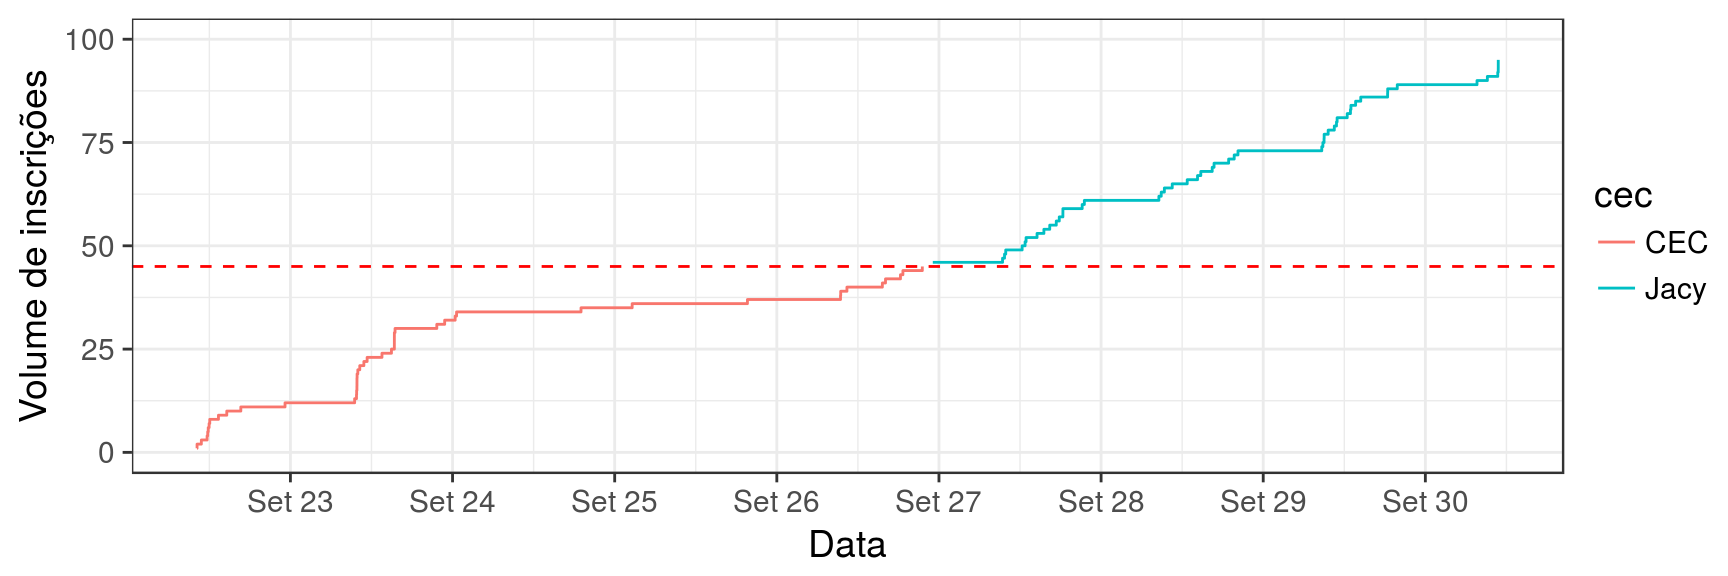
\includegraphics{ragmatic_files/figure-latex/unnamed-chunk-15-1.pdf}

Escolaridade dos inscritos

\begin{Shaded}
\begin{Highlighting}[]
\NormalTok{d_alunos %>%}\StringTok{ }
\StringTok{  }\KeywordTok{replace_na}\NormalTok{(}\KeywordTok{list}\NormalTok{(}\DataTypeTok{esc =} \StringTok{'Outra'}\NormalTok{)) %>%}\StringTok{ }
\StringTok{  }\KeywordTok{mutate}\NormalTok{(}\DataTypeTok{esc =} \KeywordTok{fct_infreq}\NormalTok{(esc)) %>%}\StringTok{ }
\StringTok{  }\KeywordTok{ggplot}\NormalTok{(}\KeywordTok{aes}\NormalTok{(}\DataTypeTok{x =} \NormalTok{esc, }\DataTypeTok{fill =} \NormalTok{cec)) +}
\StringTok{  }\KeywordTok{geom_bar}\NormalTok{(}\DataTypeTok{position =} \StringTok{'dodge'}\NormalTok{) +}
\StringTok{  }\KeywordTok{theme_bw}\NormalTok{(}\DecValTok{14}\NormalTok{) +}
\StringTok{  }\KeywordTok{xlab}\NormalTok{(}\StringTok{''}\NormalTok{) +}
\StringTok{  }\KeywordTok{ylab}\NormalTok{(}\StringTok{'Quantidade de inscritos'}\NormalTok{)}
\end{Highlighting}
\end{Shaded}

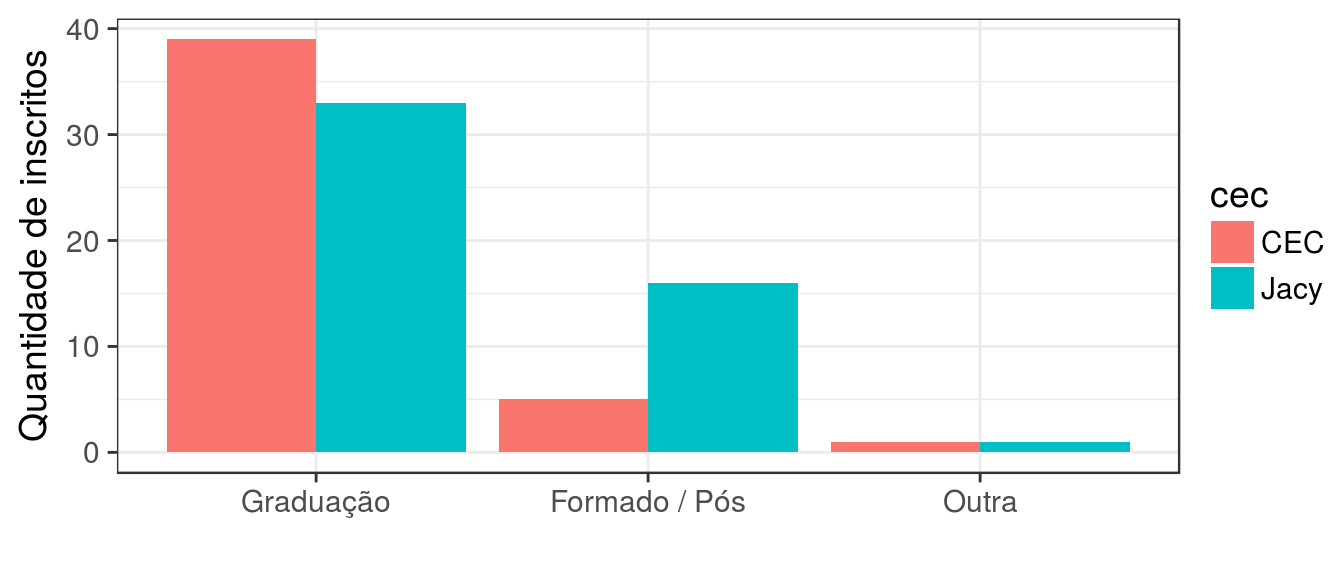
\includegraphics{ragmatic_files/figure-latex/unnamed-chunk-16-1.pdf}

Perguntas 1 e 3: sobre utilização do R.

\begin{Shaded}
\begin{Highlighting}[]
\NormalTok{d_alunos %>%}\StringTok{ }
\StringTok{  }\KeywordTok{gather}\NormalTok{(questao, resposta, }\KeywordTok{matches}\NormalTok{(}\StringTok{'^[13]'}\NormalTok{)) %>%}\StringTok{ }
\StringTok{  }\KeywordTok{replace_na}\NormalTok{(}\KeywordTok{list}\NormalTok{(}\DataTypeTok{resposta =} \StringTok{'Não.'}\NormalTok{)) %>%}\StringTok{ }
\StringTok{  }\KeywordTok{count}\NormalTok{(cec, questao, resposta) %>%}\StringTok{ }
\StringTok{  }\KeywordTok{mutate}\NormalTok{(}\DataTypeTok{prop =} \NormalTok{n /}\StringTok{ }\KeywordTok{sum}\NormalTok{(n)) %>%}\StringTok{ }
\StringTok{  }\KeywordTok{ggplot}\NormalTok{(}\KeywordTok{aes}\NormalTok{(}\DataTypeTok{x =} \KeywordTok{str_wrap}\NormalTok{(resposta, }\DecValTok{20}\NormalTok{), }\DataTypeTok{fill =} \NormalTok{cec, }\DataTypeTok{y =} \NormalTok{prop)) +}
\StringTok{  }\KeywordTok{geom_bar}\NormalTok{(}\DataTypeTok{position =} \StringTok{'dodge'}\NormalTok{, }\DataTypeTok{stat =} \StringTok{'identity'}\NormalTok{) +}
\StringTok{  }\KeywordTok{facet_wrap}\NormalTok{(~questao, }\DataTypeTok{scales =} \StringTok{'free_x'}\NormalTok{, }\DataTypeTok{ncol =} \DecValTok{1}\NormalTok{) +}
\StringTok{  }\KeywordTok{scale_y_continuous}\NormalTok{(}\DataTypeTok{labels =} \NormalTok{scales::percent) +}
\StringTok{  }\KeywordTok{geom_text}\NormalTok{(}\KeywordTok{aes}\NormalTok{(}\DataTypeTok{label =} \NormalTok{scales::}\KeywordTok{percent}\NormalTok{(prop), }\DataTypeTok{group =} \NormalTok{cec), }
            \DataTypeTok{position =} \KeywordTok{position_dodge}\NormalTok{(.}\DecValTok{9}\NormalTok{), }\DataTypeTok{vjust =} \NormalTok{-.}\DecValTok{2}\NormalTok{) +}
\StringTok{  }\KeywordTok{theme_bw}\NormalTok{(}\DecValTok{14}\NormalTok{) +}
\StringTok{  }\KeywordTok{theme}\NormalTok{(}\DataTypeTok{strip.background =} \KeywordTok{element_blank}\NormalTok{()) +}
\StringTok{  }\KeywordTok{xlab}\NormalTok{(}\StringTok{''}\NormalTok{) +}
\StringTok{  }\KeywordTok{ylab}\NormalTok{(}\StringTok{'Proporção de inscritos'}\NormalTok{)}
\end{Highlighting}
\end{Shaded}

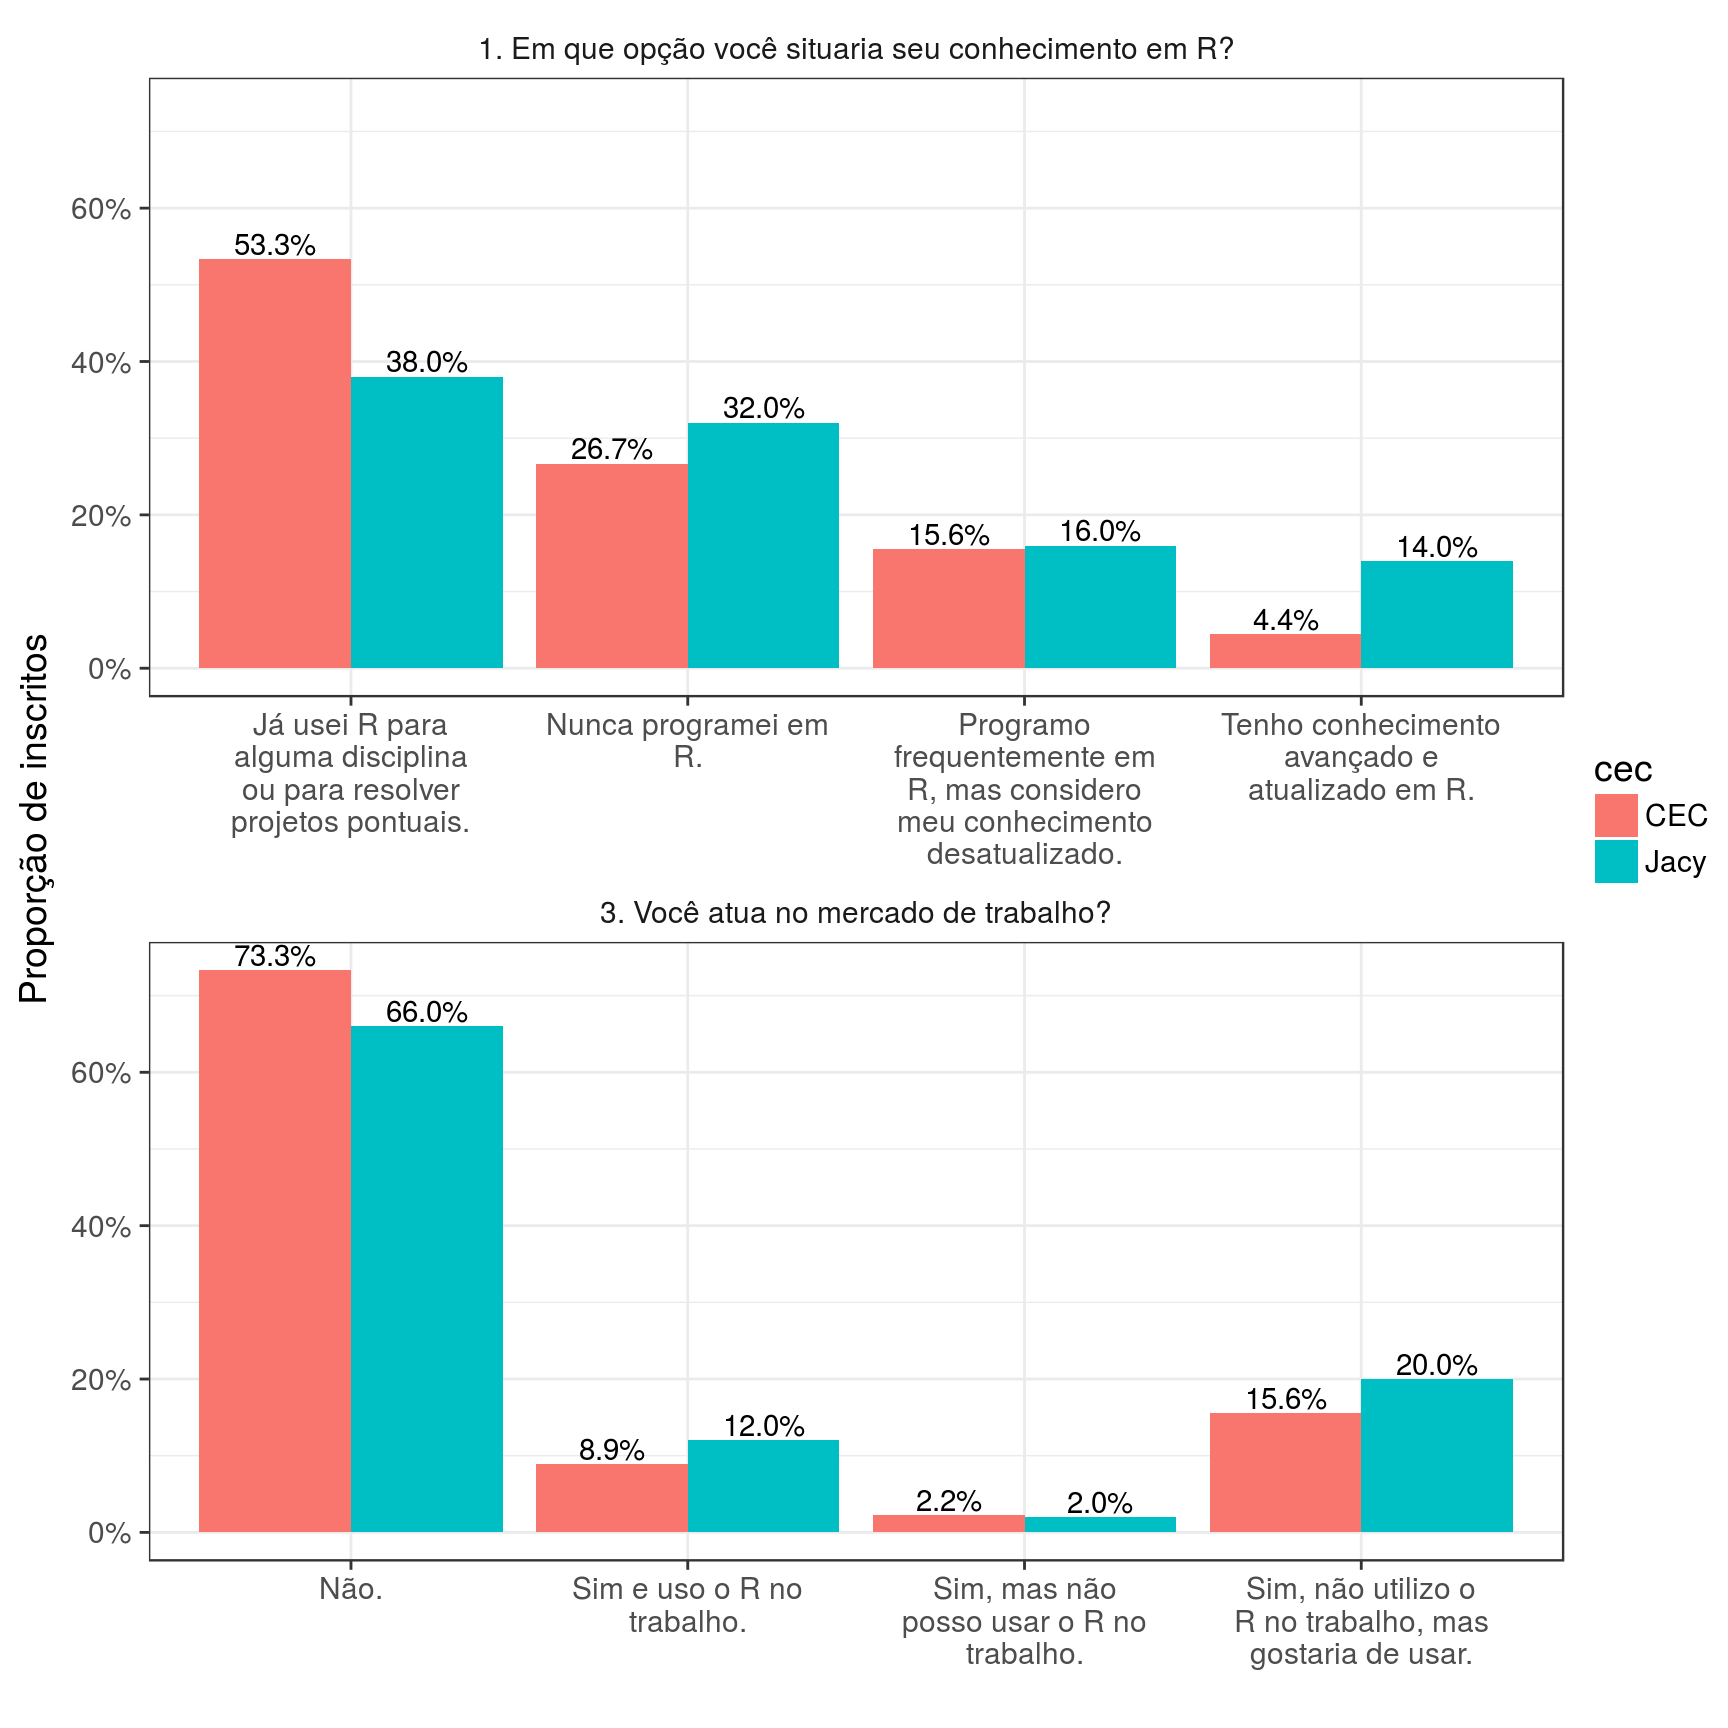
\includegraphics{ragmatic_files/figure-latex/unnamed-chunk-17-1.pdf}

Pergunta 2: sobre conhecimento em outras linguagens. Não soma 100\%!

\begin{Shaded}
\begin{Highlighting}[]
\NormalTok{d_alunos %>%}\StringTok{ }
\StringTok{  }\KeywordTok{gather}\NormalTok{(questao, resposta, }\KeywordTok{matches}\NormalTok{(}\StringTok{'^[2]'}\NormalTok{)) %>%}\StringTok{ }
\StringTok{  }\KeywordTok{replace_na}\NormalTok{(}\KeywordTok{list}\NormalTok{(}\DataTypeTok{resposta =} \StringTok{'Nenhuma'}\NormalTok{)) %>%}\StringTok{ }
\StringTok{  }\KeywordTok{mutate}\NormalTok{(}\DataTypeTok{ling =} \KeywordTok{str_split}\NormalTok{(resposta, }\StringTok{'}\CharTok{\textbackslash{}\textbackslash{}}\StringTok{., '}\NormalTok{)) %>%}\StringTok{ }
\StringTok{  }\KeywordTok{unnest}\NormalTok{(ling) %>%}\StringTok{ }
\StringTok{  }\KeywordTok{mutate}\NormalTok{(}\DataTypeTok{ling =} \KeywordTok{str_replace}\NormalTok{(ling, }\StringTok{'}\CharTok{\textbackslash{}\textbackslash{}}\StringTok{.$'}\NormalTok{, }\StringTok{''}\NormalTok{)) %>%}
\StringTok{  }\KeywordTok{group_by}\NormalTok{(cec) %>%}\StringTok{ }
\StringTok{  }\KeywordTok{mutate}\NormalTok{(}\DataTypeTok{ntot =} \KeywordTok{n_distinct}\NormalTok{(id_pessoa)) %>%}\StringTok{ }
\StringTok{  }\KeywordTok{group_by}\NormalTok{(cec, ling) %>%}\StringTok{ }
\StringTok{  }\KeywordTok{summarise}\NormalTok{(}\DataTypeTok{n =} \KeywordTok{n_distinct}\NormalTok{(id_pessoa), }\DataTypeTok{ntot =} \KeywordTok{first}\NormalTok{(ntot)) %>%}\StringTok{ }
\StringTok{  }\KeywordTok{mutate}\NormalTok{(}\DataTypeTok{prop =} \NormalTok{n /}\StringTok{ }\NormalTok{ntot) %>%}\StringTok{ }
\StringTok{  }\KeywordTok{mutate}\NormalTok{(}\DataTypeTok{ling =} \KeywordTok{str_wrap}\NormalTok{(ling, }\DecValTok{20}\NormalTok{) %>%}\StringTok{ }\KeywordTok{fct_reorder}\NormalTok{(prop, }\DataTypeTok{.desc =} \OtherTok{TRUE}\NormalTok{)) %>%}
\StringTok{  }\KeywordTok{ggplot}\NormalTok{(}\KeywordTok{aes}\NormalTok{(}\DataTypeTok{x =} \NormalTok{ling, }\DataTypeTok{fill =} \NormalTok{cec, }\DataTypeTok{y =} \NormalTok{prop)) +}
\StringTok{  }\KeywordTok{geom_bar}\NormalTok{(}\DataTypeTok{position =} \StringTok{'dodge'}\NormalTok{, }\DataTypeTok{stat =} \StringTok{'identity'}\NormalTok{) +}
\StringTok{  }\KeywordTok{scale_y_continuous}\NormalTok{(}\DataTypeTok{labels =} \NormalTok{scales::percent, }\DataTypeTok{limits =} \KeywordTok{c}\NormalTok{(}\DecValTok{0}\NormalTok{, .}\DecValTok{7}\NormalTok{)) +}
\StringTok{  }\KeywordTok{geom_text}\NormalTok{(}\KeywordTok{aes}\NormalTok{(}\DataTypeTok{label =} \NormalTok{scales::}\KeywordTok{percent}\NormalTok{(prop), }\DataTypeTok{group =} \NormalTok{cec), }
            \DataTypeTok{position =} \KeywordTok{position_dodge}\NormalTok{(.}\DecValTok{9}\NormalTok{), }\DataTypeTok{vjust =} \NormalTok{-.}\DecValTok{2}\NormalTok{) +}
\StringTok{  }\KeywordTok{theme_bw}\NormalTok{(}\DecValTok{14}\NormalTok{) +}
\StringTok{  }\KeywordTok{xlab}\NormalTok{(}\StringTok{'Linguagem de programação'}\NormalTok{) +}
\StringTok{  }\KeywordTok{ylab}\NormalTok{(}\StringTok{'Proporção de inscritos'}\NormalTok{)}
\end{Highlighting}
\end{Shaded}

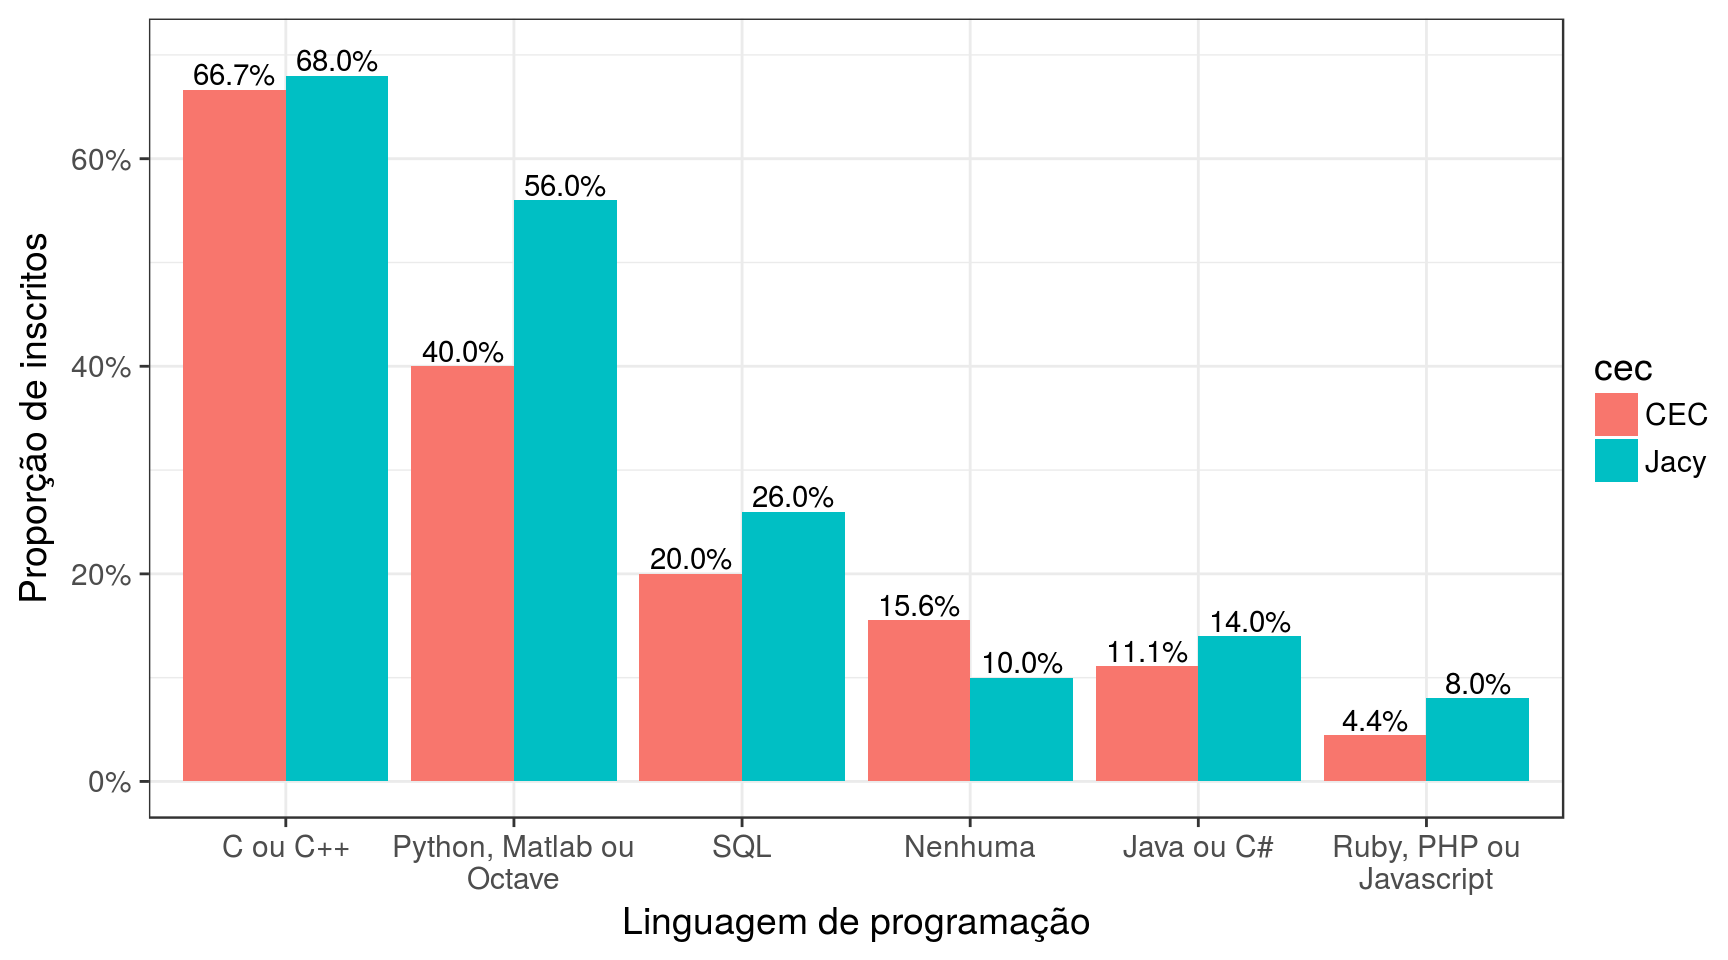
\includegraphics{ragmatic_files/figure-latex/unnamed-chunk-18-1.pdf}

\chapter{Trabalhando com vetores
especiais}\label{trabalhando-com-vetores-especiais}

\section{\texorpdfstring{Pacote \texttt{lubridate} para trabalhar com
datas}{Pacote lubridate para trabalhar com datas}}\label{pacote-lubridate-para-trabalhar-com-datas}

\begin{Shaded}
\begin{Highlighting}[]
\KeywordTok{library}\NormalTok{(magrittr)}
\KeywordTok{library}\NormalTok{(lubridate)}
\end{Highlighting}
\end{Shaded}

Originalmente, o \texttt{R} é bastante ruim para trabalhar com datas, o
que causa frustração e perda de tempo nas análises. O pacote
\texttt{lubridate} foi criado para simplificar ao máximo a leitura de
datas e extração de informações dessas datas.

A função mais importante para leitura de dados no \texttt{lubridate} é a
\texttt{ymd}. Essa função serve para ler qualquer data de uma
\texttt{string} no formato \texttt{YYYY-MM-DD}. Essa função é útil pois
funciona com qualquer separador entre os elementos da data e também
porque temos uma função para cada formato (\texttt{mdy}, \texttt{dmy},
\texttt{dym}, \texttt{myd}, \texttt{ydm}).

\textbf{Exemplo}: dia-ano-mês

\begin{Shaded}
\begin{Highlighting}[]
\NormalTok{d1 <-}\StringTok{ '04/15/06'}
\KeywordTok{dym}\NormalTok{(d1)}
\end{Highlighting}
\end{Shaded}

\begin{verbatim}
## [1] "2015-06-04"
\end{verbatim}

\textbf{Exemplo}: ano-mês-dia

\begin{Shaded}
\begin{Highlighting}[]
\NormalTok{d2 <-}\StringTok{ '2015-01-02'}
\KeywordTok{ymd}\NormalTok{(d2)}
\end{Highlighting}
\end{Shaded}

\begin{verbatim}
## [1] "2015-01-02"
\end{verbatim}

Outras funções importantes

\begin{itemize}
\tightlist
\item
  \texttt{ymd\_hms}: lê datas e horários, generalizando \texttt{ymd}.
  \textbf{Exemplo}:
\end{itemize}

\begin{Shaded}
\begin{Highlighting}[]
\NormalTok{d3 <-}\StringTok{ '07022016 10:11:47'}
\KeywordTok{mdy_hms}\NormalTok{(d3)}
\end{Highlighting}
\end{Shaded}

\begin{verbatim}
## [1] "2016-07-02 10:11:47 UTC"
\end{verbatim}

Observe que as classes são diferentes:

\begin{Shaded}
\begin{Highlighting}[]
\KeywordTok{list}\NormalTok{(}\KeywordTok{ymd}\NormalTok{(d2), }\KeywordTok{mdy_hms}\NormalTok{(d3)) %>%}\StringTok{ }\KeywordTok{lapply}\NormalTok{(class)}
\end{Highlighting}
\end{Shaded}

\begin{verbatim}
## [[1]]
## [1] "Date"
## 
## [[2]]
## [1] "POSIXct" "POSIXt"
\end{verbatim}

\begin{itemize}
\tightlist
\item
  \texttt{year}, \texttt{month}, \texttt{day}, \texttt{quarter},
  \texttt{weekday}, \texttt{week}: extraem componentes da data.
\item
  \texttt{years}, \texttt{months}, \texttt{days}: adicionam tempos a uma
  data, ajudando a criar vetores de datas. Por exemplo
\end{itemize}

\begin{Shaded}
\begin{Highlighting}[]
\KeywordTok{ymd}\NormalTok{(}\StringTok{'2015-01-01'}\NormalTok{) +}\StringTok{ }\KeywordTok{months}\NormalTok{(}\DecValTok{0}\NormalTok{:}\DecValTok{11}\NormalTok{)}
\end{Highlighting}
\end{Shaded}

\begin{verbatim}
##  [1] "2015-01-01" "2015-02-01" "2015-03-01" "2015-04-01" "2015-05-01"
##  [6] "2015-06-01" "2015-07-01" "2015-08-01" "2015-09-01" "2015-10-01"
## [11] "2015-11-01" "2015-12-01"
\end{verbatim}

\begin{itemize}
\tightlist
\item
  \texttt{floor\_date} e \texttt{ceiling\_date}: arredonda datas para
  uma unidade de interesse. Útil para agregar dados diários por semana,
  mês, trimestre etc.
\end{itemize}

Mais informações: ver
\href{https://cran.r-project.org/web/packages/lubridate/vignettes/lubridate.html}{aqui}
e
\href{https://www.jstatsoft.org/index.php/jss/article/view/v040i03/v40i03.pdf}{aqui}.

\subsection{Exercício}\label{exercicio}

(\ldots{})

\section{\texorpdfstring{Pacote \texttt{stringr} para trabalhar com
textos}{Pacote stringr para trabalhar com textos}}\label{pacote-stringr-para-trabalhar-com-textos}

O R básico não tem uma sintaxe consistente para trabalhar com textos. O
pacote \texttt{stringr} ajuda a realizar todas as tarefas básicas de
manipulação de texto, exigindo que o usuário estude apenas uma sintaxe.
O \texttt{stringr} também é construído sobre a
\href{http://site.icu-project.org/}{biblioteca ICU}, implementada em
\texttt{C} e \texttt{C++}, apresentando resultados rápidos e confiáveis.

As regras básicas do pacote são:

\begin{itemize}
\tightlist
\item
  As funções de manipulação de texto começam com \texttt{str\_}. Caso
  esqueça o nome de uma função, basta digitar \texttt{stringr::str\_} e
  apertar \texttt{TAB} para ver quais são as opções.
\item
  O primeiro argumento da função é sempre uma \texttt{string}.
\end{itemize}

Antes de listar as funções, precisamos estudar o básico de expressões
regulares.

\subsection{Expressões regulares}\label{expressoes-regulares}

Expressão regular ou \emph{regex} é uma sequência concisa de caracteres
que representa várias strings. Entender o básico de expressões regulares
é indispensável para trabalhar com textos.

Vamos estudar expressões regulares através de exemplos e com a função
\texttt{str\_detect()}. Essa função retorna \texttt{TRUE} se uma string
atende à uma expressão regular e \texttt{FALSE} em caso contrário.

A tabela abaixo mostra a aplicação de seis \texttt{regex} a seis strings
distintas.

\begin{Shaded}
\begin{Highlighting}[]
\KeywordTok{library}\NormalTok{(stringr)}
\NormalTok{testes <-}\StringTok{ }\KeywordTok{c}\NormalTok{(}\StringTok{'ban'}\NormalTok{, }\StringTok{'banana'}\NormalTok{, }\StringTok{'abandonado'}\NormalTok{, }\StringTok{'pranab anderson'}\NormalTok{, }\StringTok{'BANANA'}\NormalTok{, }\StringTok{'ele levou ban'}\NormalTok{)}

\NormalTok{expressoes <-}\StringTok{ }\KeywordTok{list}\NormalTok{(}
  \StringTok{'ban'}\NormalTok{, }\CommentTok{# reconhece tudo que tenha "ban", mas não ignora case}
  \StringTok{'BAN'}\NormalTok{, }\CommentTok{# reconhece tudo que tenha "BAN", mas não ignora case}
  \KeywordTok{regex}\NormalTok{(}\StringTok{'ban'}\NormalTok{, }\DataTypeTok{ignore_case =} \OtherTok{TRUE}\NormalTok{), }\CommentTok{# reconhece tudo que tenha "ban", ignorando case}
  \StringTok{'ban$'}\NormalTok{, }\CommentTok{# reconhece apenas o que termina exatamente em "ban"}
  \StringTok{'^ban'}\NormalTok{, }\CommentTok{# reconhece apenas o que começa exatamente com "ban"}
  \StringTok{'b ?an'} \CommentTok{# reconhece tudo que tenha "ban", com ou sem espaço entre o "b" e o "a"}
\NormalTok{)}
\end{Highlighting}
\end{Shaded}

\begin{tabular}{l|l|l|l|l|l|l}
\hline
regex & ban & banana & abandonado & pranab anderson & BANANA & ele levou ban\\
\hline
ban & TRUE & TRUE & TRUE & FALSE & FALSE & TRUE\\
\hline
BAN & FALSE & TRUE & FALSE & FALSE & FALSE & FALSE\\
\hline
ban & FALSE & FALSE & TRUE & FALSE & FALSE & FALSE\\
\hline
ban\$ & FALSE & FALSE & FALSE & TRUE & FALSE & FALSE\\
\hline
\textasciicircum{}ban & FALSE & FALSE & FALSE & FALSE & TRUE & FALSE\\
\hline
b ?an & FALSE & FALSE & FALSE & FALSE & FALSE & TRUE\\
\hline
\end{tabular}

\subsubsection{Quantificadores}\label{quantificadores}

Os caracteres \texttt{+}, \texttt{*} e \texttt{\{x,y\}} indicam quantas
vezes um padrão se repete:

\begin{itemize}
\tightlist
\item
  \texttt{ey+} significa \texttt{e} e depois \texttt{y} ``\textbf{uma
  vez} ou mais''. Por exemplo, reconhece \texttt{hey}, \texttt{heyy},
  \texttt{a\ eyyy}, mas não reconhece \texttt{e}, \texttt{y} nem
  \texttt{yy}.
\item
  \texttt{ey*} significa ``\textbf{zero vezes} ou mais''. Por exemplo,
  reconhece \texttt{hey}, \texttt{heyy}, \texttt{a\ eyyy} e \texttt{e},
  mas não reconhece \texttt{y} nem \texttt{yy}.
\item
  \texttt{ey\{3\}} significa ``exatamente três vezes''. Por exemplo,
  reconhece \texttt{eyyy} e \texttt{eyyyy}, mas não reconhece
  \texttt{eyy}.
\item
  \texttt{ey\{1,3\}} significa ``entre uma e três vezes''.
\end{itemize}

Para aplicar um quantificador a um conjunto de caracteres, use
parênteses. Por exemplo, \texttt{(ey\ )+} reconhece \texttt{ey\ ey}.

\subsubsection{Conjuntos}\label{conjuntos}

Colocando caracteres dentro de \texttt{{[}{]}}, reconhecemos quaisquer
caracteres desse conjunto. Alguns exemplos práticos:

\begin{itemize}
\tightlist
\item
  \texttt{{[}Cc{]}asa} para reconhecer ``casa'' em maiúsculo ou
  minúsculo.
\item
  \texttt{{[}0-9{]}} para reconhecer somente números. O mesmo vale para
  letras \texttt{{[}a-z{]}}, \texttt{{[}A-Z{]}}, \texttt{{[}a-zA-Z{]}}
  etc.
\item
  O símbolo \texttt{\^{}} dentro do colchete significa negação. Por
  exemplo, \texttt{{[}\^{}0-9{]}} significa pegar tudo o que não é
  número.
\item
  O símbolo \texttt{.} fora do colchete indica ``qualquer caractere'',
  mas dentro do colchete é apenas ponto.
\item
  Use \texttt{{[}{[}:space:{]}{]}+} para reconhecer espaços e
  \texttt{{[}{[}:punct:{]}{]}+} para reconhecer pontuações.
\end{itemize}

\subsubsection{Miscelânea}\label{miscelanea}

\begin{itemize}
\tightlist
\item
  Use \texttt{abjutils::rm\_accent()} para retirar os acentos de um
  texto.
\item
  Use \texttt{\textbar{}} para opções, por exemplo
  \texttt{desfavor\textbar{}desprov} reconhece tanto ``desfavorável''
  quanto ``desprovido''
\item
  \texttt{\textbackslash{}n} pula linha, \texttt{\textbackslash{}f} é
  final da página, \texttt{\textbackslash{}t} é tab. Use
  \texttt{\textbackslash{}} para transformar caracteres especiais em
  literais.
\item
  \texttt{tolower()} e \texttt{toupper()} para mudar o case de uma
  string.
\end{itemize}

A lista de possibilidades com expressões regulares é extensa. Um bom
lugar para testar o funcionamento de expressões regulares é o
\href{https://regex101.com/}{regex101}.

\subsection{\texorpdfstring{Funções do
\texttt{stringr}}{Funções do stringr}}\label{funcoes-do-stringr}

\begin{itemize}
\item
  \texttt{str\_detect()} retorna \texttt{TRUE} se a regex é compatível
  com a string e \texttt{FALSE} caso contrário
\item
  \texttt{str\_lengh()} retorna o comprimento de uma string.
\end{itemize}

\begin{Shaded}
\begin{Highlighting}[]
\KeywordTok{str_length}\NormalTok{(}\StringTok{'hye'}\NormalTok{)}
\end{Highlighting}
\end{Shaded}

\begin{verbatim}
## [1] 3
\end{verbatim}

\begin{itemize}
\tightlist
\item
  \texttt{str\_trim()} retira espaços e quebras de linha/tabs no início
  ou final de string.
\end{itemize}

\begin{Shaded}
\begin{Highlighting}[]
\NormalTok{string <-}\StringTok{ '}\CharTok{\textbackslash{}n}\StringTok{essa      string é muito suja       }\CharTok{\textbackslash{}n}\StringTok{'}
\KeywordTok{str_trim}\NormalTok{(string)}
\end{Highlighting}
\end{Shaded}

\begin{verbatim}
## [1] "essa      string é muito suja"
\end{verbatim}

\begin{itemize}
\tightlist
\item
  \texttt{str\_replace()} e \texttt{str\_replace\_all()} substituem um
  padrão (ou todos) encontrado para um outro padrão
\end{itemize}

\begin{Shaded}
\begin{Highlighting}[]
\NormalTok{string <-}\StringTok{ 'heyyy ui yy'}
\KeywordTok{str_replace}\NormalTok{(string, }\StringTok{'y'}\NormalTok{, }\StringTok{'x'}\NormalTok{)}
\end{Highlighting}
\end{Shaded}

\begin{verbatim}
## [1] "hexyy ui yy"
\end{verbatim}

\begin{Shaded}
\begin{Highlighting}[]
\KeywordTok{str_replace}\NormalTok{(string, }\StringTok{'y+'}\NormalTok{, }\StringTok{'x'}\NormalTok{)}
\end{Highlighting}
\end{Shaded}

\begin{verbatim}
## [1] "hex ui yy"
\end{verbatim}

\begin{Shaded}
\begin{Highlighting}[]
\KeywordTok{str_replace_all}\NormalTok{(string, }\StringTok{'y'}\NormalTok{, }\StringTok{'x'}\NormalTok{)}
\end{Highlighting}
\end{Shaded}

\begin{verbatim}
## [1] "hexxx ui xx"
\end{verbatim}

\begin{Shaded}
\begin{Highlighting}[]
\KeywordTok{str_replace_all}\NormalTok{(}\StringTok{'string     com    muitos espaços'}\NormalTok{, }\StringTok{' +'}\NormalTok{, }\StringTok{' '}\NormalTok{) }\CommentTok{# tirar espaços extras}
\end{Highlighting}
\end{Shaded}

\begin{verbatim}
## [1] "string com muitos espaços"
\end{verbatim}

\begin{itemize}
\tightlist
\item
  \texttt{str\_match()} e \texttt{str\_match\_all()} extrai pedaços da
  string identificados pela regex. Caso queira extrair somente a parte
  identificada, use parênteses.
\end{itemize}

\begin{Shaded}
\begin{Highlighting}[]
\NormalTok{frases <-}\StringTok{ }\KeywordTok{c}\NormalTok{(}\StringTok{'a roupa do rei'}\NormalTok{, }\StringTok{'de roma'}\NormalTok{, }\StringTok{'o rato roeu'}\NormalTok{)}
\KeywordTok{str_match}\NormalTok{(frases, }\StringTok{'roe'}\NormalTok{)}
\end{Highlighting}
\end{Shaded}

\begin{verbatim}
##      [,1] 
## [1,] NA   
## [2,] NA   
## [3,] "roe"
\end{verbatim}

\begin{Shaded}
\begin{Highlighting}[]
\KeywordTok{str_match_all}\NormalTok{(frases, }\StringTok{'ro'}\NormalTok{)}
\end{Highlighting}
\end{Shaded}

\begin{verbatim}
## [[1]]
##      [,1]
## [1,] "ro"
## 
## [[2]]
##      [,1]
## [1,] "ro"
## 
## [[3]]
##      [,1]
## [1,] "ro"
\end{verbatim}

\begin{Shaded}
\begin{Highlighting}[]
\KeywordTok{str_match}\NormalTok{(frases, }\StringTok{'o (ro)'}\NormalTok{)}
\end{Highlighting}
\end{Shaded}

\begin{verbatim}
##      [,1]   [,2]
## [1,] NA     NA  
## [2,] NA     NA  
## [3,] "o ro" "ro"
\end{verbatim}

\begin{itemize}
\tightlist
\item
  \texttt{str\_split()} separa uma string em várias de acordo com um
  separador.
\end{itemize}

\begin{Shaded}
\begin{Highlighting}[]
\NormalTok{string <-}\StringTok{ 'eu sei, usar virgulas, de forma, perfeita'}

\KeywordTok{str_split}\NormalTok{(string, }\StringTok{', '}\NormalTok{)}
\end{Highlighting}
\end{Shaded}

\begin{verbatim}
## [[1]]
## [1] "eu sei"        "usar virgulas" "de forma"      "perfeita"
\end{verbatim}

\begin{Shaded}
\begin{Highlighting}[]
\KeywordTok{str_split}\NormalTok{(string, }\StringTok{', '}\NormalTok{, }\DataTypeTok{simplify =} \OtherTok{TRUE}\NormalTok{)}
\end{Highlighting}
\end{Shaded}

\begin{verbatim}
##      [,1]     [,2]            [,3]       [,4]      
## [1,] "eu sei" "usar virgulas" "de forma" "perfeita"
\end{verbatim}

\begin{itemize}
\tightlist
\item
  \texttt{str\_split\_fixed()} faz o mesmo que \texttt{str\_split()},
  mas separa apenas \texttt{n} vezes
\end{itemize}

\begin{Shaded}
\begin{Highlighting}[]
\KeywordTok{str_split_fixed}\NormalTok{(string, }\StringTok{', '}\NormalTok{, }\DecValTok{3}\NormalTok{)}
\end{Highlighting}
\end{Shaded}

\begin{verbatim}
##      [,1]     [,2]            [,3]                
## [1,] "eu sei" "usar virgulas" "de forma, perfeita"
\end{verbatim}

\begin{Shaded}
\begin{Highlighting}[]
\KeywordTok{str_split_fixed}\NormalTok{(string, }\StringTok{', '}\NormalTok{, }\DecValTok{4}\NormalTok{) }\CommentTok{# igual a str_split(string, simplify = TRUE)}
\end{Highlighting}
\end{Shaded}

\begin{verbatim}
##      [,1]     [,2]            [,3]       [,4]      
## [1,] "eu sei" "usar virgulas" "de forma" "perfeita"
\end{verbatim}

\begin{itemize}
\tightlist
\item
  \texttt{str\_sub()} extrai uma parte da string de acordo com os
  índices.
\end{itemize}

\begin{Shaded}
\begin{Highlighting}[]
\NormalTok{string <-}\StringTok{ 'quero pegar só uma parte disso'}
\KeywordTok{str_sub}\NormalTok{(string, }\DecValTok{13}\NormalTok{, }\DecValTok{14}\NormalTok{)}
\end{Highlighting}
\end{Shaded}

\begin{verbatim}
## [1] "só"
\end{verbatim}

\begin{Shaded}
\begin{Highlighting}[]
\KeywordTok{str_sub}\NormalTok{(string, -}\DecValTok{5}\NormalTok{, -}\DecValTok{1}\NormalTok{) }\CommentTok{# usar números negativos para voltar do final da string}
\end{Highlighting}
\end{Shaded}

\begin{verbatim}
## [1] "disso"
\end{verbatim}

\begin{Shaded}
\begin{Highlighting}[]
\NormalTok{indices <-}\StringTok{ }\KeywordTok{str_locate}\NormalTok{(string, }\StringTok{'parte'}\NormalTok{)}
\NormalTok{indices}
\end{Highlighting}
\end{Shaded}

\begin{verbatim}
##      start end
## [1,]    20  24
\end{verbatim}

\begin{Shaded}
\begin{Highlighting}[]
\KeywordTok{str_sub}\NormalTok{(string, indices) }\CommentTok{# pode ser útil usar com str_locate.}
\end{Highlighting}
\end{Shaded}

\begin{verbatim}
## [1] "parte"
\end{verbatim}

\begin{itemize}
\tightlist
\item
  \texttt{str\_subset()} retorna somente as strings compatíveis com a
  regex.
\end{itemize}

\begin{Shaded}
\begin{Highlighting}[]
\NormalTok{frases <-}\StringTok{ }\KeywordTok{c}\NormalTok{(}\StringTok{'a roupa do rei'}\NormalTok{, }\StringTok{'de roma'}\NormalTok{, }\StringTok{'o rato roeu'}\NormalTok{)}
\KeywordTok{str_subset}\NormalTok{(frases, }\StringTok{'d[eo]'}\NormalTok{)}
\end{Highlighting}
\end{Shaded}

\begin{verbatim}
## [1] "a roupa do rei" "de roma"
\end{verbatim}

\subsection{Exemplo}\label{exemplo}

\subsection{Exercícios}\label{exercicios}

\begin{enumerate}
\def\labelenumi{\arabic{enumi}.}
\tightlist
\item
  Considere o seguinte texto
\end{enumerate}

\begin{Shaded}
\begin{Highlighting}[]
\NormalTok{txt <-}\StringTok{ "A função mais importante para leitura de dados no `lubridate` é a `ymd`. Essa função serve para ler qualquer data de uma `string` no formato `YYYY-MM-DD`. Essa função é útil pois funciona com qualquer separador entre os elementos da data e também porque temos uma função para cada formato (`mdy`, `dmy`, `dym`, `myd`, `ydm`)."}
\end{Highlighting}
\end{Shaded}

Extraia todas as combinações da função \texttt{ymd}, sem repetições.

\begin{enumerate}
\def\labelenumi{\arabic{enumi}.}
\setcounter{enumi}{1}
\tightlist
\item
  Considere os textos abaixo
\end{enumerate}

\begin{Shaded}
\begin{Highlighting}[]
\NormalTok{txts <-}\StringTok{ }\KeywordTok{c}\NormalTok{(}
  \StringTok{'o produto é muito bom'}\NormalTok{,}
  \StringTok{'o produto não é bom'}\NormalTok{,}
  \StringTok{'o produto não é muito bom'}\NormalTok{,}
  \StringTok{'o produto não é ruim'}\NormalTok{,}
  \StringTok{'o produto não é não bom'}
\NormalTok{)}
\end{Highlighting}
\end{Shaded}

Crie uma regra para identificar se o texto refere-se a um feedback
positivo ou negativo sobre o produto (considera não bom = ruim e
vice-versa). Retorne um vetor lógico que vale \texttt{TRUE} se o
feedback é positivo e \texttt{FALSE} caso contrário.

\section{\texorpdfstring{Pacote \texttt{forcats} para trabalhar com
factors}{Pacote forcats para trabalhar com factors}}\label{pacote-forcats-para-trabalhar-com-factors}

Factors sempre foram uma pedra no sapato para usuários de R. Esses
objetos são estranhos pois parecem textos, mas na verdade são inteiros.

\begin{Shaded}
\begin{Highlighting}[]
\NormalTok{x <-}\StringTok{ }\KeywordTok{factor}\NormalTok{(}\KeywordTok{c}\NormalTok{(}\StringTok{'a'}\NormalTok{, }\StringTok{'b'}\NormalTok{, }\StringTok{'c'}\NormalTok{))}
\NormalTok{x}
\end{Highlighting}
\end{Shaded}

\begin{verbatim}
## [1] a b c
## Levels: a b c
\end{verbatim}

\begin{Shaded}
\begin{Highlighting}[]
\KeywordTok{typeof}\NormalTok{(x)}
\end{Highlighting}
\end{Shaded}

\begin{verbatim}
## [1] "integer"
\end{verbatim}

Assim, eles podem levar a erros do tipo:

\begin{Shaded}
\begin{Highlighting}[]
\NormalTok{x <-}\StringTok{ }\KeywordTok{factor}\NormalTok{(}\KeywordTok{c}\NormalTok{(}\StringTok{'6'}\NormalTok{, }\StringTok{'5'}\NormalTok{, }\StringTok{'4'}\NormalTok{))}
\KeywordTok{as.numeric}\NormalTok{(x)}
\end{Highlighting}
\end{Shaded}

\begin{verbatim}
## [1] 3 2 1
\end{verbatim}

O problema é que, historicamente, esses objetos eram utilizados por
diversos objetos do R. Em particular, o \texttt{data.frame} até hoje
utiliza fatores como padrão. Felizmente, o \texttt{tidyverse} nos livra
desse mal e permite que utilizemos fatores somente quando eles são
realmente úteis.

Mas quando fatores são úteis? A resposta para essa pergunta vem da
própria estatística: temos dois tipos de variáveis categóricas
existentes, a nominal e a ordinal. Uma variável nominal pode ser
completamente representada por um vetor de strings. Mas isso não vale
para variáveis ordinais, pois um vetor de strings só pode ser ordenado
alfabeticamente, o que em muitos casos não é suficiente. O
\texttt{factor} permite que associemos um inteiro para cada valor de uma
string, nos dando a possibilidade de ordená-las da forma que quisermos.

O pacote \texttt{forcats} (\texttt{for} - para, \texttt{cats} -
categóricas, não gatos) serve justamente para reordenar fatores de
diversas formas. Isso é especialmente útil para visualização, pois
muitas vezes queremos ordenar coisas de acordo com alguma regra.

Por exemplo, considere o seguinte gráfico de barras (veremos sobre o
ggplot na próxima vez).

\begin{Shaded}
\begin{Highlighting}[]
\KeywordTok{set.seed}\NormalTok{(}\DecValTok{123}\NormalTok{)}
\NormalTok{labs <-}\StringTok{ }\KeywordTok{c}\NormalTok{(}\StringTok{'banana'}\NormalTok{, }\StringTok{'maçã'}\NormalTok{, }\StringTok{'laranja'}\NormalTok{, }\StringTok{'limão'}\NormalTok{, }\StringTok{'pêssego'}\NormalTok{)[}\KeywordTok{rbinom}\NormalTok{(}\DecValTok{1000}\NormalTok{, }\DecValTok{4}\NormalTok{, .}\DecValTok{2}\NormalTok{) +}\StringTok{ }\DecValTok{1}\NormalTok{]}
\NormalTok{labs %>%}\StringTok{ }\NormalTok{ggplot2::}\KeywordTok{qplot}\NormalTok{()}
\end{Highlighting}
\end{Shaded}

\begin{center}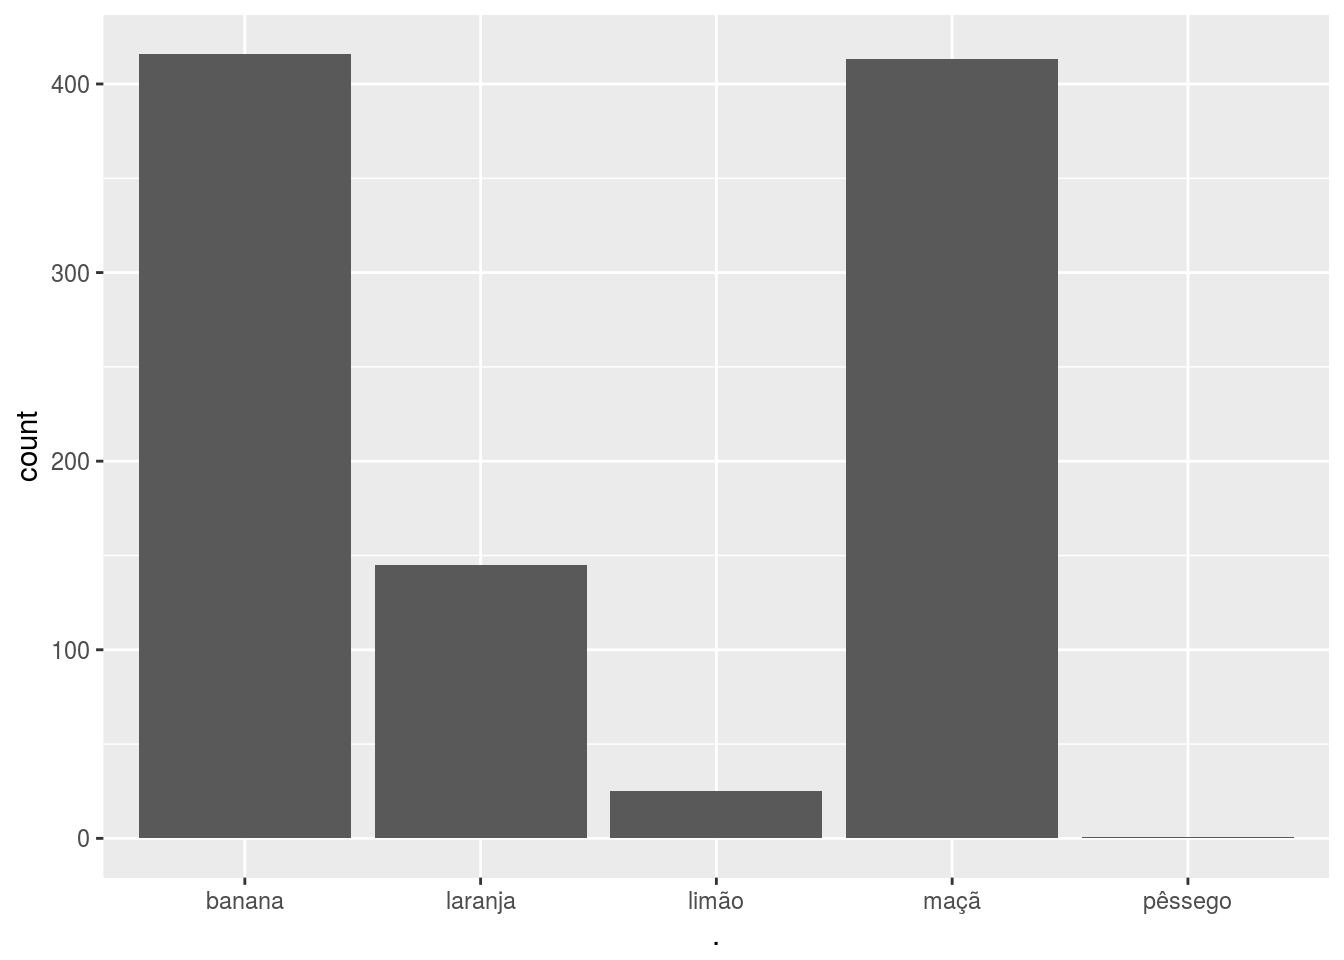
\includegraphics[width=0.5\linewidth]{ragmatic_files/figure-latex/unnamed-chunk-39-1} \end{center}

Note que o eixo \texttt{x} está ordenado alfabeticamente. Como a ordem
das frutas não importa (pois é uma variável nominal), faz mais sentido
ordenarmos as barras de acordo com a quantidade de frutas. Isso é feito
com a função \texttt{fct\_infreq}:

\begin{Shaded}
\begin{Highlighting}[]
\KeywordTok{library}\NormalTok{(forcats)}
\NormalTok{labs %>%}\StringTok{ }\KeywordTok{fct_infreq}\NormalTok{() %>%}\StringTok{ }\NormalTok{ggplot2::}\KeywordTok{qplot}\NormalTok{()}
\end{Highlighting}
\end{Shaded}

\begin{center}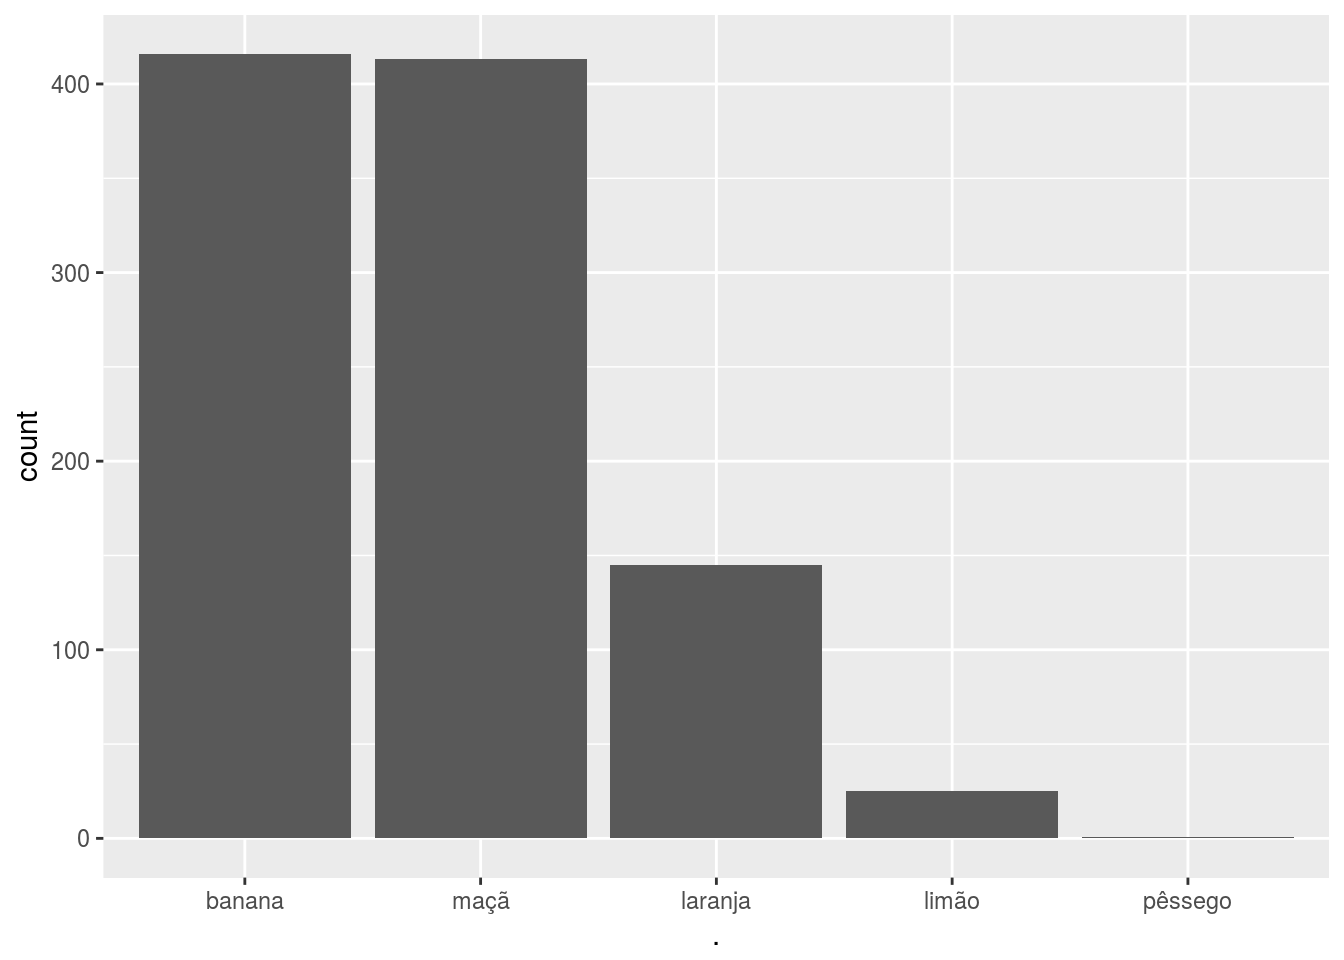
\includegraphics[width=0.5\linewidth]{ragmatic_files/figure-latex/unnamed-chunk-40-1} \end{center}

Outra importante função do \texttt{forcats} possibilita agrupar fatores
de forma eficiente:

\begin{Shaded}
\begin{Highlighting}[]
\NormalTok{labs %>%}\StringTok{ }
\StringTok{  }\KeywordTok{fct_collapse}\NormalTok{(cí}\DataTypeTok{trica =} \KeywordTok{c}\NormalTok{(}\StringTok{'laranja'}\NormalTok{, }\StringTok{'limão'}\NormalTok{)) %>%}\StringTok{ }
\StringTok{  }\KeywordTok{fct_infreq}\NormalTok{() %>%}\StringTok{ }
\StringTok{  }\NormalTok{ggplot2::}\KeywordTok{qplot}\NormalTok{()}
\end{Highlighting}
\end{Shaded}

\begin{center}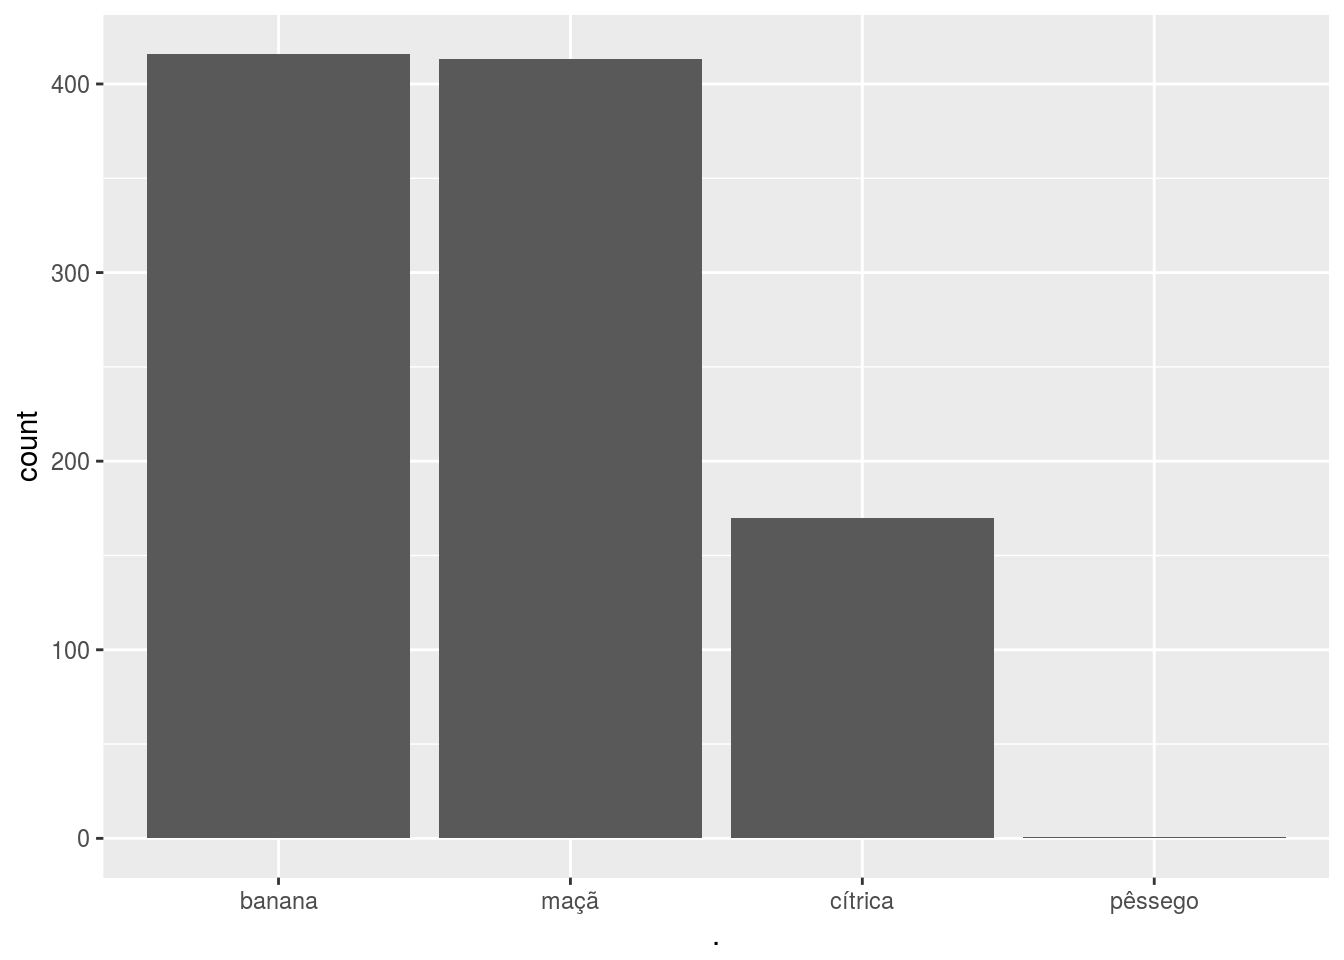
\includegraphics[width=0.5\linewidth]{ragmatic_files/figure-latex/unnamed-chunk-41-1} \end{center}

Outra forma comum de agrupar fatores é agrupar em ``outros'' as
categorias que aparecem poucas vezes na base de dados. Para isso,
utilizamos \texttt{fct\_lump}:

\begin{Shaded}
\begin{Highlighting}[]
\NormalTok{labs %>%}\StringTok{ }\KeywordTok{fct_count}\NormalTok{()}
\end{Highlighting}
\end{Shaded}

\begin{verbatim}
## # A tibble: 5 × 2
##         f     n
##    <fctr> <int>
## 1  banana   416
## 2 laranja   145
## 3   limão    25
## 4    maçã   413
## 5 pêssego     1
\end{verbatim}

\begin{Shaded}
\begin{Highlighting}[]
\CommentTok{# agrupa todas desde que "outro" continue a menor categoria}
\NormalTok{labs %>%}\StringTok{ }\KeywordTok{fct_lump}\NormalTok{(}\DataTypeTok{other_level =} \StringTok{'outros'}\NormalTok{) %>%}\StringTok{ }\NormalTok{ggplot2::}\KeywordTok{qplot}\NormalTok{()}
\CommentTok{# 10% menores}
\NormalTok{labs %>%}\StringTok{ }\KeywordTok{fct_lump}\NormalTok{(}\DataTypeTok{prop =} \NormalTok{.}\DecValTok{10}\NormalTok{, }\DataTypeTok{other_level =} \StringTok{'outros'}\NormalTok{) %>%}\StringTok{ }\NormalTok{ggplot2::}\KeywordTok{qplot}\NormalTok{() }
\CommentTok{# mantém os n maiores}
\NormalTok{labs %>%}\StringTok{ }\KeywordTok{fct_lump}\NormalTok{(}\DataTypeTok{n =} \DecValTok{1}\NormalTok{, }\DataTypeTok{other_level =} \StringTok{'outros'}\NormalTok{) %>%}\StringTok{ }\NormalTok{ggplot2::}\KeywordTok{qplot}\NormalTok{()}
\end{Highlighting}
\end{Shaded}

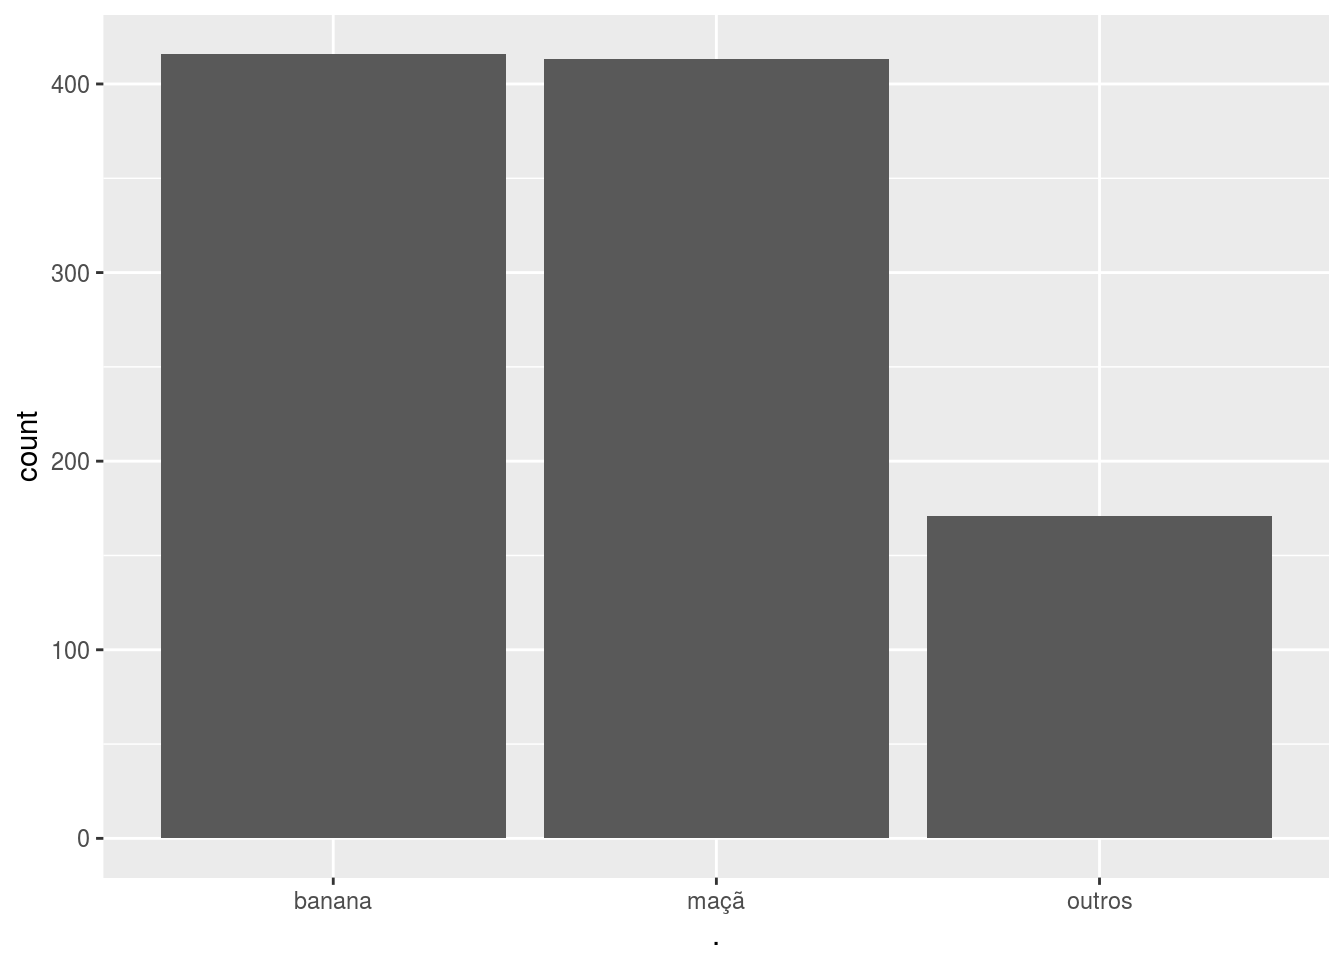
\includegraphics[width=0.33\linewidth]{ragmatic_files/figure-latex/unnamed-chunk-42-1}
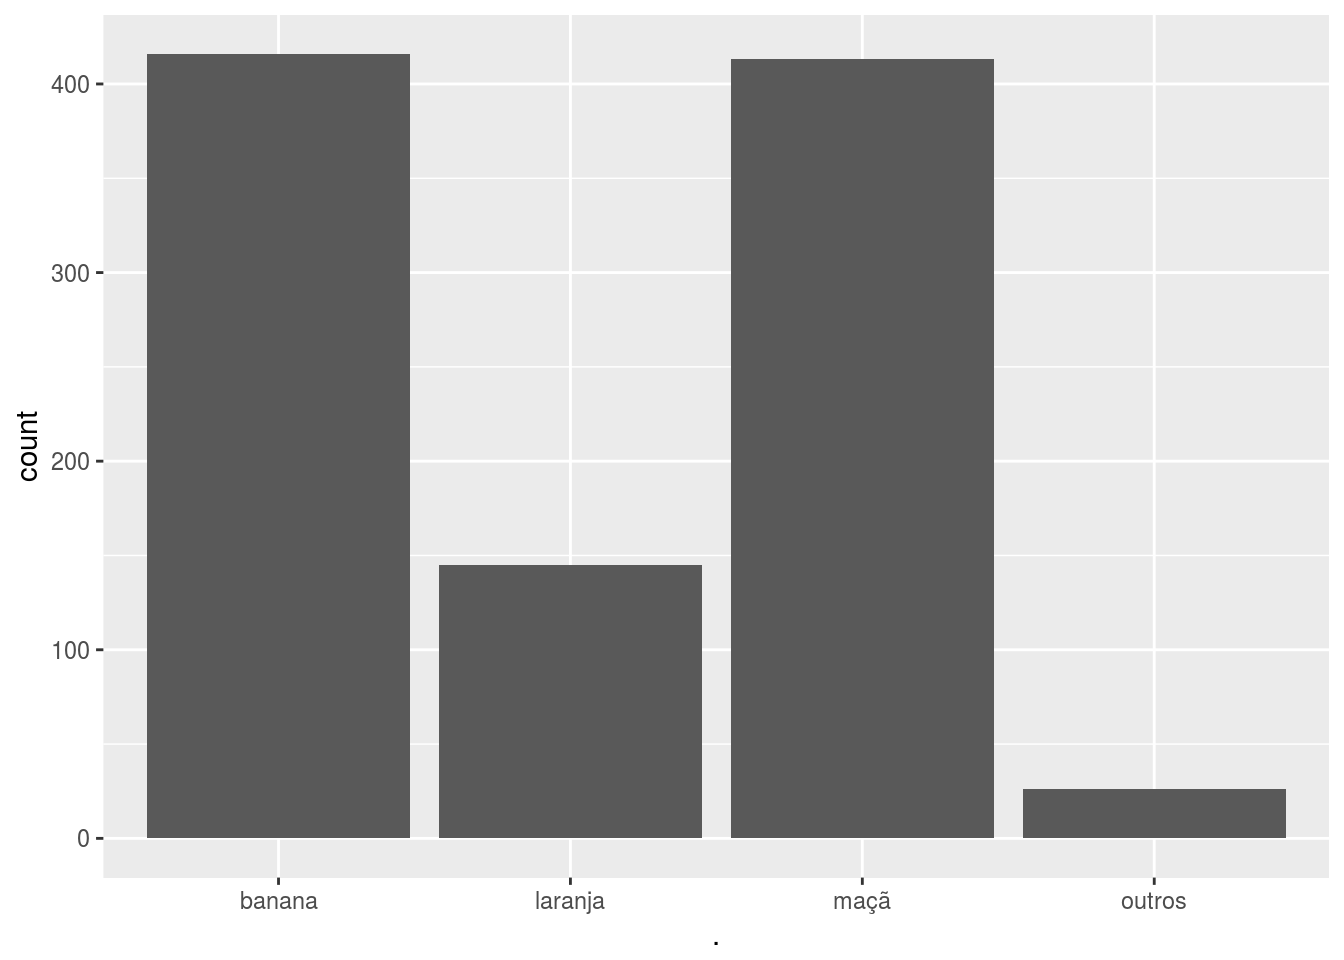
\includegraphics[width=0.33\linewidth]{ragmatic_files/figure-latex/unnamed-chunk-42-2}
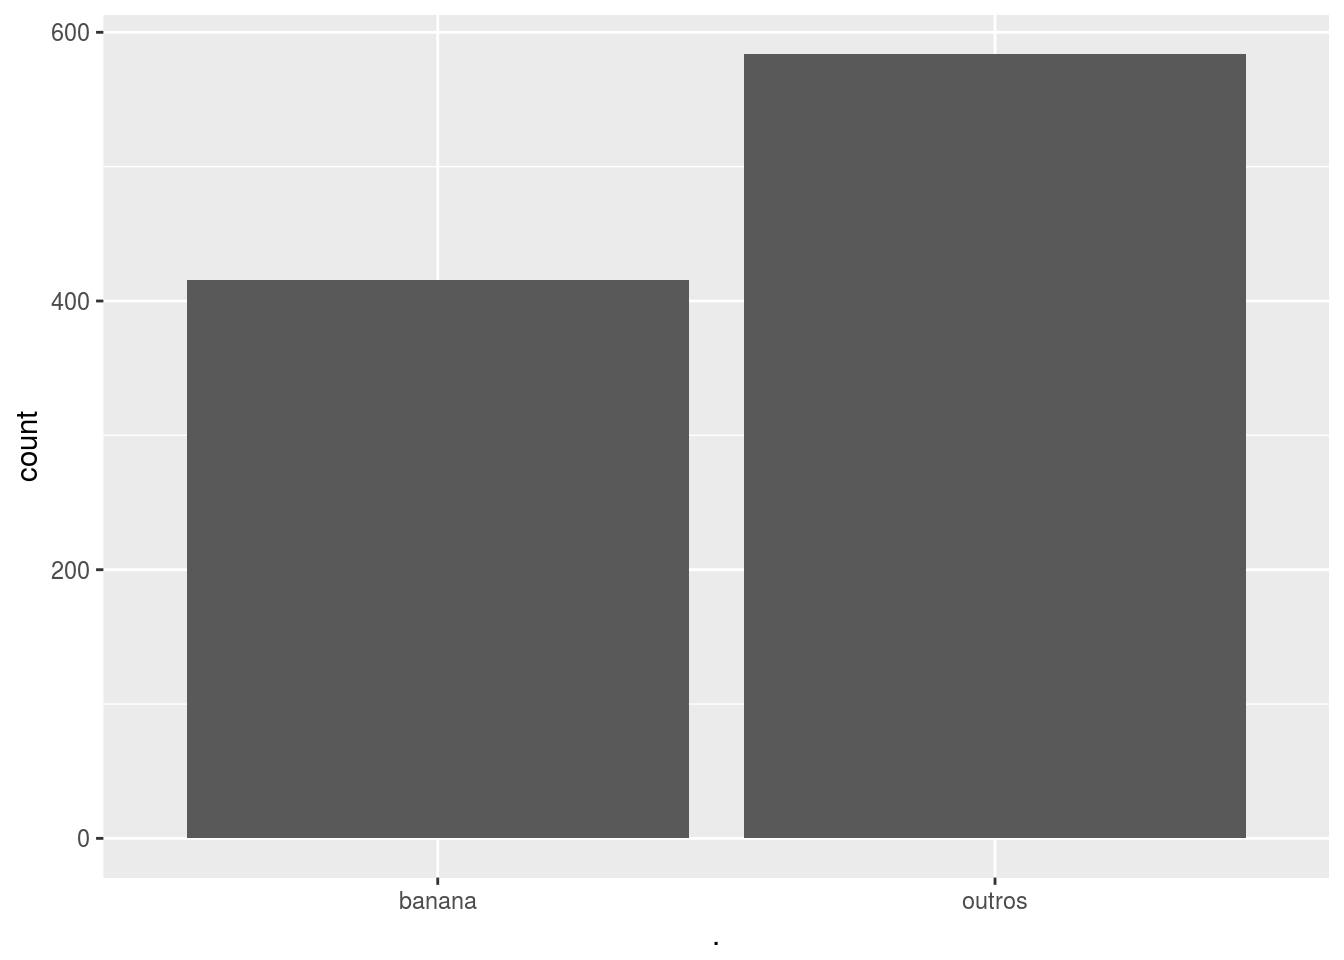
\includegraphics[width=0.33\linewidth]{ragmatic_files/figure-latex/unnamed-chunk-42-3}

Finalmente, uma função útil para produção de gráficos é a
\texttt{fct\_reorder}, que permite utilizar uma variável auxiliar
(possivelmente fazendo sumarizações) para ordenar o fator.

\subsection{Exercício}\label{exercicio-1}

A função \texttt{fct\_reorder} foi utilizada na análise dos inscritos.
Descubra como ela foi utilizada e qual seu efeito no gráfico.

\chapter{Visualização de dados}\label{visualizacao-de-dados}

\section{\texorpdfstring{Com
\texttt{ggplot2}}{Com ggplot2}}\label{com-ggplot2}

O \texttt{ggplot2} é um pacote do R voltado para a criação de gráficos
estatísticos. Ele é baseado na Gramática dos Gráficos (\emph{grammar of
graphics}, em inglês), criado por Leland Wilkinson, que é uma resposta
para a pergunta: o que é um gráfico estatístico? Resumidamente, a
gramática diz que um gráfico estatístico é um mapeamento dos dados a
partir de atributos estéticos (cores, formas, tamanho) em formas
geométricas (pontos, linhas, barras).

Para mais informações sobre a Gramática dos Gráficos, você pode
consultar o livro
\href{http://www.springer.com/statistics/computational+statistics/book/978-0-387-24544-7}{\emph{The
Grammar of graphics}}, escrito pelo Leland Wilkinson, ou o livro
\href{http://ggplot2.org/book/}{ggplot2: elegant graphics for data
analysis}, do Hadley Wickham. Um
\href{http://moderngraphics11.pbworks.com/f/ggplot2-Book09hWickham.pdf}{pdf
do livro} também está disponível.

Parei aqui. Daqui pra baixo está desatualizado!

\subsection{Construindo gráficos}\label{construindo-graficos}

A seguir, vamos discutir os aspcetos básicos para a construção de
gráficos com o pacote \texttt{ggplot2}. Para isso, utilizaremos o banco
de dados contido no objeto \texttt{mtcars}. Para visualizar as primeiras
linhas deste banco, utilize o comando:

\begin{Shaded}
\begin{Highlighting}[]
\KeywordTok{head}\NormalTok{(mtcars)}
\end{Highlighting}
\end{Shaded}

\begin{verbatim}
##                    mpg cyl disp  hp drat    wt  qsec vs am gear carb
## Mazda RX4         21.0   6  160 110 3.90 2.620 16.46  0  1    4    4
## Mazda RX4 Wag     21.0   6  160 110 3.90 2.875 17.02  0  1    4    4
## Datsun 710        22.8   4  108  93 3.85 2.320 18.61  1  1    4    1
## Hornet 4 Drive    21.4   6  258 110 3.08 3.215 19.44  1  0    3    1
## Hornet Sportabout 18.7   8  360 175 3.15 3.440 17.02  0  0    3    2
## Valiant           18.1   6  225 105 2.76 3.460 20.22  1  0    3    1
\end{verbatim}

\subsection{As camadas de um gráfico}\label{as-camadas-de-um-grafico}

No \texttt{ggplot2}, os gráficos são construídos camada por camada (ou,
\emph{layers}, em inglês), sendo que a primeira delas é dada pela função
\texttt{ggplot} (não tem o ``2''). Cada camada representa um tipo de
mapeamento ou personalização do gráfico. O código abaixo é um exemplo de
um gráfico bem simples, construído a partir das duas principais camadas.

\begin{Shaded}
\begin{Highlighting}[]
\KeywordTok{library}\NormalTok{(ggplot2)}
\KeywordTok{ggplot}\NormalTok{(}\DataTypeTok{data =} \NormalTok{mtcars, }\KeywordTok{aes}\NormalTok{(}\DataTypeTok{x =} \NormalTok{disp, }\DataTypeTok{y =} \NormalTok{mpg)) +}\StringTok{ }
\StringTok{  }\KeywordTok{geom_point}\NormalTok{()}
\end{Highlighting}
\end{Shaded}

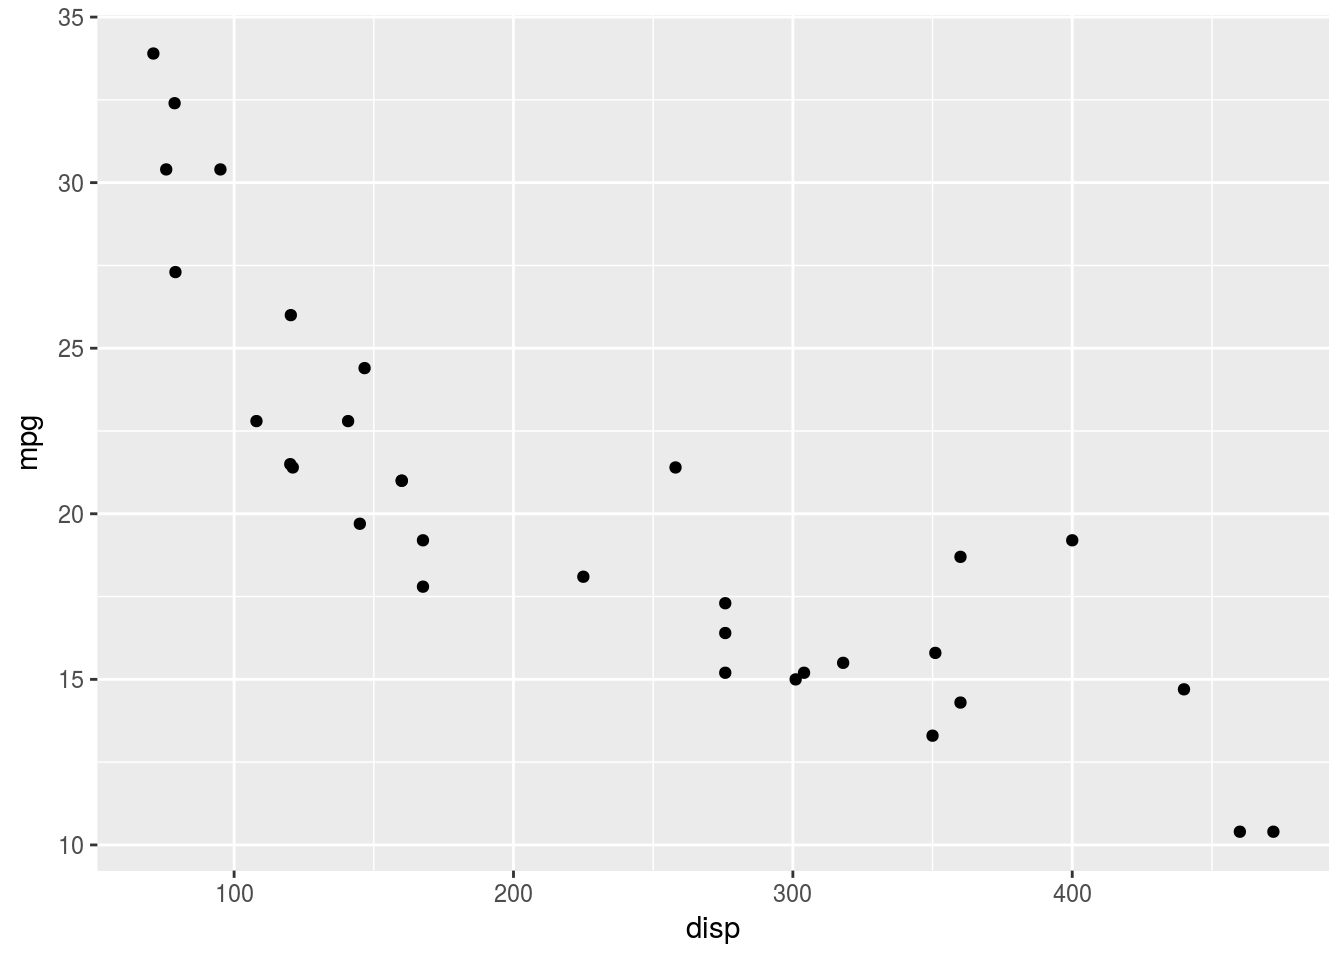
\includegraphics{ragmatic_files/figure-latex/aula05chunk03-1.pdf}

Observe que o primeiro argumento da função \texttt{ggplot} é um data
frame. A função \texttt{aes()} descreve como as variáveis são mapeadas
em aspectos visuais de formas geométricas definidas pelos \emph{geoms}.
Aqui, essas formas geométricas são pontos, selecionados pela função
\texttt{geom\_point()}, gerando, assim, um gráfico de dispersão. A
combinação dessas duas camadas define o tipo de gráfico que você deseja
construir.

\subsubsection{Aesthetics}\label{aesthetics}

A primeira camada de um gráfico deve indicar a relação entre os dados e
cada aspecto visual do gráfico, como qual variável será representada no
eixo x, qual será representada no eixo y, a cor e o tamanho dos
componentes geométricos etc. Os aspectos que podem ou devem ser mapeados
depende do tipo de gráfico que você deseja fazer.

No exemplo acima, atribuímos aspectos de posição: ao eixo y mapeamos a
variável \texttt{mpg} (milhas por galão) e ao eixo x a variável
\texttt{disp} (cilindradas). Outro aspecto que pode ser mapeado nesse
gráfico é a cor dos pontos

\begin{Shaded}
\begin{Highlighting}[]
\KeywordTok{ggplot}\NormalTok{(}\DataTypeTok{data =} \NormalTok{mtcars, }\KeywordTok{aes}\NormalTok{(}\DataTypeTok{x =} \NormalTok{disp, }\DataTypeTok{y =} \NormalTok{mpg, }\DataTypeTok{colour =} \KeywordTok{as.factor}\NormalTok{(am))) +}\StringTok{ }
\StringTok{  }\KeywordTok{geom_point}\NormalTok{()}
\end{Highlighting}
\end{Shaded}

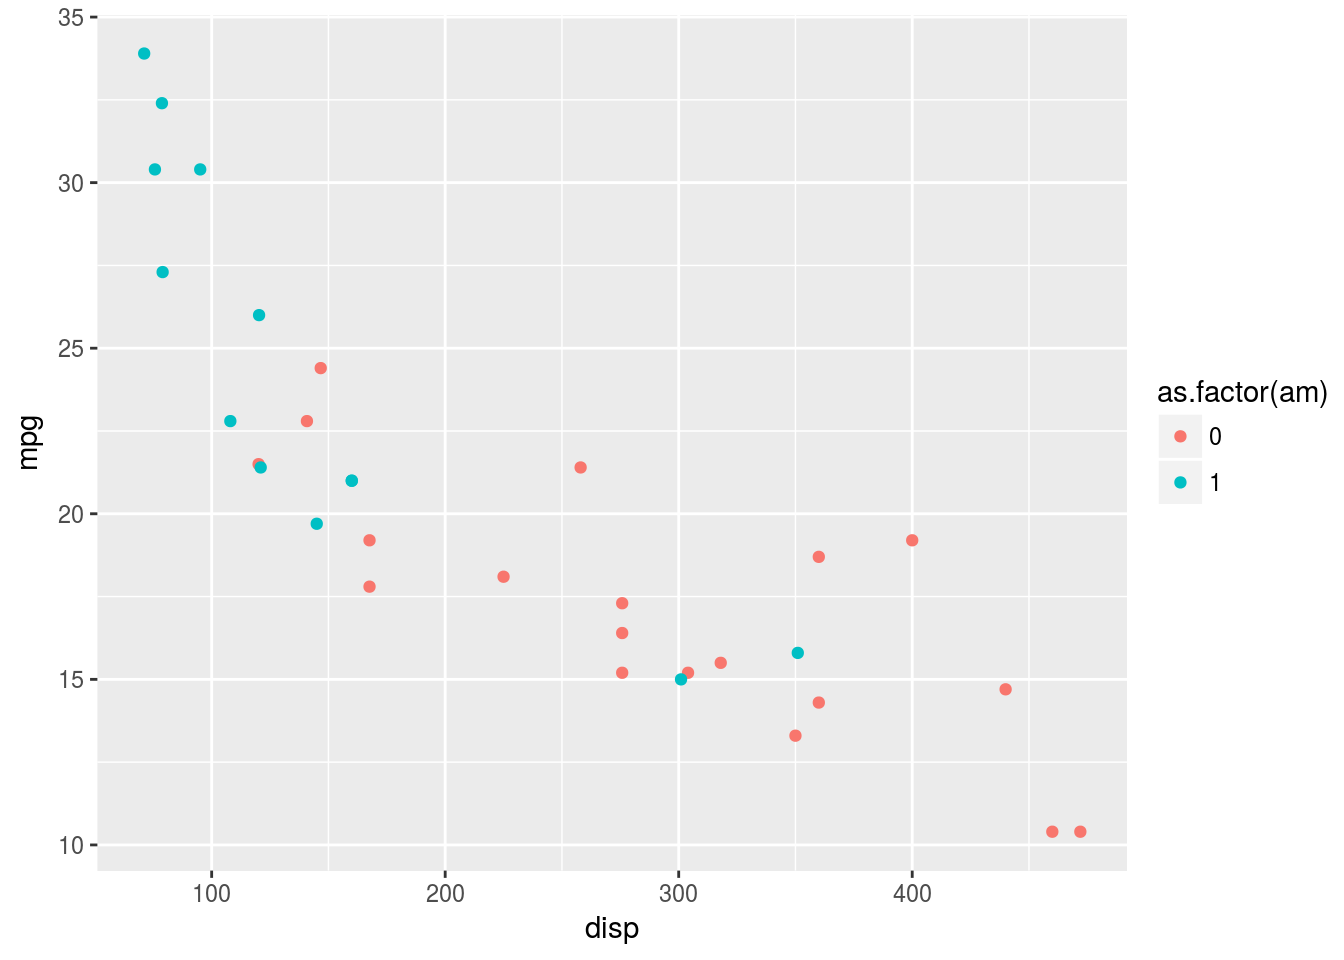
\includegraphics{ragmatic_files/figure-latex/aula05chunk04-1.pdf}

Agora, a variável \texttt{am} (tipo de transmissão) foi mapeada à cor
dos pontos, sendo que pontos vermelhos correspondem à transmissão
automática (valor 0) e pontos azuis à transmissão manual (valor 1).
Observe que inserimos a variável \texttt{am} como um fator, pois temos
interesse apenas nos valores ``0'' e ``1''. No entanto, tambem podemos
mapear uma variável contínua à cor dos pontos:

\begin{Shaded}
\begin{Highlighting}[]
\KeywordTok{ggplot}\NormalTok{(mtcars, }\KeywordTok{aes}\NormalTok{(}\DataTypeTok{x =} \NormalTok{disp, }\DataTypeTok{y =} \NormalTok{mpg, }\DataTypeTok{colour =} \NormalTok{cyl)) +}\StringTok{ }
\StringTok{  }\KeywordTok{geom_point}\NormalTok{()}
\end{Highlighting}
\end{Shaded}

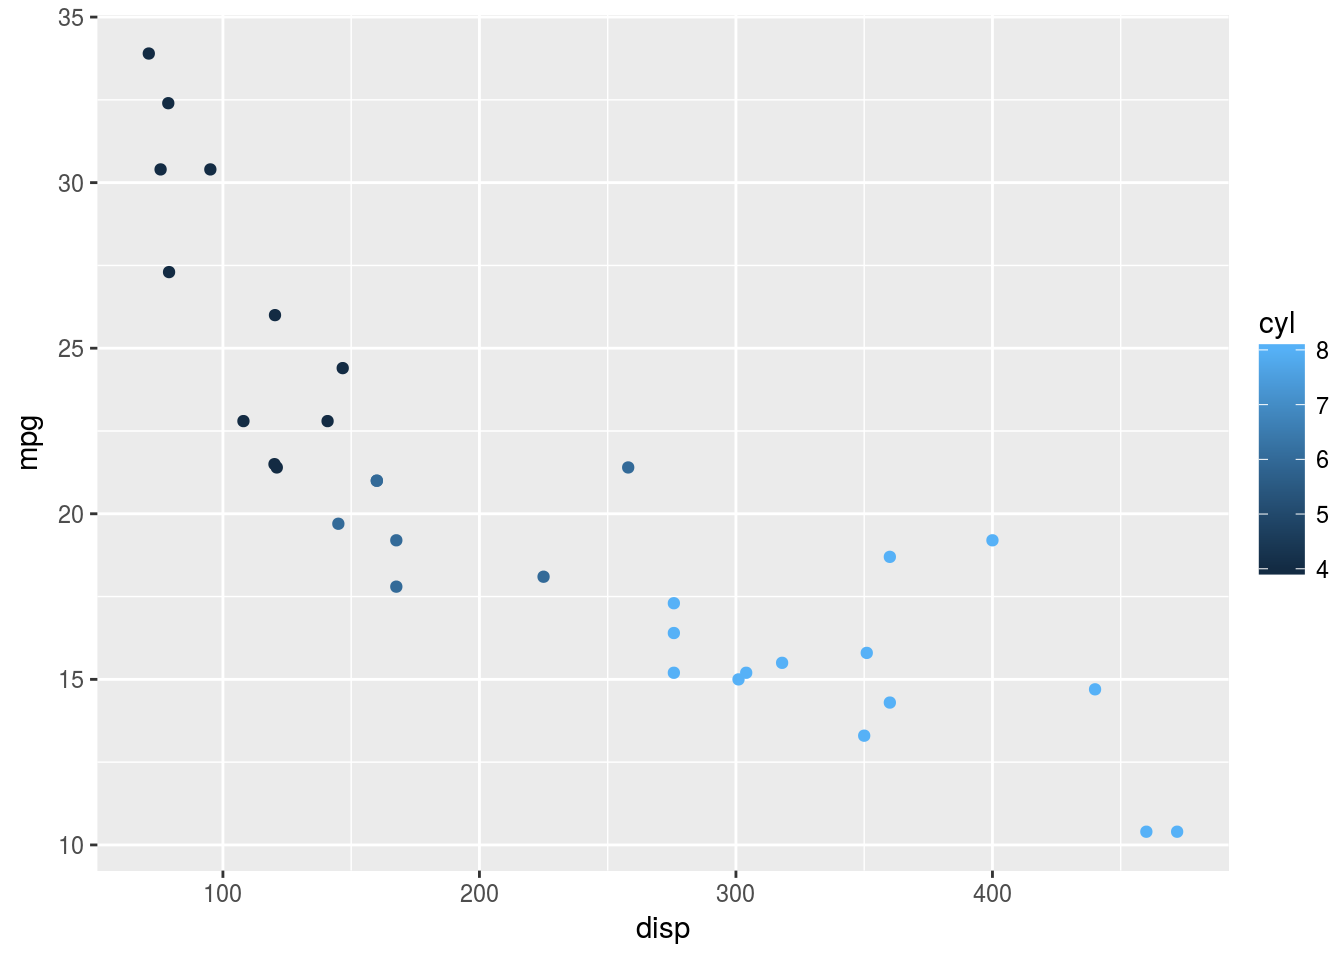
\includegraphics{ragmatic_files/figure-latex/aula05chunk05-1.pdf}

Aqui, o número de cilindros, \texttt{cyl}, é representado pela
tonalidade da cor azul.

\textbf{Nota}: por \emph{default}, a legenda é insirida no gráfico
automaticamente.

Também podemos mapear o tamanho dos pontos à uma variável de interesse:

\begin{Shaded}
\begin{Highlighting}[]
\KeywordTok{ggplot}\NormalTok{(mtcars, }\KeywordTok{aes}\NormalTok{(}\DataTypeTok{x =} \NormalTok{disp, }\DataTypeTok{y =} \NormalTok{mpg, }\DataTypeTok{colour =} \NormalTok{cyl, }\DataTypeTok{size =} \NormalTok{wt)) +}
\StringTok{  }\KeywordTok{geom_point}\NormalTok{()}
\end{Highlighting}
\end{Shaded}

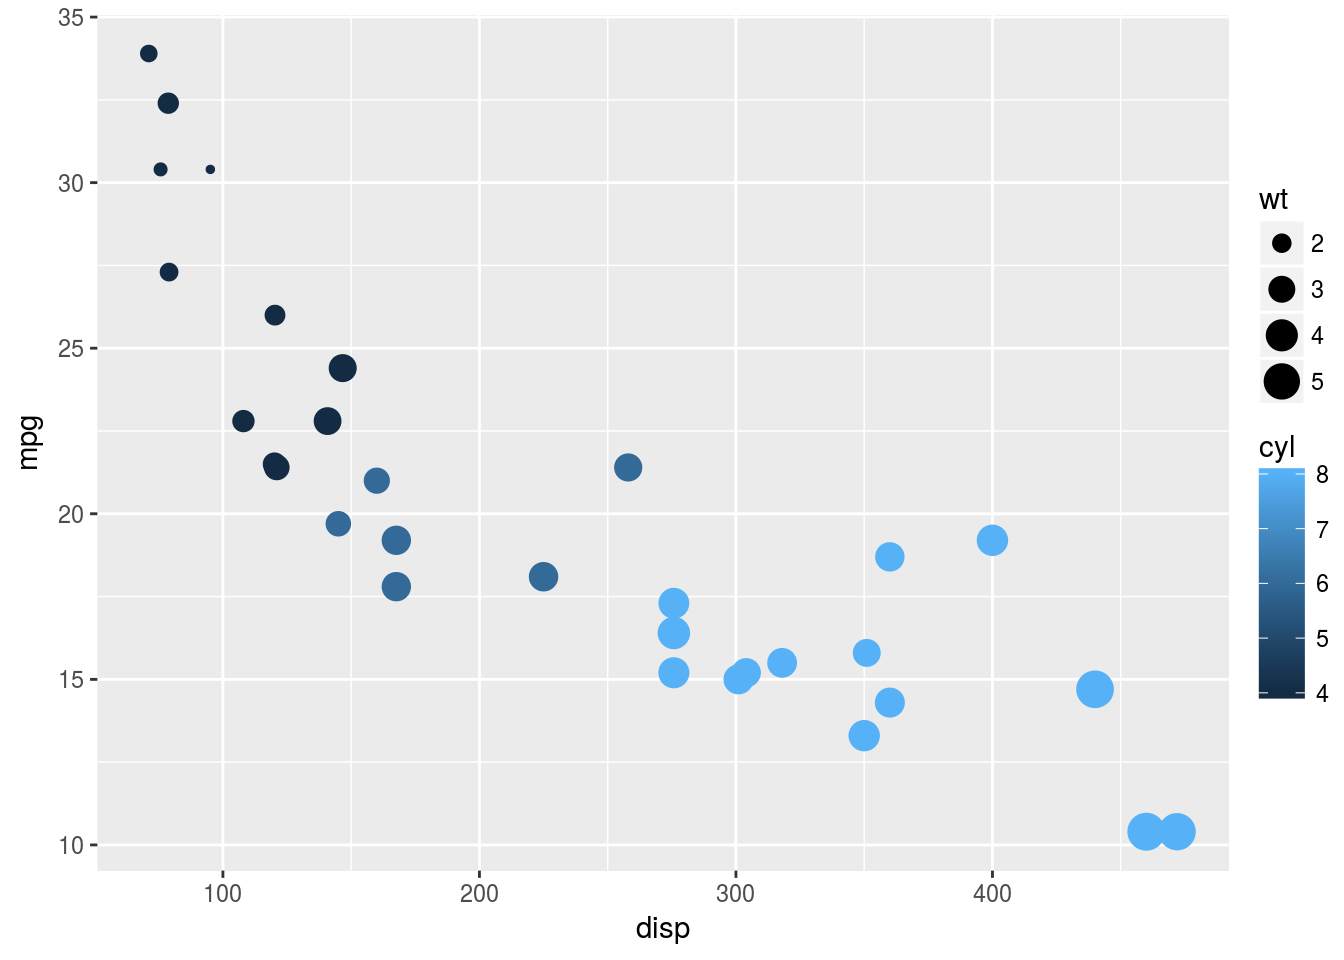
\includegraphics{ragmatic_files/figure-latex/aula05chunk06-1.pdf}

\textbf{Exercício}: pesquisar mais aspectos que podem ser alterados no
gráfico de dispersão.

\subsubsection{Geoms}\label{geoms}

Os \emph{geoms} definem qual forma geométrica será utilizada para a
visualização dos dados no gráfico. Como já vimos, a função
\texttt{geom\_point()} gera gráficos de dispersão transformando pares
(x,y) em pontos. Veja a seguir outros \emph{geoms} bastante utilizados:

\begin{itemize}
\tightlist
\item
  geom\_line: para retas definidas por pares (x,y)
\item
  geom\_abline: para retas definidas por um intercepto e uma inclinação
\item
  geom\_hline: para retas horizontais
\item
  geom\_boxplot: para boxplots
\item
  geom\_histogram: para histogramas
\item
  geom\_density: para densidades
\item
  geom\_area: para áreas
\item
  geom\_bar: para barras
\end{itemize}

Veja a seguir como é fácil gerar diversos gráficos diferentes utilizando
a mesma estrutura do gráfico de dispersão acima:

\begin{Shaded}
\begin{Highlighting}[]
\KeywordTok{ggplot}\NormalTok{(mtcars, }\KeywordTok{aes}\NormalTok{(}\DataTypeTok{x =} \KeywordTok{as.factor}\NormalTok{(cyl), }\DataTypeTok{y =} \NormalTok{mpg)) +}\StringTok{ }
\StringTok{  }\KeywordTok{geom_boxplot}\NormalTok{()}
\end{Highlighting}
\end{Shaded}

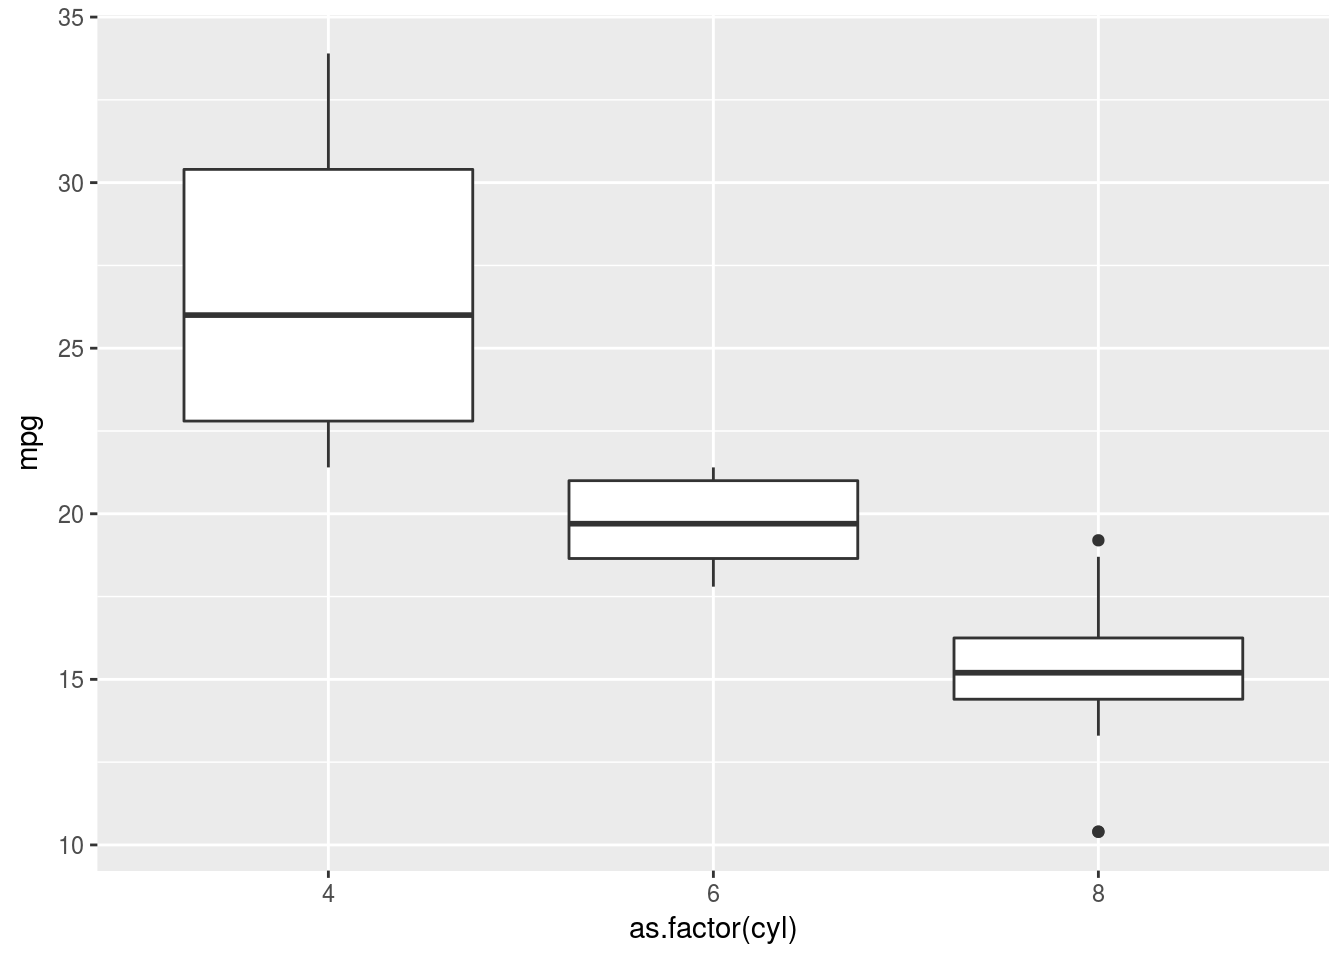
\includegraphics{ragmatic_files/figure-latex/aula05chunk07-1.pdf}

\begin{Shaded}
\begin{Highlighting}[]
\KeywordTok{ggplot}\NormalTok{(mtcars, }\KeywordTok{aes}\NormalTok{(}\DataTypeTok{x =} \NormalTok{mpg)) +}\StringTok{ }
\StringTok{  }\KeywordTok{geom_histogram}\NormalTok{()}
\end{Highlighting}
\end{Shaded}

\begin{verbatim}
## `stat_bin()` using `bins = 30`. Pick better value with `binwidth`.
\end{verbatim}

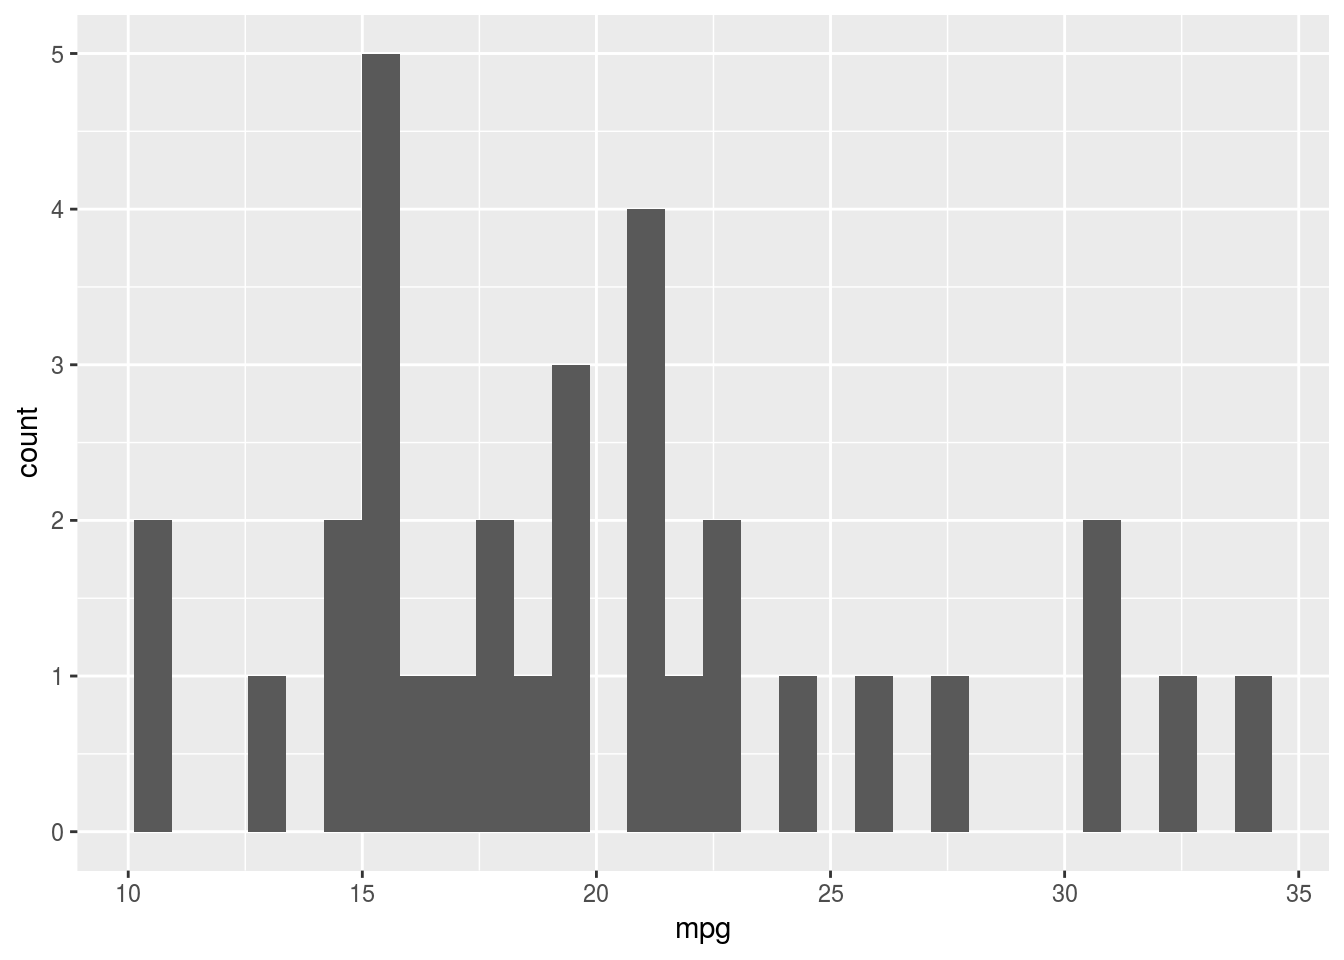
\includegraphics{ragmatic_files/figure-latex/aula05chunk08-1.pdf}

\begin{Shaded}
\begin{Highlighting}[]
\KeywordTok{ggplot}\NormalTok{(mtcars, }\KeywordTok{aes}\NormalTok{(}\DataTypeTok{x =} \KeywordTok{as.factor}\NormalTok{(cyl))) +}\StringTok{ }
\StringTok{  }\KeywordTok{geom_bar}\NormalTok{()}
\end{Highlighting}
\end{Shaded}

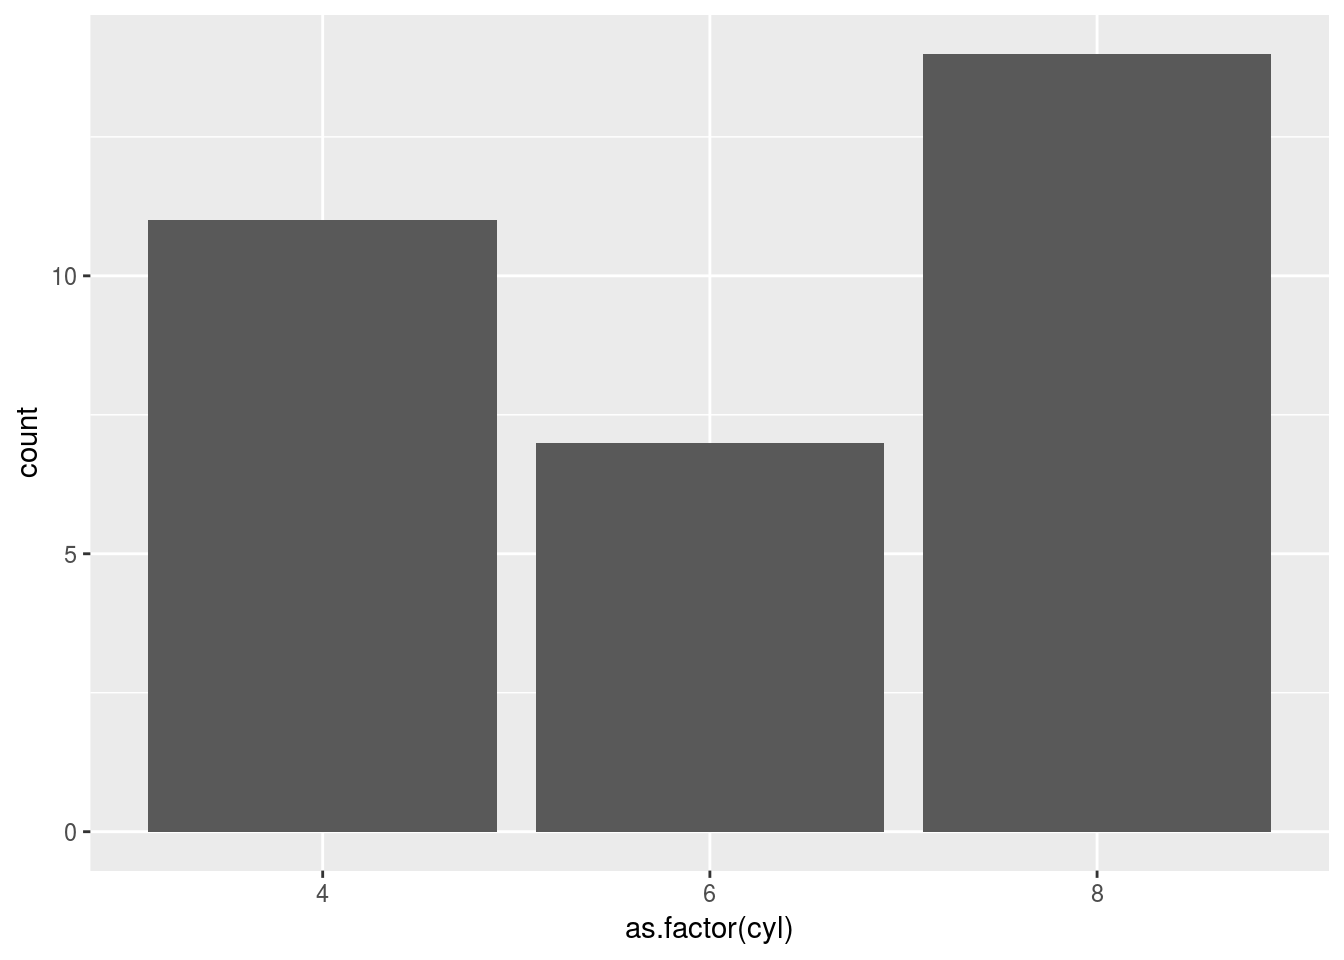
\includegraphics{ragmatic_files/figure-latex/aula05chunk09-1.pdf}

Para fazer um boxplot para cada grupo, precisamos passar para o aspecto
x do gráfico uma variável do tipo fator. \#\#\# Personalizando os
gráficos

\subsubsection{Cores}\label{cores}

O aspecto colour do boxplot, muda a cor do contorno. Para mudar o
preenchimento, basta usar o \texttt{fill}.

\begin{Shaded}
\begin{Highlighting}[]
\KeywordTok{ggplot}\NormalTok{(mtcars, }\KeywordTok{aes}\NormalTok{(}\DataTypeTok{x =} \KeywordTok{as.factor}\NormalTok{(cyl), }\DataTypeTok{y =} \NormalTok{mpg, }\DataTypeTok{colour =} \KeywordTok{as.factor}\NormalTok{(cyl))) +}\StringTok{ }
\StringTok{  }\KeywordTok{geom_boxplot}\NormalTok{()}
\end{Highlighting}
\end{Shaded}

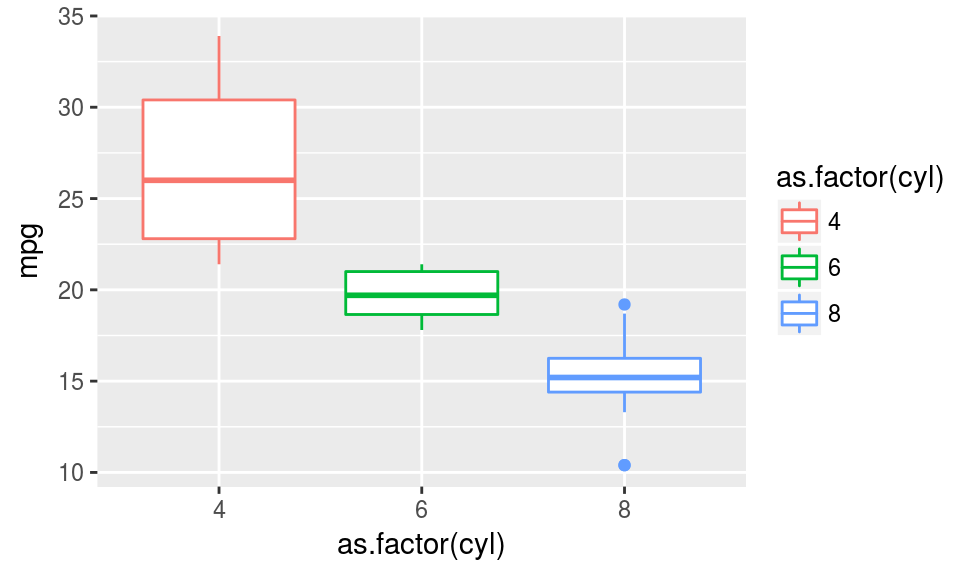
\includegraphics{ragmatic_files/figure-latex/aula05chunk10-1.pdf}

\begin{Shaded}
\begin{Highlighting}[]
\KeywordTok{ggplot}\NormalTok{(mtcars, }\KeywordTok{aes}\NormalTok{(}\DataTypeTok{x =} \KeywordTok{as.factor}\NormalTok{(cyl), }\DataTypeTok{y =} \NormalTok{mpg, }\DataTypeTok{fill =} \KeywordTok{as.factor}\NormalTok{(cyl))) +}\StringTok{ }\KeywordTok{geom_boxplot}\NormalTok{()}
\end{Highlighting}
\end{Shaded}

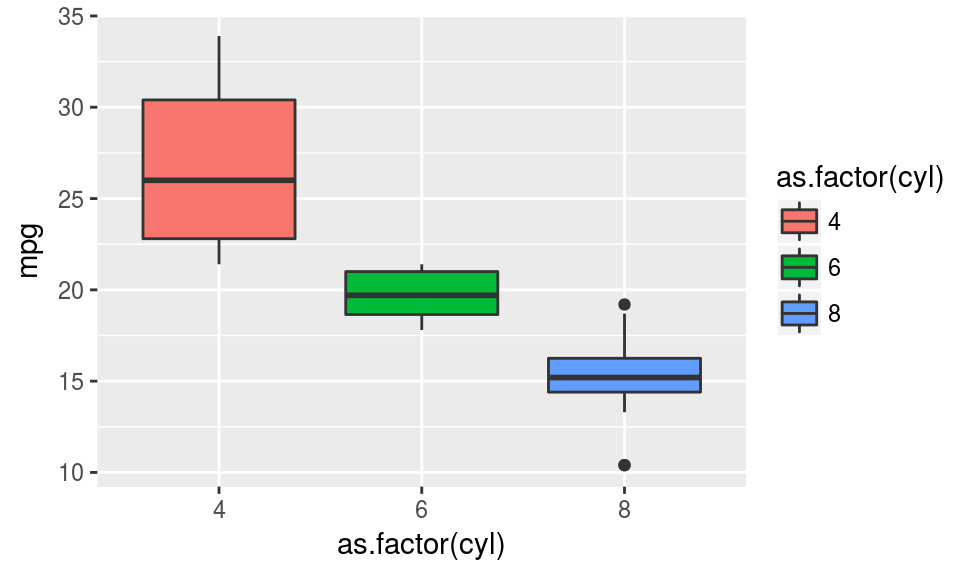
\includegraphics{ragmatic_files/figure-latex/aula05chunk11-1.pdf}

Você pode também mudar a cor dos objetos sem mapeá-la a uma variável.
Para isso, observe que os aspectos \texttt{colour} e \texttt{fill} são
especificados fora do \texttt{aes()}.

\begin{Shaded}
\begin{Highlighting}[]
\KeywordTok{ggplot}\NormalTok{(mtcars, }\KeywordTok{aes}\NormalTok{(}\DataTypeTok{x =} \KeywordTok{as.factor}\NormalTok{(cyl), }\DataTypeTok{y =} \NormalTok{mpg)) +}\StringTok{ }
\StringTok{  }\KeywordTok{geom_boxplot}\NormalTok{(}\DataTypeTok{color =} \StringTok{"red"}\NormalTok{, }\DataTypeTok{fill =} \StringTok{"pink"}\NormalTok{)}
\end{Highlighting}
\end{Shaded}

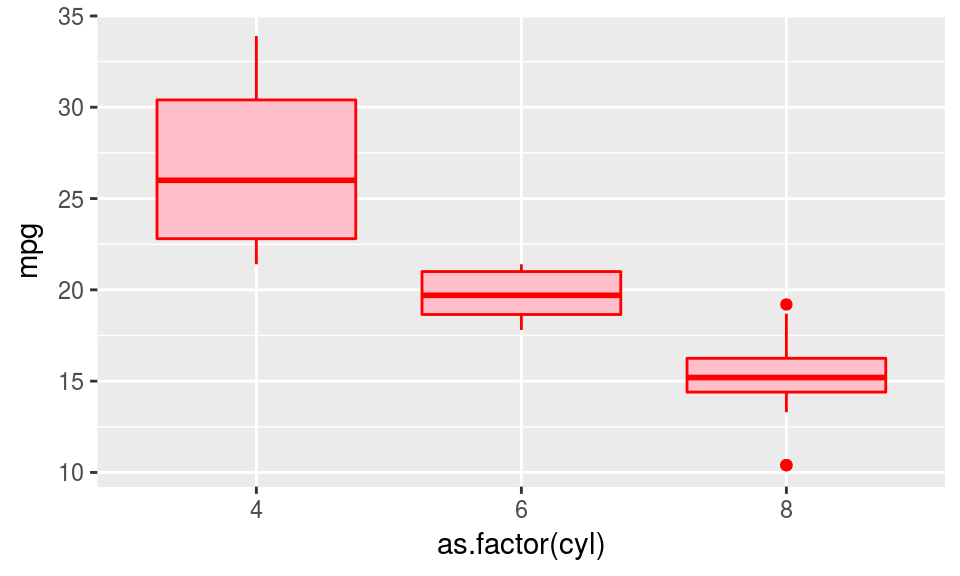
\includegraphics{ragmatic_files/figure-latex/aula05chunk12-1.pdf}

\subsubsection{Eixos}\label{eixos}

Para alterar os labels dos eixos acrescentamos as funções
\texttt{xlab()} ou \texttt{ylab()}.

\begin{Shaded}
\begin{Highlighting}[]
\KeywordTok{ggplot}\NormalTok{(mtcars, }\KeywordTok{aes}\NormalTok{(}\DataTypeTok{x =} \NormalTok{mpg)) +}\StringTok{ }
\StringTok{  }\KeywordTok{geom_histogram}\NormalTok{() +}
\StringTok{  }\KeywordTok{xlab}\NormalTok{(}\StringTok{"Milhas por galão"}\NormalTok{) +}
\StringTok{  }\KeywordTok{ylab}\NormalTok{(}\StringTok{"Frequência"}\NormalTok{)}
\end{Highlighting}
\end{Shaded}

\begin{verbatim}
## `stat_bin()` using `bins = 30`. Pick better value with `binwidth`.
\end{verbatim}

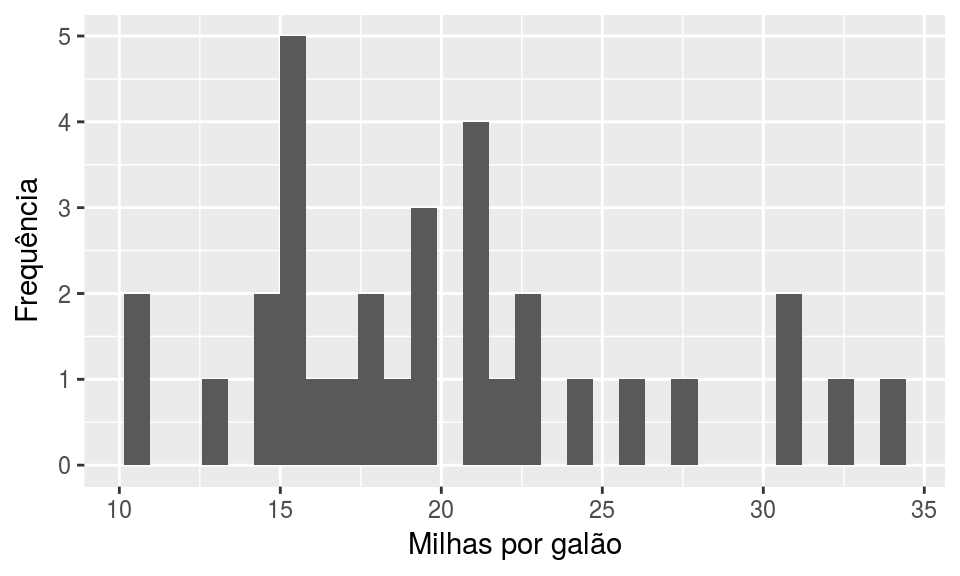
\includegraphics{ragmatic_files/figure-latex/aula05chunk13-1.pdf}

Para alterar os limites dos gráficos usamos as funções \texttt{xlim()} e
\texttt{ylim()}.

\begin{Shaded}
\begin{Highlighting}[]
\KeywordTok{ggplot}\NormalTok{(mtcars, }\KeywordTok{aes}\NormalTok{(}\DataTypeTok{x =} \NormalTok{mpg)) +}\StringTok{ }
\StringTok{  }\KeywordTok{geom_histogram}\NormalTok{() +}
\StringTok{  }\KeywordTok{xlab}\NormalTok{(}\StringTok{"Milhas por galão"}\NormalTok{) +}
\StringTok{  }\KeywordTok{ylab}\NormalTok{(}\StringTok{"Frequência"}\NormalTok{) +}
\StringTok{  }\KeywordTok{xlim}\NormalTok{(}\KeywordTok{c}\NormalTok{(}\DecValTok{0}\NormalTok{, }\DecValTok{40}\NormalTok{)) +}
\StringTok{  }\KeywordTok{ylim}\NormalTok{(}\KeywordTok{c}\NormalTok{(}\DecValTok{0}\NormalTok{,}\DecValTok{8}\NormalTok{))}
\end{Highlighting}
\end{Shaded}

\begin{verbatim}
## `stat_bin()` using `bins = 30`. Pick better value with `binwidth`.
\end{verbatim}

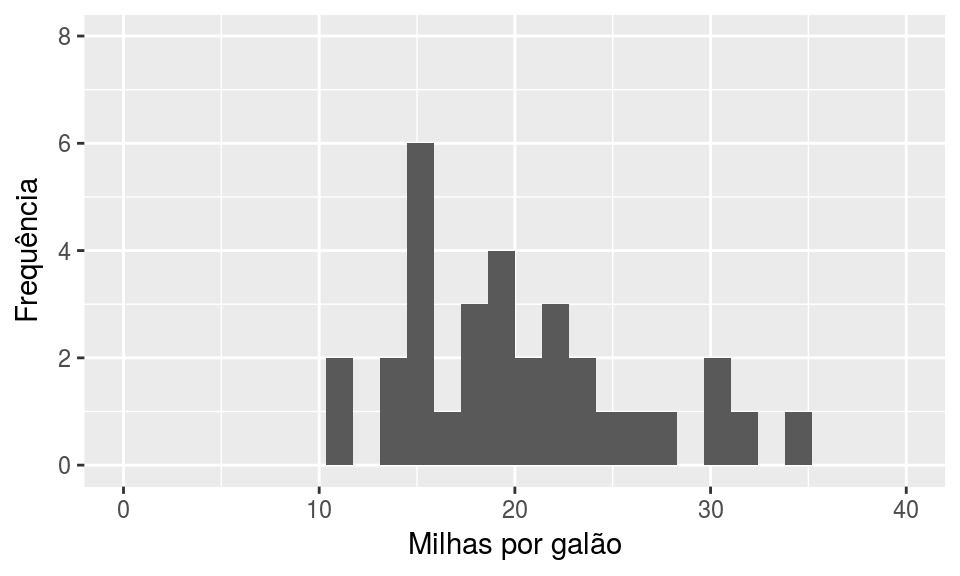
\includegraphics{ragmatic_files/figure-latex/aula05chunk14-1.pdf}

\subsubsection{Legendas}\label{legendas}

A legenda de um gráfico pode ser facilmente personalizada.

Para trocar o \emph{label} da leganda:

\begin{Shaded}
\begin{Highlighting}[]
\KeywordTok{ggplot}\NormalTok{(mtcars, }\KeywordTok{aes}\NormalTok{(}\DataTypeTok{x =} \KeywordTok{as.factor}\NormalTok{(cyl), }\DataTypeTok{fill =} \KeywordTok{as.factor}\NormalTok{(cyl))) +}\StringTok{ }
\StringTok{  }\KeywordTok{geom_bar}\NormalTok{() +}
\StringTok{  }\KeywordTok{labs}\NormalTok{(}\DataTypeTok{fill =} \StringTok{"cyl"}\NormalTok{)}
\end{Highlighting}
\end{Shaded}

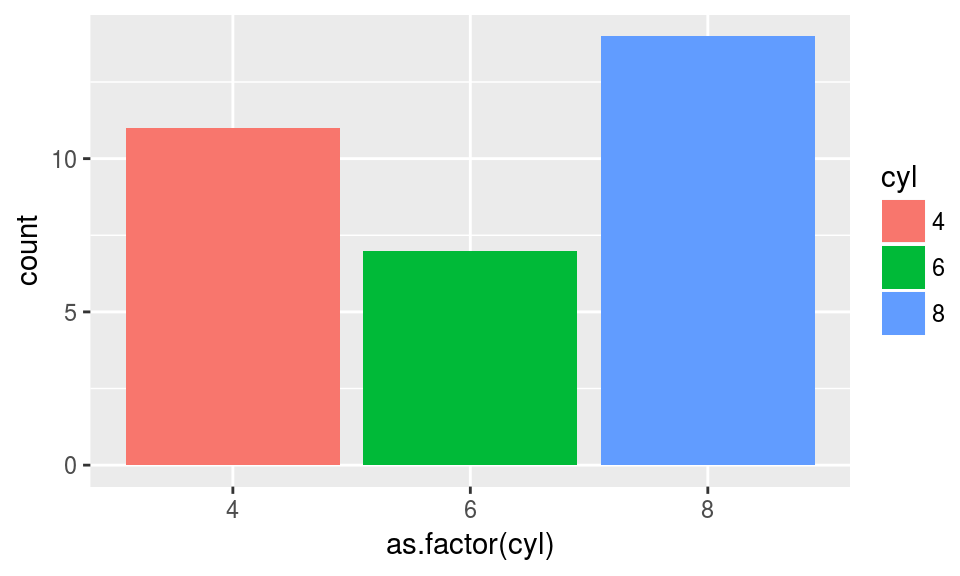
\includegraphics{ragmatic_files/figure-latex/aula05chunk15-1.pdf}

Para trocar a posição da legenda:

\begin{Shaded}
\begin{Highlighting}[]
\KeywordTok{ggplot}\NormalTok{(mtcars, }\KeywordTok{aes}\NormalTok{(}\DataTypeTok{x =} \KeywordTok{as.factor}\NormalTok{(cyl), }\DataTypeTok{fill =} \KeywordTok{as.factor}\NormalTok{(cyl))) +}\StringTok{ }
\StringTok{  }\KeywordTok{geom_bar}\NormalTok{() +}
\StringTok{  }\KeywordTok{labs}\NormalTok{(}\DataTypeTok{fill =} \StringTok{"cyl"}\NormalTok{) +}
\StringTok{  }\KeywordTok{theme}\NormalTok{(}\DataTypeTok{legend.position=}\StringTok{"top"}\NormalTok{)}
\end{Highlighting}
\end{Shaded}

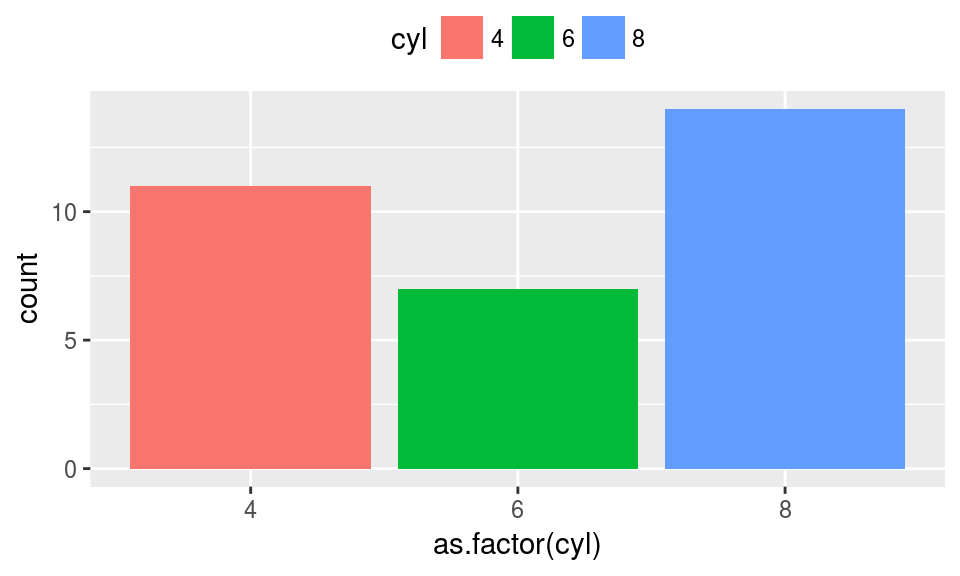
\includegraphics{ragmatic_files/figure-latex/aula05chunk16-1.pdf}

Para retirar a legenda:

\begin{Shaded}
\begin{Highlighting}[]
\KeywordTok{ggplot}\NormalTok{(mtcars, }\KeywordTok{aes}\NormalTok{(}\DataTypeTok{x =} \KeywordTok{as.factor}\NormalTok{(cyl), }\DataTypeTok{fill =} \KeywordTok{as.factor}\NormalTok{(cyl))) +}\StringTok{ }
\StringTok{  }\KeywordTok{geom_bar}\NormalTok{() +}
\StringTok{  }\KeywordTok{guides}\NormalTok{(}\DataTypeTok{fill=}\OtherTok{FALSE}\NormalTok{)}
\end{Highlighting}
\end{Shaded}

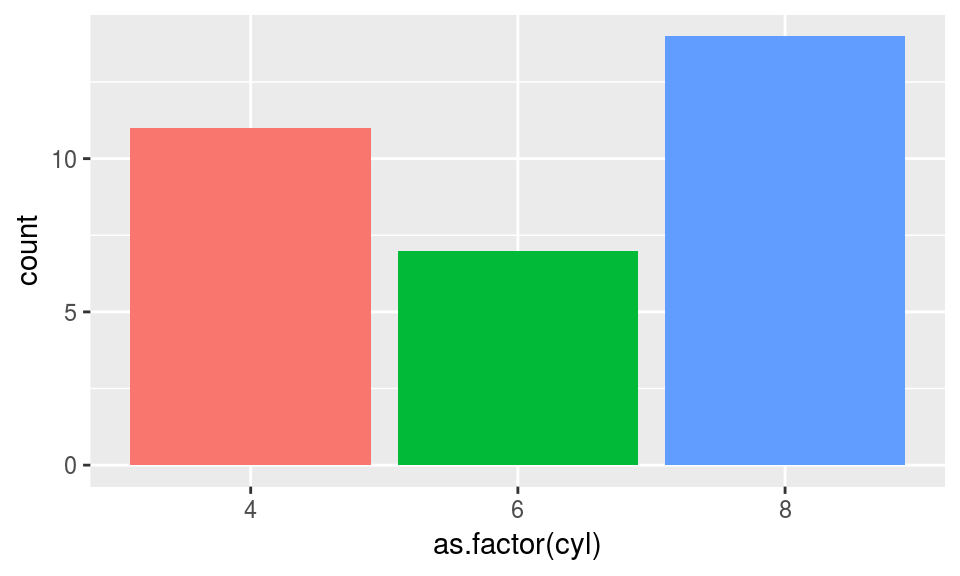
\includegraphics{ragmatic_files/figure-latex/aula05chunk17-1.pdf}

Veja mais opções de personalização
\href{http://www.cookbook-r.com/Graphs/Legends_(ggplot2)/}{aqui!}

\subsubsection{Facets}\label{facets}

Outra funcionalidade muito importante do ggplot é o uso de
\emph{facets}.

\begin{Shaded}
\begin{Highlighting}[]
\KeywordTok{ggplot}\NormalTok{(mtcars, }\KeywordTok{aes}\NormalTok{(}\DataTypeTok{x =} \NormalTok{mpg, }\DataTypeTok{y =} \NormalTok{disp, }\DataTypeTok{colour =} \KeywordTok{as.factor}\NormalTok{(cyl))) +}\StringTok{ }
\StringTok{  }\KeywordTok{geom_point}\NormalTok{() +}\StringTok{ }
\StringTok{  }\KeywordTok{facet_grid}\NormalTok{(am~.)}
\end{Highlighting}
\end{Shaded}

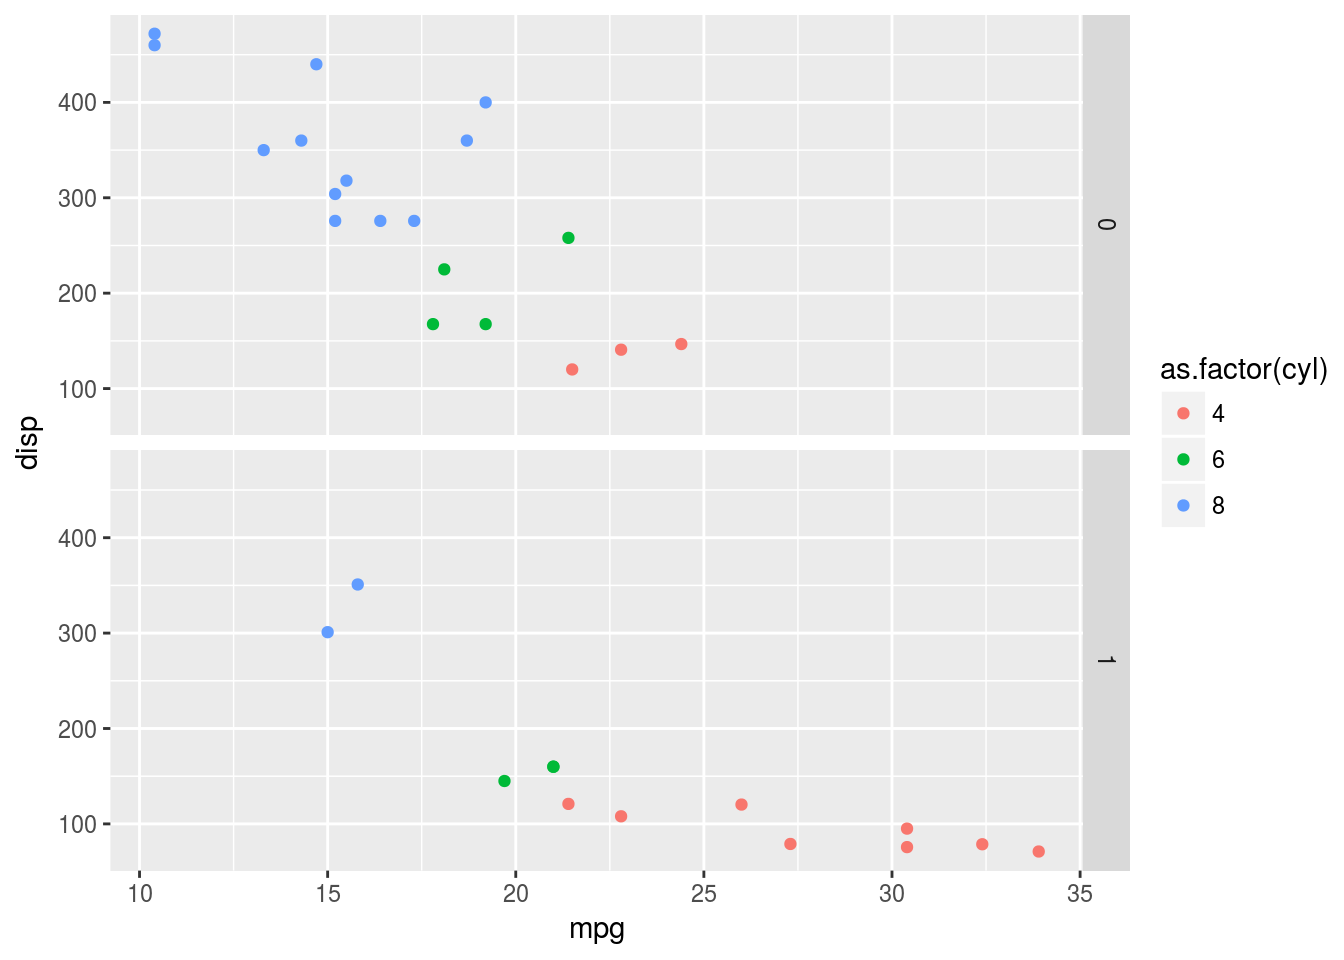
\includegraphics{ragmatic_files/figure-latex/aula05chunk18-1.pdf}

Podemos colocar os graficos lado a lado também:

\begin{Shaded}
\begin{Highlighting}[]
\KeywordTok{ggplot}\NormalTok{(mtcars, }\KeywordTok{aes}\NormalTok{(}\DataTypeTok{x =} \NormalTok{mpg, }\DataTypeTok{y =} \NormalTok{disp, }\DataTypeTok{colour =} \KeywordTok{as.factor}\NormalTok{(cyl))) +}
\StringTok{  }\KeywordTok{geom_point}\NormalTok{() +}\StringTok{ }
\StringTok{  }\KeywordTok{facet_grid}\NormalTok{(.~am)}
\end{Highlighting}
\end{Shaded}

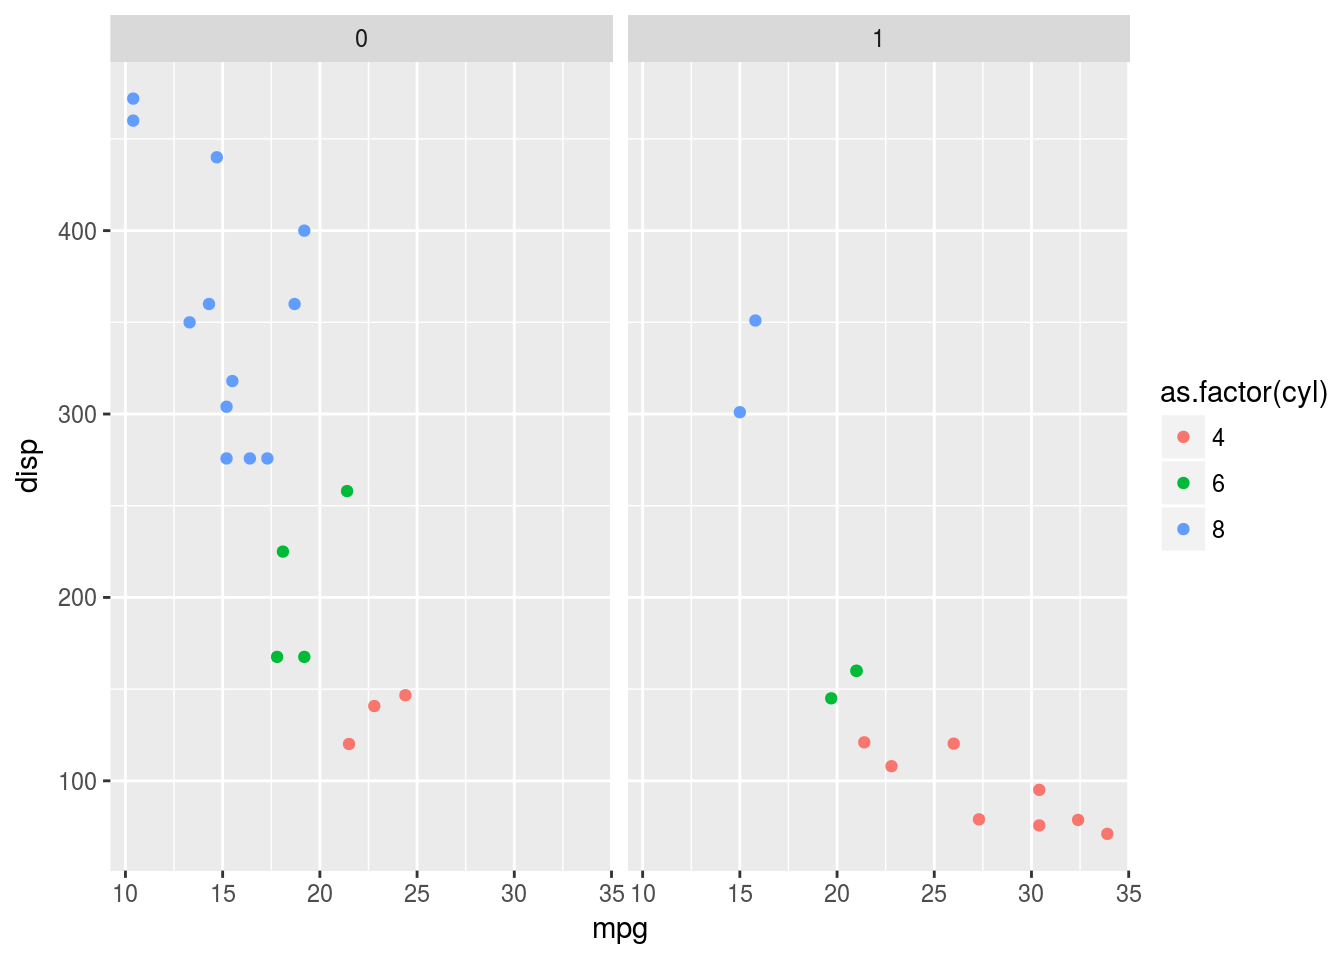
\includegraphics{ragmatic_files/figure-latex/aula05chunk19-1.pdf}

\chapter{Transformação de dados}\label{transformacao-de-dados}

A transformação de dados é uma tarefa usualmente dolorosa e demorada,
podendo tomar a maior parte do tempo da análise. No entanto, como nosso
interesse geralmente é na modelagem dos dados, essa tarefa é muitas
vezes negligenciada.

\begin{quote}
``(\ldots{}) The fact that data science exists as a field is a colossal
failure of statistics. To me, {[}what I do{]} is what statistics is all
about. It is gaining insight from data using modelling and
visualization. Data munging and manipulation is hard and statistics has
just said that's not our domain.''

Hadley Wickham
\end{quote}

\section{\texorpdfstring{Pacotes \texttt{dplyr} e
\texttt{tidyr}}{Pacotes dplyr e tidyr}}\label{pacotes-dplyr-e-tidyr}

O \texttt{dplyr} é um dos pacotes mais úteis para realizar manipulação
de dados, e procura aliar simplicidade e eficiência de uma forma
bastante elegante. Os scripts em \texttt{R} que fazem uso inteligente
dos verbos \texttt{dplyr} e as facilidades do operador \emph{pipe}
tendem a ficar mais legíveis e organizados, sem perder velocidade de
execução.

Por ser um pacote que se propõe a realizar um dos trabalhos mais árduos
da análise estatística, e por atingir esse objetivo de forma elegante,
eficaz e eficiente, o \texttt{dplyr} pode ser considerado como uma
revolução no \texttt{R}.

\subsection{\texorpdfstring{Trabalhando com
\texttt{tibble}s}{Trabalhando com tibbles}}\label{trabalhando-com-tibbles}

A \texttt{tibble} nada mais é do que um \texttt{data.frame}, mas com um
método de impressão mais adequado. Outras diferenças podem ser estudadas
\href{http://r4ds.had.co.nz/tibbles.html}{neste link}.

Vamos assumir que temos a seguinte base de dados:

\begin{Shaded}
\begin{Highlighting}[]
\NormalTok{d_cjsg}
\end{Highlighting}
\end{Shaded}

\begin{verbatim}
## # A tibble: 184,250 × 14
##                                                      arq    id cd_acordao
##                                                    <chr> <chr>      <chr>
## 1  /home/storage/abj/raw/TJSP/cjsg/cjsg_mes01/00001.html     1    9381267
## 2  /home/storage/abj/raw/TJSP/cjsg/cjsg_mes01/00001.html     2    8671548
## 3  /home/storage/abj/raw/TJSP/cjsg/cjsg_mes01/00001.html     3    8634338
## 4  /home/storage/abj/raw/TJSP/cjsg/cjsg_mes01/00001.html     4    8536605
## 5  /home/storage/abj/raw/TJSP/cjsg/cjsg_mes01/00001.html     5    8509346
## 6  /home/storage/abj/raw/TJSP/cjsg/cjsg_mes01/00001.html     6    8490681
## 7  /home/storage/abj/raw/TJSP/cjsg/cjsg_mes01/00001.html     7    8466583
## 8  /home/storage/abj/raw/TJSP/cjsg/cjsg_mes01/00001.html     8    8449087
## 9  /home/storage/abj/raw/TJSP/cjsg/cjsg_mes01/00001.html     9    8429536
## 10 /home/storage/abj/raw/TJSP/cjsg/cjsg_mes01/00001.html    10    8331899
## # ... with 184,240 more rows, and 11 more variables: n_processo <chr>,
## #   comarca <chr>, data_julgamento <chr>, data_registro <chr>,
## #   ementa <chr>, orgao_julgador <chr>, outros_numeros <chr>,
## #   relatora <chr>, classe_assunto <chr>, txt_ementa <chr>, result <chr>
\end{verbatim}

\subsection{\texorpdfstring{As cinco funções principais do
\texttt{dplyr}}{As cinco funções principais do dplyr}}\label{as-cinco-funcoes-principais-do-dplyr}

\begin{itemize}
\tightlist
\item
  \texttt{filter}
\item
  \texttt{mutate}
\item
  \texttt{select}
\item
  \texttt{arrange}
\item
  \texttt{summarise}
\end{itemize}

\subsection{Características}\label{caracteristicas}

\begin{itemize}
\tightlist
\item
  O \emph{input} é sempre uma \texttt{tibble}, e o \emph{output} é
  sempre um \texttt{tibble}.
\item
  No primeiro argumento colocamos o \texttt{tibble}, e nos outros
  argumentos colocamo o que queremos fazer.
\item
  A utilização é facilitada com o emprego do operador
  \texttt{\%\textgreater{}\%}
\end{itemize}

\subsection{Vantagens}\label{vantagens}

\begin{itemize}
\tightlist
\item
  Utiliza \texttt{C} e \texttt{C++} por trás da maioria das funções, o
  que geralmente torna o código mais eficiente.
\item
  Pode trabalhar com diferentes fontes de dados, como bases relacionais
  (SQL) e \texttt{data.table}.
\end{itemize}

\subsection{\texorpdfstring{\texttt{select}}{select}}\label{select}

\begin{itemize}
\tightlist
\item
  Utilizar \texttt{starts\_with(x)}, \texttt{contains(x)},
  \texttt{matches(x)}, \texttt{one\_of(x)}, etc.
\item
  Possível colocar nomes, índices, e intervalos de variáveis com
  \texttt{:}.
\end{itemize}

\begin{Shaded}
\begin{Highlighting}[]
\NormalTok{d_cjsg %>%}\StringTok{ }
\StringTok{  }\KeywordTok{select}\NormalTok{(id, cd_acordao, comarca, }\DataTypeTok{relator =} \NormalTok{relatora)}
\end{Highlighting}
\end{Shaded}

\begin{verbatim}
## # A tibble: 184,250 × 4
##       id cd_acordao             comarca                  relator
##    <chr>      <chr>               <chr>                    <chr>
## 1      1    9381267           São Paulo           Encinas Manfré
## 2      2    8671548           Guarulhos           Edison Brandão
## 3      3    8634338              Osasco             Ivan Sartori
## 4      4    8536605          Adamantina          Walter da Silva
## 5      5    8509346             Limeira Guilherme de Souza Nucci
## 6      6    8490681           São Paulo         Roberto Solimene
## 7      7    8466583              Suzano             Poças Leitão
## 8      8    8449087 Presidente Prudente             Ivan Sartori
## 9      9    8429536           São Paulo           Willian Campos
## 10    10    8331899           São Paulo     Luis Soares de Mello
## # ... with 184,240 more rows
\end{verbatim}

\begin{Shaded}
\begin{Highlighting}[]
\NormalTok{d_cjsg %>%}\StringTok{ }
\StringTok{  }\KeywordTok{select}\NormalTok{(cd_acordao:comarca, classe_assunto)}
\end{Highlighting}
\end{Shaded}

\begin{verbatim}
## # A tibble: 184,250 × 4
##    cd_acordao                n_processo             comarca
##         <chr>                     <chr>               <chr>
## 1     9381267 0081568-68.2012.8.26.0050           São Paulo
## 2     8671548 2132739-15.2014.8.26.0000           Guarulhos
## 3     8634338 2204759-04.2014.8.26.0000              Osasco
## 4     8536605 2179832-71.2014.8.26.0000          Adamantina
## 5     8509346 2055376-49.2014.8.26.0000             Limeira
## 6     8490681 0014476-05.2014.8.26.0050           São Paulo
## 7     8466583 0067859-48.2014.8.26.0000              Suzano
## 8     8449087 0054802-60.2014.8.26.0000 Presidente Prudente
## 9     8429536 2128810-71.2014.8.26.0000           São Paulo
## 10    8331899 2002343-13.2015.8.26.0000           São Paulo
## # ... with 184,240 more rows, and 1 more variables: classe_assunto <chr>
\end{verbatim}

\begin{Shaded}
\begin{Highlighting}[]
\NormalTok{d_cjsg %>%}\StringTok{ }
\StringTok{  }\KeywordTok{select}\NormalTok{(n_processo, }\KeywordTok{starts_with}\NormalTok{(}\StringTok{'data_'}\NormalTok{))}
\end{Highlighting}
\end{Shaded}

\begin{verbatim}
## # A tibble: 184,250 × 3
##                   n_processo data_julgamento data_registro
##                        <chr>           <chr>         <chr>
## 1  0081568-68.2012.8.26.0050      29/01/2015    27/04/2016
## 2  2132739-15.2014.8.26.0000      27/01/2015    04/08/2015
## 3  2204759-04.2014.8.26.0000      27/01/2015    22/07/2015
## 4  2179832-71.2014.8.26.0000      22/01/2015    16/06/2015
## 5  2055376-49.2014.8.26.0000      27/01/2015    02/06/2015
## 6  0014476-05.2014.8.26.0050      29/01/2015    27/05/2015
## 7  0067859-48.2014.8.26.0000      29/01/2015    19/05/2015
## 8  0054802-60.2014.8.26.0000      27/01/2015    13/05/2015
## 9  2128810-71.2014.8.26.0000      29/01/2015    06/05/2015
## 10 2002343-13.2015.8.26.0000      27/01/2015    29/03/2015
## # ... with 184,240 more rows
\end{verbatim}

\subsection{\texorpdfstring{\texttt{filter}}{filter}}\label{filter}

\begin{itemize}
\tightlist
\item
  Parecido com \texttt{subset}.
\item
  Condições separadas por vírgulas é o mesmo que separar por
  \texttt{\&}.
\end{itemize}

\begin{Shaded}
\begin{Highlighting}[]
\NormalTok{d_cjsg %>%}\StringTok{ }
\StringTok{  }\KeywordTok{select}\NormalTok{(id, cd_acordao, comarca, }\DataTypeTok{relator =} \NormalTok{relatora) %>%}\StringTok{ }
\StringTok{  }\KeywordTok{filter}\NormalTok{(comarca ==}\StringTok{ 'São Paulo'}\NormalTok{)}
\end{Highlighting}
\end{Shaded}

\begin{verbatim}
## # A tibble: 41,488 × 4
##       id cd_acordao   comarca               relator
##    <chr>      <chr>     <chr>                 <chr>
## 1      1    9381267 São Paulo        Encinas Manfré
## 2      6    8490681 São Paulo      Roberto Solimene
## 3      9    8429536 São Paulo        Willian Campos
## 4     10    8331899 São Paulo  Luis Soares de Mello
## 5     12    8317638 São Paulo Sérgio Mazina Martins
## 6     13    8314983 São Paulo         Péricles Piza
## 7     14    8314866 São Paulo         Péricles Piza
## 8     17    8293299 São Paulo        Ivo de Almeida
## 9     19    8284691 São Paulo        Edison Brandão
## 10    21    8274010 São Paulo  Cesar Mecchi Morales
## # ... with 41,478 more rows
\end{verbatim}

\begin{Shaded}
\begin{Highlighting}[]
\KeywordTok{library}\NormalTok{(lubridate)}
\NormalTok{d_cjsg %>%}\StringTok{ }
\StringTok{  }\KeywordTok{select}\NormalTok{(id, cd_acordao, comarca, data_julgamento, }\DataTypeTok{relator =} \NormalTok{relatora) %>%}\StringTok{ }
\StringTok{  }\KeywordTok{filter}\NormalTok{(comarca %in%}\StringTok{ }\KeywordTok{c}\NormalTok{(}\StringTok{'Campinas'}\NormalTok{, }\StringTok{'Sorocaba'}\NormalTok{) &}
\StringTok{         }\NormalTok{(}\KeywordTok{day}\NormalTok{(}\KeywordTok{dmy}\NormalTok{(data_julgamento)) >=}\StringTok{ }\DecValTok{29} \NormalTok{|}\StringTok{ }\KeywordTok{day}\NormalTok{(}\KeywordTok{dmy}\NormalTok{(data_julgamento)) <}\StringTok{ }\DecValTok{25}\NormalTok{))}
\end{Highlighting}
\end{Shaded}

\begin{verbatim}
## # A tibble: 6,262 × 5
##       id cd_acordao  comarca data_julgamento                relator
##    <chr>      <chr>    <chr>           <chr>                  <chr>
## 1     33    8221266 Sorocaba      29/01/2015 Alcides Malossi Junior
## 2    136    8211543 Campinas      29/01/2015        Walter da Silva
## 3    174    8211235 Sorocaba      22/01/2015        Walter da Silva
## 4    188    8211081 Sorocaba      29/01/2015        Walter da Silva
## 5    190    8211053 Campinas      29/01/2015        Walter da Silva
## 6    229    8206214 Sorocaba      29/01/2015      Ricardo Tucunduva
## 7    312    8194316 Sorocaba      29/01/2015           Poças Leitão
## 8    354    8193920 Campinas      29/01/2015           Sérgio Ribas
## 9    417    8193329 Campinas      29/01/2015           Poças Leitão
## 10   427    8193274 Sorocaba      29/01/2015           Poças Leitão
## # ... with 6,252 more rows
\end{verbatim}

\begin{Shaded}
\begin{Highlighting}[]
\NormalTok{d_cjsg %>%}\StringTok{ }
\StringTok{  }\KeywordTok{select}\NormalTok{(comarca) %>%}\StringTok{ }
\StringTok{  }\KeywordTok{filter}\NormalTok{(}\KeywordTok{str_detect}\NormalTok{(comarca, }\StringTok{'^[gG]'}\NormalTok{))}
\end{Highlighting}
\end{Shaded}

\begin{verbatim}
## # A tibble: 6,463 × 1
##      comarca
##        <chr>
## 1  Guarulhos
## 2  Guarulhos
## 3  Guarulhos
## 4  Guarulhos
## 5      Guará
## 6  Guarulhos
## 7  Guarulhos
## 8  Guarulhos
## 9  Guarulhos
## 10 Guarulhos
## # ... with 6,453 more rows
\end{verbatim}

\subsection{\texorpdfstring{\texttt{mutate}}{mutate}}\label{mutate}

\begin{itemize}
\tightlist
\item
  Parecido com \texttt{transform}, mas aceita várias novas colunas
  iterativamente.
\item
  Novas variáveis devem ter o mesmo \texttt{length} que o \texttt{nrow}
  do bd oridinal ou \texttt{1}.
\end{itemize}

\begin{Shaded}
\begin{Highlighting}[]
\KeywordTok{library}\NormalTok{(stringr)}
\NormalTok{d_cjsg %>%}\StringTok{ }
\StringTok{  }\KeywordTok{select}\NormalTok{(id, n_processo, data_julgamento) %>%}\StringTok{ }
\StringTok{  }\KeywordTok{mutate}\NormalTok{(}\DataTypeTok{ano_julgamento =} \KeywordTok{year}\NormalTok{(}\KeywordTok{dmy}\NormalTok{(data_julgamento)),}
         \DataTypeTok{ano_proc =} \KeywordTok{str_sub}\NormalTok{(n_processo, }\DecValTok{12}\NormalTok{, }\DecValTok{15}\NormalTok{),}
         \DataTypeTok{ano_proc =} \KeywordTok{as.numeric}\NormalTok{(ano_proc),}
         \DataTypeTok{tempo_anos =} \NormalTok{ano_julgamento -}\StringTok{ }\NormalTok{ano_proc)}
\end{Highlighting}
\end{Shaded}

\begin{verbatim}
## # A tibble: 184,250 × 6
##       id                n_processo data_julgamento ano_julgamento ano_proc
##    <chr>                     <chr>           <chr>          <dbl>    <dbl>
## 1      1 0081568-68.2012.8.26.0050      29/01/2015           2015     2012
## 2      2 2132739-15.2014.8.26.0000      27/01/2015           2015     2014
## 3      3 2204759-04.2014.8.26.0000      27/01/2015           2015     2014
## 4      4 2179832-71.2014.8.26.0000      22/01/2015           2015     2014
## 5      5 2055376-49.2014.8.26.0000      27/01/2015           2015     2014
## 6      6 0014476-05.2014.8.26.0050      29/01/2015           2015     2014
## 7      7 0067859-48.2014.8.26.0000      29/01/2015           2015     2014
## 8      8 0054802-60.2014.8.26.0000      27/01/2015           2015     2014
## 9      9 2128810-71.2014.8.26.0000      29/01/2015           2015     2014
## 10    10 2002343-13.2015.8.26.0000      27/01/2015           2015     2015
## # ... with 184,240 more rows, and 1 more variables: tempo_anos <dbl>
\end{verbatim}

\subsection{\texorpdfstring{\texttt{arrange}}{arrange}}\label{arrange}

\begin{itemize}
\tightlist
\item
  Simplesmente ordena de acordo com as opções.
\item
  Utilizar \texttt{desc} para ordem decrescente.
\end{itemize}

\begin{Shaded}
\begin{Highlighting}[]
\KeywordTok{library}\NormalTok{(stringr)}
\NormalTok{d_cjsg %>%}\StringTok{ }
\StringTok{  }\KeywordTok{select}\NormalTok{(id, n_processo, data_julgamento) %>%}\StringTok{ }
\StringTok{  }\KeywordTok{mutate}\NormalTok{(}\DataTypeTok{ano_julgamento =} \KeywordTok{year}\NormalTok{(}\KeywordTok{dmy}\NormalTok{(data_julgamento)),}
         \DataTypeTok{ano_proc =} \KeywordTok{str_sub}\NormalTok{(n_processo, }\DecValTok{12}\NormalTok{, }\DecValTok{15}\NormalTok{),}
         \DataTypeTok{ano_proc =} \KeywordTok{as.numeric}\NormalTok{(ano_proc)) %>%}\StringTok{ }
\StringTok{  }\KeywordTok{mutate}\NormalTok{(}\DataTypeTok{tempo_anos =} \NormalTok{ano_julgamento -}\StringTok{ }\NormalTok{ano_proc) %>%}\StringTok{ }
\StringTok{  }\KeywordTok{arrange}\NormalTok{(}\KeywordTok{desc}\NormalTok{(tempo_anos))}
\end{Highlighting}
\end{Shaded}

\begin{verbatim}
## # A tibble: 184,250 × 6
##       id                n_processo data_julgamento ano_julgamento ano_proc
##    <chr>                     <chr>           <chr>          <dbl>    <dbl>
## 1   1797 0901097-67.1957.8.26.0050      30/04/2015           2015     1957
## 2  13650 0815784-50.1971.8.26.0050      12/11/2015           2015     1971
## 3   7222 9000001-18.1976.8.26.0309      16/07/2015           2015     1976
## 4   8228 9000001-74.1979.8.26.0224      23/02/2015           2015     1979
## 5   6512 0909882-46.1979.8.26.0050      26/05/2015           2015     1979
## 6   3439 9000001-81.1981.8.26.0005      26/02/2015           2015     1981
## 7   1469 0000014-17.1982.8.26.0292      29/01/2015           2015     1982
## 8  12850 0000784-59.1982.8.26.0114      02/07/2015           2015     1982
## 9   7040 0000019-02.1983.8.26.0584      27/01/2015           2015     1983
## 10  3920 2050003-20.1984.8.26.0281      26/02/2015           2015     1984
## # ... with 184,240 more rows, and 1 more variables: tempo_anos <dbl>
\end{verbatim}

\subsection{\texorpdfstring{\texttt{summarise}}{summarise}}\label{summarise}

\begin{itemize}
\tightlist
\item
  Retorna um vetor de tamanho \texttt{1} a partir de uma conta com as
  variáveis.
\item
  Geralmente é utilizado em conjunto com \texttt{group\_by}.
\item
  Algumas funções importantes: \texttt{n()}, \texttt{n\_distinct()}.
\end{itemize}

\begin{Shaded}
\begin{Highlighting}[]
\NormalTok{d_cjsg %>%}\StringTok{ }
\StringTok{  }\KeywordTok{select}\NormalTok{(id, n_processo, comarca, data_julgamento, orgao_julgador) %>%}\StringTok{ }
\StringTok{  }\KeywordTok{mutate}\NormalTok{(}\DataTypeTok{ano_julgamento =} \KeywordTok{year}\NormalTok{(}\KeywordTok{dmy}\NormalTok{(data_julgamento)),}
         \DataTypeTok{ano_proc =} \KeywordTok{str_sub}\NormalTok{(n_processo, }\DecValTok{12}\NormalTok{, }\DecValTok{15}\NormalTok{),}
         \DataTypeTok{ano_proc =} \KeywordTok{as.numeric}\NormalTok{(ano_proc)) %>%}\StringTok{ }
\StringTok{  }\KeywordTok{mutate}\NormalTok{(}\DataTypeTok{tempo_anos =} \NormalTok{ano_julgamento -}\StringTok{ }\NormalTok{ano_proc) %>%}\StringTok{ }
\StringTok{  }\KeywordTok{arrange}\NormalTok{(}\KeywordTok{desc}\NormalTok{(tempo_anos)) %>%}\StringTok{ }
\StringTok{  }\KeywordTok{group_by}\NormalTok{(comarca, orgao_julgador) %>%}\StringTok{ }
\StringTok{  }\KeywordTok{summarise}\NormalTok{(}\DataTypeTok{n =} \KeywordTok{n}\NormalTok{(),}
            \DataTypeTok{media_anos =} \KeywordTok{mean}\NormalTok{(tempo_anos),}
            \DataTypeTok{min_anos =} \KeywordTok{min}\NormalTok{(tempo_anos),}
            \DataTypeTok{max_anos =} \KeywordTok{max}\NormalTok{(tempo_anos)) %>%}\StringTok{ }
\StringTok{  }\KeywordTok{filter}\NormalTok{(n >}\StringTok{ }\DecValTok{5}\NormalTok{) %>%}\StringTok{ }
\StringTok{  }\KeywordTok{arrange}\NormalTok{(}\KeywordTok{desc}\NormalTok{(media_anos))}
\end{Highlighting}
\end{Shaded}

\begin{verbatim}
## Source: local data frame [4,351 x 6]
## Groups: comarca [271]
## 
##                  comarca                    orgao_julgador     n
##                    <chr>                             <chr> <int>
## 1                 Piraju 2ª Câmara Criminal Extraordinária     8
## 2         José Bonifácio 6ª Câmara Criminal Extraordinária     6
## 3           Miguelópolis 2ª Câmara Criminal Extraordinária     6
## 4                Piedade 3ª Câmara Criminal Extraordinária     6
## 5               Valinhos 1ª Câmara Criminal Extraordinária     6
## 6       Lençóis Paulista     2ª Câmara de Direito Criminal     8
## 7        Pindamonhangaba 5ª Câmara Criminal Extraordinária     8
## 8           Praia Grande 6ª Câmara Criminal Extraordinária     8
## 9  Santa Bárbara D Oeste 4ª Câmara Criminal Extraordinária     7
## 10             Ituverava 3ª Câmara Criminal Extraordinária     6
## # ... with 4,341 more rows, and 3 more variables: media_anos <dbl>,
## #   min_anos <dbl>, max_anos <dbl>
\end{verbatim}

\begin{Shaded}
\begin{Highlighting}[]
\NormalTok{d_cjsg %>%}\StringTok{ }
\StringTok{  }\KeywordTok{count}\NormalTok{(relatora, }\DataTypeTok{sort =} \OtherTok{TRUE}\NormalTok{) %>%}\StringTok{ }
\StringTok{  }\KeywordTok{mutate}\NormalTok{(}\DataTypeTok{prop =} \NormalTok{n /}\StringTok{ }\KeywordTok{sum}\NormalTok{(n), }\DataTypeTok{prop =} \NormalTok{scales::}\KeywordTok{percent}\NormalTok{(prop))}
\end{Highlighting}
\end{Shaded}

\begin{verbatim}
## # A tibble: 111 × 3
##                    relatora     n  prop
##                       <chr> <int> <chr>
## 1             Sérgio Coelho  3424 1.86%
## 2    Miguel Marques e Silva  3352 1.82%
## 3              Poças Leitão  2859 1.55%
## 4           Walter da Silva  2834 1.54%
## 5           Francisco Bruno  2767 1.50%
## 6            Edison Brandão  2748 1.49%
## 7                Souza Nery  2739 1.49%
## 8              Carlos Bueno  2730 1.48%
## 9            Ivo de Almeida  2661 1.44%
## 10 Guilherme de Souza Nucci  2639 1.43%
## # ... with 101 more rows
\end{verbatim}

\subsection{\texorpdfstring{\texttt{gather}}{gather}}\label{gather}

\begin{itemize}
\tightlist
\item
  ``Empilha'' o banco de dados
\end{itemize}

\begin{Shaded}
\begin{Highlighting}[]
\KeywordTok{library}\NormalTok{(tidyr)}
\NormalTok{d_cjsg %>%}\StringTok{ }
\StringTok{  }\KeywordTok{select}\NormalTok{(cd_acordao:data_registro) %>%}\StringTok{ }
\StringTok{  }\KeywordTok{gather}\NormalTok{(key, value, -cd_acordao) %>%}\StringTok{ }
\StringTok{  }\KeywordTok{arrange}\NormalTok{(cd_acordao)}
\end{Highlighting}
\end{Shaded}

\begin{verbatim}
## # A tibble: 737,000 × 3
##    cd_acordao             key                     value
##         <chr>           <chr>                     <chr>
## 1     8137574      n_processo 0209050-18.2013.8.26.0000
## 2     8137574         comarca                 São Paulo
## 3     8137574 data_julgamento                22/01/2015
## 4     8137574   data_registro                22/01/2015
## 5     8137600      n_processo 0016319-58.2014.8.26.0000
## 6     8137600         comarca                 São Paulo
## 7     8137600 data_julgamento                22/01/2015
## 8     8137600   data_registro                22/01/2015
## 9     8137628      n_processo 0104838-68.2005.8.26.0050
## 10    8137628         comarca                 São Paulo
## # ... with 736,990 more rows
\end{verbatim}

\subsection{\texorpdfstring{\texttt{spread}}{spread}}\label{spread}

\begin{itemize}
\tightlist
\item
  ``Joga'' uma variável nas colunas
\item
  É essencialmente a função inversa de \texttt{gather}
\end{itemize}

\begin{Shaded}
\begin{Highlighting}[]
\NormalTok{d_cjsg %>%}\StringTok{ }
\StringTok{  }\KeywordTok{distinct}\NormalTok{(cd_acordao, }\DataTypeTok{.keep_all =} \OtherTok{TRUE}\NormalTok{) %>%}\StringTok{ }
\StringTok{  }\KeywordTok{select}\NormalTok{(cd_acordao:data_registro) %>%}\StringTok{ }
\StringTok{  }\KeywordTok{gather}\NormalTok{(key, value, -cd_acordao) %>%}\StringTok{ }
\StringTok{  }\KeywordTok{spread}\NormalTok{(key, value)}
\end{Highlighting}
\end{Shaded}

\begin{verbatim}
## # A tibble: 184,249 × 5
##    cd_acordao                  comarca data_julgamento data_registro
## *       <chr>                    <chr>           <chr>         <chr>
## 1     8137574                São Paulo      22/01/2015    22/01/2015
## 2     8137600                São Paulo      22/01/2015    22/01/2015
## 3     8137628                São Paulo      22/01/2015    22/01/2015
## 4     8137638                São Paulo      22/01/2015    22/01/2015
## 5     8137663 Espírito Santo do Pinhal      22/01/2015    22/01/2015
## 6     8137671     Presidente Venceslau      22/01/2015    22/01/2015
## 7     8137677       Paraguaçu Paulista      22/01/2015    22/01/2015
## 8     8137690                Guarulhos      22/01/2015    22/01/2015
## 9     8137695                   Osasco      22/01/2015    22/01/2015
## 10    8137696                Americana      22/01/2015    22/01/2015
## # ... with 184,239 more rows, and 1 more variables: n_processo <chr>
\end{verbatim}

\subsection{Funções auxiliares}\label{funcoes-auxiliares}

\begin{itemize}
\tightlist
\item
  \texttt{unite} junta duas ou mais colunas usando algum separador
  (\texttt{\_}, por exemplo).
\item
  \texttt{separate} faz o inverso de \texttt{unite}, e uma coluna em
  várias usando um separador.
\end{itemize}

\begin{Shaded}
\begin{Highlighting}[]
\NormalTok{d_cjsg %>%}\StringTok{ }
\StringTok{  }\KeywordTok{select}\NormalTok{(n_processo, classe_assunto) %>%}\StringTok{ }
\StringTok{  }\KeywordTok{separate}\NormalTok{(classe_assunto, }\KeywordTok{c}\NormalTok{(}\StringTok{'classe'}\NormalTok{, }\StringTok{'assunto'}\NormalTok{), }\DataTypeTok{sep =} \StringTok{' / '}\NormalTok{, }
           \DataTypeTok{extra =} \StringTok{'merge'}\NormalTok{, }\DataTypeTok{fill =} \StringTok{'right'}\NormalTok{) %>%}\StringTok{ }
\StringTok{  }\KeywordTok{count}\NormalTok{(assunto, }\DataTypeTok{sort =} \OtherTok{TRUE}\NormalTok{)}
\end{Highlighting}
\end{Shaded}

\begin{verbatim}
## # A tibble: 287 × 2
##                                               assunto     n
##                                                 <chr> <int>
## 1                  Tráfico de Drogas e Condutas Afins 30993
## 2                                               Roubo 17556
## 3                                      Roubo Majorado 17461
## 4  Crimes de Tráfico Ilícito e Uso Indevido de Drogas 13635
## 5                                   Furto Qualificado 13275
## 6                         Pena Privativa de Liberdade 10801
## 7                                               Furto  9870
## 8                                Progressão de Regime  7068
## 9                                          Receptação  5978
## 10                Crimes do Sistema Nacional de Armas  5675
## # ... with 277 more rows
\end{verbatim}

\subsection{Um pouco mais de transformação de
dados}\label{um-pouco-mais-de-transformacao-de-dados}

\begin{itemize}
\tightlist
\item
  Para juntar tabelas, usar \texttt{inner\_join}, \texttt{left\_join},
  \texttt{anti\_join}, etc.
\item
  Para realizar operações mais gerais, usar \texttt{do}.
\item
  Para retirar duplicatas, utilizar \texttt{distinct}.
\end{itemize}

\bibliography{book.bib}


\end{document}
